\documentclass[draftthesis,tocnosub,noragright,centerchapter,12pt]{uiucecethesis09}

% Use draftthesis for notes and date markings on every page.  Useful when you
%   have multiple copies floating around.
% Use offcenter for the extra .5 inch on the left side. Needed with fullpage and fancy.
% Use mixcasechap for compatibility with hyperref package, which does NOT like all caps default
% Use edeposit for the adviser/committee on the title page.
% Use tocnosub to suppress subsection and lower entries in the TOC.
% PhD candidates use "proquest" for the proquest abstract.

\makeatletter


%for colorwise comments
\newcount\Comments  % 0 suppresses notes to selves in text
\Comments=1   % TODO: set to 0 for final version
\usepackage{color}
\definecolor{darkgreen}{rgb}{0,0.5,0}
\definecolor{purple}{rgb}{1,0,1}
\definecolor{orange}{rgb}{1, 0.5, 0}

\newcommand{\kibitz}[2]{\ifnum\Comments=1\textcolor{#1}{#2}\fi}

\newcommand{\samiran}[1]{\kibitz{orange}{[SK: #1]}}
\newcommand{\RN}[1]{\kibitz{red}{[RN: #1]}}
\newcommand{\samhita}[1]{\kibitz{purple}{[SV: #1]}}
\newcommand{\shreya}[1]{\kibitz{blue}{[SK: #1]}}
\newcommand{\etal}{\textit{et al}. }

\usepackage{ulem}

\usepackage{setspace}
\usepackage{epsfig}  % for figures
%\usepackage{graphicx}  % another package that works for figures
\usepackage{subfigure}  % for subfigures
\usepackage{multirow}   % for tables
\usepackage[linesnumbered,lined,ruled]{algorithm2e}
\usepackage{amsmath}  % for math spacing
\usepackage{amssymb}
\usepackage{caption}  % for math spacing
\usepackage{textcomp}   %for trademark symbol
\usepackage{enumerate}
%\usepackage{url}  % Hyphenation of URLs.
\usepackage{lscape}  % Useful for wide tables or figures.
\usepackage[justification=raggedright]{caption}	% makes captions ragged right - thanks to Bryce Lobdell
\usepackage{amsthm}

\newcommand{\source}[1]{\caption*{\raggedleft{Source: {#1}}} }
\newtheorem{theorem}{Theorem}

% *** SPECIALIZED LIST PACKAGES ***
%

\usepackage{algpseudocode}
% algorithmic.sty was written by Peter Williams and Rogerio Brito.
% This package provides an algorithmic environment fo describing algorithms.
% You can use the algorithmic environment in-text or within a figure
% environment to provide for a floating algorithm. Do NOT use the algorithm
% floating environment provided by algorithm.sty (by the same authors) or
% algorithm2e.sty (by Christophe Fiorio) as the IEEE does not use dedicated
% algorithm float types and packages that provide these will not provide
% correct IEEE style captions. The latest version and documentation of
% algorithmic.sty can be obtained at:
% http://www.ctan.org/pkg/algorithms
% Also of interest may be the (relatively newer and more customizable)
% algorithmicx.sty package by Szasz Janos:
% http://www.ctan.org/pkg/algorithmicx
\algrenewcommand\algorithmicrequire{\textbf{Input:}}
\algrenewcommand\algorithmicensure{\textbf{Output:}}
\newdimen{\algindent}
\setlength\algindent{1.5em}
\algnewcommand\LeftComment[2]{\Statex \hspace{#1\algindent}$\triangleright$ #2}



% Uncomment the appropriate one of the following four lines:
\msthesis
%\phdthesis
%\otherdoctorate[abbrev]{Title of Degree}
%\othermasters[abbrev]{Title of Degree}

\title{Enhancements in High Performance Subgraph Enumeration on Graphics Processors}
% \title{GPU-Accelerated Subgraph Enumeration}
\author{Samiran Kawtikwar}
\department{Industrial and Systems Enterprise Engineering}
\degreeyear{2022}

% Advisor name is required for
% - doctoral students for the ProQuest abstract
% - master's students who do not have a master's committee
\advisor{Professor Rakesh Nagi\\Professor Wen-mei Hwu}


% Uncomment the \committee command for
% - all doctoral students
% - master's students who have a master's committee
%\committee{Professor Firstname Lastname, Chair\\
%        Professor Firstname Lastname} % etc.

\begin{document}

%%%%%%%%%%%%%%%%%%%%%%%%%%%%%%%%%%%%%%%%%%%%%%%%%%%%%%%%%%%%%%%%%%%%%%%%%%%%%%%
% COPYRIGHT
%
%\copyrightpage
%\blankpage

%%%%%%%%%%%%%%%%%%%%%%%%%%%%%%%%%%%%%%%%%%%%%%%%%%%%%%%%%%%%%%%%%%%%%%%%%%%%%%%
% TITLE
%
\maketitle

%\raggedright
\parindent 1em%

\frontmatter

%%%%%%%%%%%%%%%%%%%%%%%%%%%%%%%%%%%%%%%%%%%%%%%%%%%%%%%%%%%%%%%%%%%%%%%%%%%%%%%
% ABSTRACT
%
\begin{abstract}
    % Put the abstract in a file called "abs.tex" and it'll be inputted here.
    Subgraph enumeration is an important problem in graph theory with wide range of applications.
With rapidly increasing graph sizes due to advent of internet and smartphones, subgraph enumeration needs high performing implementations.
Being NP-complete, this problem poses significant scalability challenges and needs efficient implementations for practical solutions.
Fortunately, this problem is highly amenable to parallelization.
There are already many solutions in the multi-core and distributed computing community.
GPU (Graphics Processing Unit)-based solutions are recently gaining recognition as they offer massive parallelism without network delays.

Most GPU solutions use Breadth First Traversal to utilize underlying parallelism and impose expensive restrictions on hardware due to huge memory requirements.
PARSEC (Parallel Subgraph Enumeration and Counter) \cite{PARSEC_VD} is the first GPU-based solution that uses Depth First Search and performs in-memory subgraph enumeration.
In this thesis, PARSEC is improved by leveraging insights from traditional sequential solutions and advanced parallel programming techniques.

The performance of Subgraph Enumeration is limited by the number of adjacency list intersection operations.
To tackle this, a smart preprocessing technique was developed for detecting opportunities for intersection reuse, which, in turn, reduces the number of intersections by up to $3.87\times$.
A two-phase pruning technique was developed which shrinks the search space to further reduce the number of intersections by up to $6.6\times$.
An in-depth analysis of PARSEC was conducted to overcome its load imbalance and limited hardware utilization. A hybrid parallelization scheme was developed that improves the load balance by up to $14\times$.
Altogether, these improvements provide a geometric mean time speedup up to $4.6\times$ across data graphs and up to $3.7\times$ across all queries with max speedups up to $14.6\times$.

\end{abstract}


%%%%%%%%%%%%%%%%%%%%%%%%%%%%%%%%%%%%%%%%%%%%%%%%%%%%%%%%%%%%%%%%%%%%%%%%%%%%%%%
% DEDICATION
%
\begin{dedication}
    % Whatever dedication you want.
    To Aai, Baba and Tai for their unconditional love and support.
\end{dedication}

%%%%%%%%%%%%%%%%%%%%%%%%%%%%%%%%%%%%%%%%%%%%%%%%%%%%%%%%%%%%%%%%%%%%%%%%%%%%%%%
% ACKNOWLEDGMENTS
%
% Put acknowledgments in a file called "ack.tex" and it'll be inputted here.
\begin{acknowledgments}
    I express my deepest gratitude to my parents for their endless love and support, for their hardships and sacrifices enabling me to pursue my dreams.

I would like to thank my advisor Professor Rakesh Nagi for great mentorship and support. His energy and modesty have been a great source of motivation and humility.
I would like to extend my sincerest acknowledgments to Professor Wen-mei Hwu and Dr. Jinjun Xiong for their excellent insights and support.
I am grateful to have found such great mentors to work with.

A special thanks to my colleagues at the C3SR group: Mohammad, Yen-Hsiang, Samhita, and Vibhor for their excellent support and ideas.
I learned a lot from you all through this project.
A huge appreciation to IBM C3SR for partially funding my appointment and to the ISE admin staff especially Ms. Lauren Redman for being so helpful and accommodating through the pandemic.

My gratitude is also extended to my previous mentors: Professor Anand Dev Gupta and Dr. Varun Ramamohan for inspiring me to pursue research.

Lastly, I would also thank my friends in Urbana Champaign for all the fun and homely environment.

This research is part of the Delta research computing project, which is supported by the National Science Foundation (award OCI 2005572), and the State of Illinois.
Delta is a joint effort of the University of Illinois at Urbana-Champaign and its National Center for Supercomputing Applications.
\end{acknowledgments}

%%%%%%%%%%%%%%%%%%%%%%%%%%%%%%%%%%%%%%%%%%%%%%%%%%%%%%%%%%%%%%%%%%%%%%%%%%%%%%%
% TABLE OF CONTENTS
%
\tableofcontents

%%%%%%%%%%%%%%%%%%%%%%%%%%%%%%%%%%%%%%%%%%%%%%%%%%%%%%%%%%%%%%%%%%%%%%%%%%%%%%%
% LIST OF TABLES
%
% The List of Tables is not strictly necessary. Omitting the List of Tables will
% simplify the thesis check and reduce the number of corrections.
\listoftables

%%%%%%%%%%%%%%%%%%%%%%%%%%%%%%%%%%%%%%%%%%%%%%%%%%%%%%%%%%%%%%%%%%%%%%%%%%%%%%%
% LIST OF FIGURES
%
% The List of Figures is not strictly necessary. Omitting the List of Figures will
% simplify the thesis check and reduce the number of corrections.
\listoffigures

%%%%%%%%%%%%%%%%%%%%%%%%%%%%%%%%%%%%%%%%%%%%%%%%%%%%%%%%%%%%%%%%%%%%%%%%%%%%%%%
% LIST OF ABBREVIATIONS
%
% The List of Abbreviations is not strictly necessary.
\chapter{LIST OF ABBREVIATIONS}
\begin{symbollist*}
    \item[BFS] Breadth First Search
    \item[CPU] Central Processing Unit
    \item[DFS] Depth First Search
    \item[GPGPU] General Purpose Graphics Processing Unit
    \item[GPU] Graphics Processing Unit
    \item[CUDA] Compute Unified Device Architecture
    \item[SIMD] Single Instruction Multi Data
    \item[SM] Streaming Multiprocessor
    \item[HPC] High Performance Computing
    \item[FLOPS] Floating Point Operations Per Second
\end{symbollist*}


%%%%%%%%%%%%%%%%%%%%%%%%%%%%%%%%%%%%%%%%%%%%%%%%%%%%%%%%%%%%%%%%%%%%%%%%%%%%%%%
% LIST OF SYMBOLS
% 
% \begin{symbollist}[0.7in]
%     \item[$\tau$] Time taken to drink one cup of coffee.
% \end{symbollist}
%

\mainmatter

%%%%%%%%%%%%%%%%%%%%%%%%%%%%%%%%%%%%%%%%%%%%%%%%%%%%%%%%%%%%%%%%%%%%%%%%%%%%%%%
% INSERT REAL CONTENT HERE
%

\chapter{Introduction}\label{chap:Intro}

Graphs are widely used to represent complex information such as social networks, chemical compounds, World Wide Web, logistic networks, bioinformatics, etc.
% They are used due to their unique ability to efficiently represent complicated relational information.
% \SV{Club the two sentences?}
Graph algorithms have applications in diverse areas like molecular engineering, social sciences, operations research, computer science, and many more.
Formally, a graph $G$ is defined as a collection of vertices $V$ and edges $E \subseteq V \times V$ represented as $G=(V,E)$, where vertices represent entities and an edge represents relation between a pair of entities that are its endpoints.

Subgraph Enumeration is a fundamental problem in graph theory that aims at finding all instances of a given query graph $G_q$ in a larger data graph $G_d$.
Formally, given a query graph $G_q$ and data graph $G_d$, the objective is to find all instances of subgraphs of $G_d$ that are \textit{isomorphic} to $G_q$. Figure \ref{fig:sgm-intro} illustrates an instance of subgraph enumeration.

\begin{figure}
    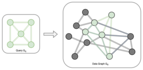
\includegraphics[width=\textwidth]{fig/LR/sgm-intro-double.png}
    \caption{Subgraph Enumeration Example}
    \label{fig:sgm-intro}
\end{figure}

Isomorphic graphs are of interest since they represent similarity between inherent topology of the graph.
% most graph properties do not depend on labels of vertices. \RN{<-unclear sentencee.}
% As graph data is mostly relational the similarity between inherent topology is captured by graph isomorphism. 
For graphs $G_1$ and $G_2$ graph isomorphism is a bijection between the vertex sets $\mathcal{V}(G_1)$ and $\mathcal{V}(G_2)$ $f: \mathcal{V}(G_1) \rightarrow \mathcal{V}(G_2) $ with the condition: \textit{any two vertices $u$ and $v$ of $G_1$ are adjacent in $G_1$ \textit{if and only if} $f(u)$ and $f(v)$ are adjacent in $G_2$}.
% Mathematically, for $G_1$ and $G_2$ to be isomorphic: $(u,v) \in \mathcal{E}(G_1) \leftrightarrow (f(u),f(v)) \in \mathcal{E}(G_2)$. Where \SV{Here,} $\mathcal{E}(.)$ represents the edge set of a graph. 
% \SV{Confusing. Maybe mention informally, define all the E, G terms first and then mathematically show what graph isomorphism is.} 
In this work we focus on undirected query graphs and data graphs.
Subgraph enumeration entails the subgraph isomorphism problem which is known to be NP-complete \cite{Book:Complexity_Theory}.

Subgraph Enumeration has wide range of applications.
For example, it can be used for plagiarism detection \cite{quasi-clique-plagiarism}, network motif counting \cite{motif-counting-application}, comparing similarity between large graphs \cite{large-graph-comparison-application}, designing bioinformatics networks \cite{bioinformatics-application}, chemical target structure synthesis \cite{chemical-target-application}, analyzing insights in recommendation networks \cite{recommendation-network-application}, etc.

% Demand for Data scalability
With the advent of \textit{Internet of Things} (IoT) and \textit{Information Technology} (IT), the sizes of graphs representing underlying data are substantially bigger and pose
%tough 
significant
challenges for data scalability.
Increasing interests in graph analytics and improvements to computational hardware over the last two decades, particularly in CPUs and GPUs have helped develop practical solutions to this computationally challenging problem.
Nevertheless, many existing solutions do not scale well with increasing template size due to issues like memory requirement, computational time, and load imbalance.

% My contribution

This work is focused on improving the existing state-of-the-art solution for subgraph enumeration: PARSEC, developed by Dodeja \etal \cite{PARSEC_VD}.
A series of enhancements were developed to improve its computational performance which are discussed in later sections. These enhancements include:
\begin{enumerate}
    \item Smart preprocessing techniques to detect intersection reuse and reduce computation.
          % \item Priority based sorting to reduce computation and eliminate overheads.
    \item Two-Phase strategy to improve symmetry breaking effectiveness.
    \item Hybrid parallelism for better load balance.
\end{enumerate}
%Rest of the chapters are 
The remainder of this thesis is organized as follows:
% Section summary
\begin{enumerate}[\indent {}]
    \item Chapter \ref{chap:Background} provides an overview of Graphics Processing Units and graph storage formats.
    \item Chapter \ref{chap:lit} is devotetd to a Literature Review that describes related work and defines mathematical notation used throughout this thesis.
    \item Chapter \ref{chap:basic-theory} illustrates basic techniques used in the subgraph enumeration algorithm with the help of a running example.
    \item Chapter \ref{chap:Improvements} describes the aforementioned enhancements in detail and analyzes their individual contribution to performance.
    \item Finally, Chapters \ref{chap:Results} and \ref{chap:conclusions} evaluate the combined improvement due to these individual enhancements and summarize the thesis with concluding remarks and scope for further work.
\end{enumerate}
	% for INTRODUCTION in "intro.tex"
\chapter{Background}\label{chap:Background}


\section{GPU Overview}\label{GPU-info}
% This section provides a brief overview of GPGPU and CUDA.
\subsection{History and Motivation}\label{sec:History}
In the world of computational hardware, microprocessors based on single processing cores (traditional CPUs) have driven rapid performance improvements in floating-point operations per second (FLOPS) for nearly 2 decades $(1985-2003)$.
These microprocessors were capable of performing in the range of Giga-FLOPS $(10^9)$ on desktops and Tera-FLOPS $(10^{12})$ on data centers \cite{GPU_book_wen-mei}.
This improvement drive flattened due to fundamental problems such as thermal stability, energy density, and quantum effects.
Since then, all microprocessors have adapted architecture with multiple processing cores and thread virtualization to keep up with the improvements expected by the market. Naturally, it needed significant change in software to keep up with the reported performance and increasing computational requirements \cite{Sutter-multi-core-programming}.

High-Definition Graphics demand from the gaming industry was one of the biggest drivers for such high-performance hardware. The performance demanded here is throughput oriented i.e., generating maximum frames per second while the computational requirement for each pixel is sufficiently low.
Some chip manufacturers like NVIDIA took a different approach of multi-thread hardware  to cater to these requirements \cite{GPUs_and_gaming}.
The hardware designed with this philosophy had threads capable of performing simple computational tasks with relatively lower clock speed to give an overall performance in Tera-FLOPS range. On top of that, the hardware gave more performance per watt which made it possible to add to a desktop machine \cite{ppw_gpu_vs_cpu}.
Modern GPUs have also proven to be fast and cost-effective for deep learning and image processing tasks contributing to many advances in fields like computer vision and artificial intelligence. A modern data center GPU, for example (NVIDIA A100), now has more than 100,000 concurrent threads. These threads execute in many simple pipelines to give around 10 times faster raw performance than state-of-the-art CPUs \cite{GPU_book_wen-mei}.
\begin{figure}
    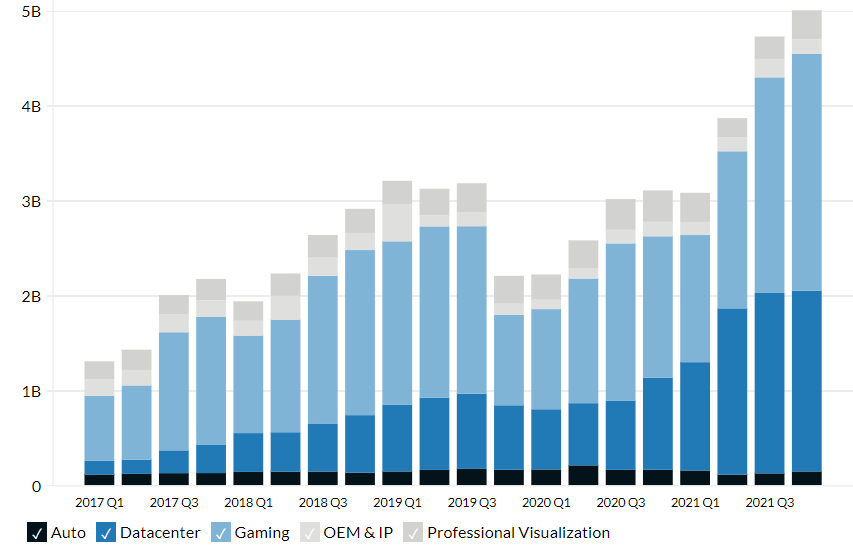
\includegraphics[width=\textwidth]{fig/Nvidia-revenue-by-end-market.png}
    \source{Business Quant \cite{business-quant}}
    \caption{Nvidia Revenue by End Market}
    \label{fig:Nvidia-revenue}
\end{figure}

Figure \ref{fig:Nvidia-revenue} shows that NVIDIA GPU data center market has improved significantly in recent years to become almost equivalent to the already huge gaming industry.
This has fueled the hardware and software development of current server-grade GPUs which has enabled huge computational potential for deep learning.
While HPC hardware improves at such rapid pace, software solutions for graph theory problems still need to move from the \textit{multi core} paradigm to \textit{multi thread}.

\subsection{Heterogeneous Programming Environment}
\begin{figure}[ht]
    \begin{minipage}{0.35\textwidth}
        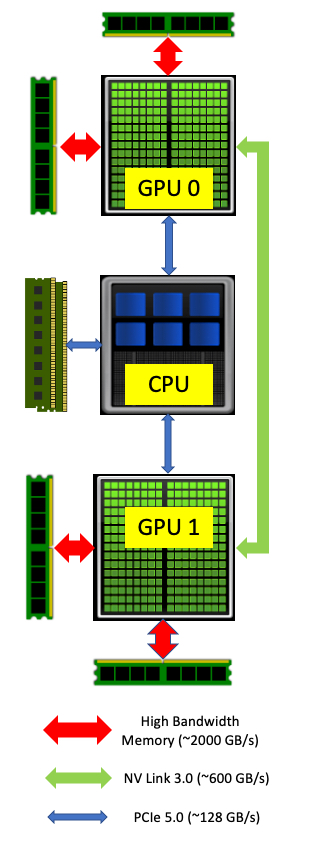
\includegraphics[width=\textwidth]{fig/cpu-gpu-arch.jpg}
    \end{minipage}
    \begin{minipage}{0.6\textwidth}
        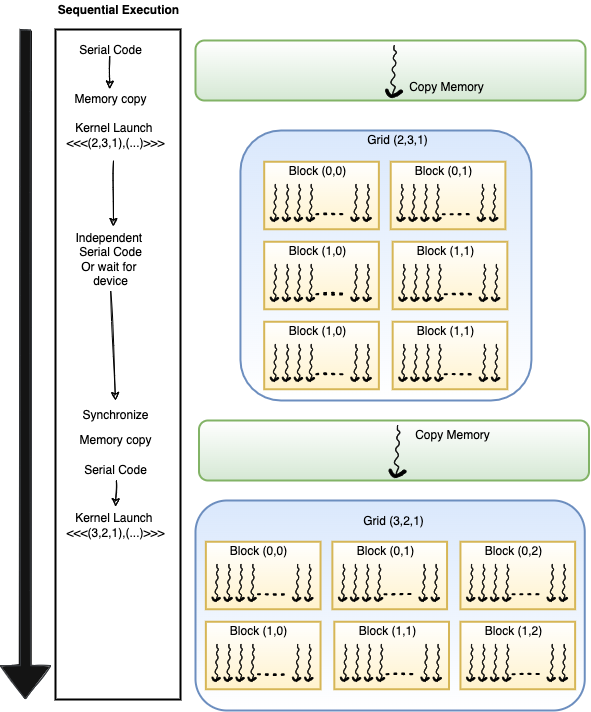
\includegraphics[width=\textwidth]{fig/heterogeneous-programming.png}
    \end{minipage}
    \caption{CUDA Heterogeneous Programming Model}
    \label{fig:Heterogenous-Programming}
\end{figure}
GPU is a throughput oriented computational hardware.
A single thread of a GPU is significantly slower than a CPU. Hence, working with it for inherently sequential tasks can incur huge latencies.
Since many basic programming tasks are inherently sequential and the whole operating system environment is developed for latency optimized processors (CPUs), GPUs work better off being used as a supplemental piece of hardware along with CPUs for computationally intensive tasks.
Hence, GPUs are mostly used in a Heterogeneous programming environment with CPU (host) executing the governing code while offloading computationally intensive tasks as kernels to GPUs (device).
Note that one host can be connected to multiple devices.
Since the memory of device and host are different, the input and output data need to be copied before and after kernel execution.
Figure \ref{fig:Heterogenous-Programming} shows the high level hardware and software architecture.
GPUs can communicate with CPU via PCIe (Peripheral Component Interconnect express) bus and with each other via NVLink \texttrademark.
The memory bandwidth of PCIe is the lowest and hence it is in best interests to avoid high data transfers between GPU and CPU.
Native memory of the GPU or the VRAM, is High Bandwidth Memory (HBM) with the latest generation having bandwidth of around 2000 GB/sec.
The Nvidia proprietary GPU Interconnect with 12 links per GPU can provide up to 600 GB/sec.
While the industry standard PCIe bus gen 5.0 with 32 links can provide up to 128 GB/sec of bandwidth.

\subsection{Thread Hierarchy}\label{sec:thread-hierarchy}
As discussed in Section \ref{sec:History} GPUs have \textit{multi thread} architecture with hundreds of thousands of threads. To have such massive hardware parallelism threads have to collaborate on usage of different resources for ex.\textit{cuda cores}.
%
Since all threads do not share these resources, it is important to understand thread Hierarchy in GPUs.

\begin{figure}[h]
    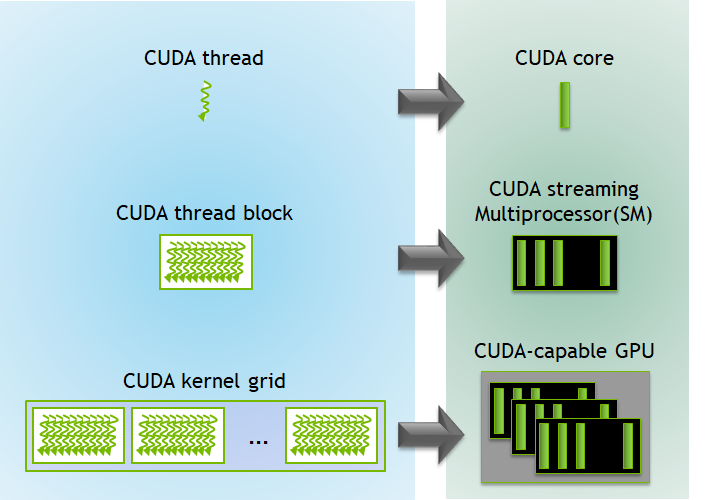
\includegraphics[width=\textwidth]{fig/thread-hierarchy.png}
    \source{Nvidia Developer Blog \cite{developer-blog}}
    \caption{Thread Hierarchy}
    \label{fig:Thread-Hierarchy}
\end{figure}

A thread is a single sequential flow of control within a program.
A block is a chunk of threads while a grid is a chunk of blocks.
Since threads are virtual they need to be optimally assigned hardware resources to perform tasks.
Figure \ref{fig:Thread-Hierarchy} shows how these virtual entities are mapped to the hardware. As discussed a thread utilizes a \textit{cuda core} for performing computation. A block of threads resides on a \textit{Streaming Multiprocessor} (SM), which is a hardware block that consists of computational resources like \textit{cuda cores, memory controllers, tensor cores}, etc. Thread block resides on an SM for the entirety of its execution. Hence, multiple threads in a block can utilize the same core. Multiple blocks can reside on an SM simultaneously within limits.
GPU has multiple SMs and hence many blocks can concurrently reside on the GPU during a context. If a grid requests more blocks than that can concurrently reside on the GPU, their execution is serialized.
Nvidia's latest server-grade GPU A100 has 108 SMs with a maximum of 32 blocks or 2048 threads residing per SM which means the maximum number of concurrent threads is  221,184. While on the hardware side, A100 has 6912 \textit{cuda cores}, i.e., 64 cores per SM.
% So, during execution, all 2048 threads in a block will compete for these 64 cores.

To add further, the thread instructions are processed in a Single Instruction Multi Data (SIMD) model. This SIMD chunk of threads is allocated resources at once, this chunk is called \textit{warp}. If threads within a warp demand different operations then all threads within that warp perform all operations with output of undesired threads being ignored. This causes a slowdown in execution and is referred as \textit{warp divergence}. Hence, algorithms and implementations need to be designed in such a way that \textit{warp divergence} is minimized. While the size of thread block and grid are configurable by the programmer, warp size is a fixed architectural parameter.

\begin{figure}[h]
    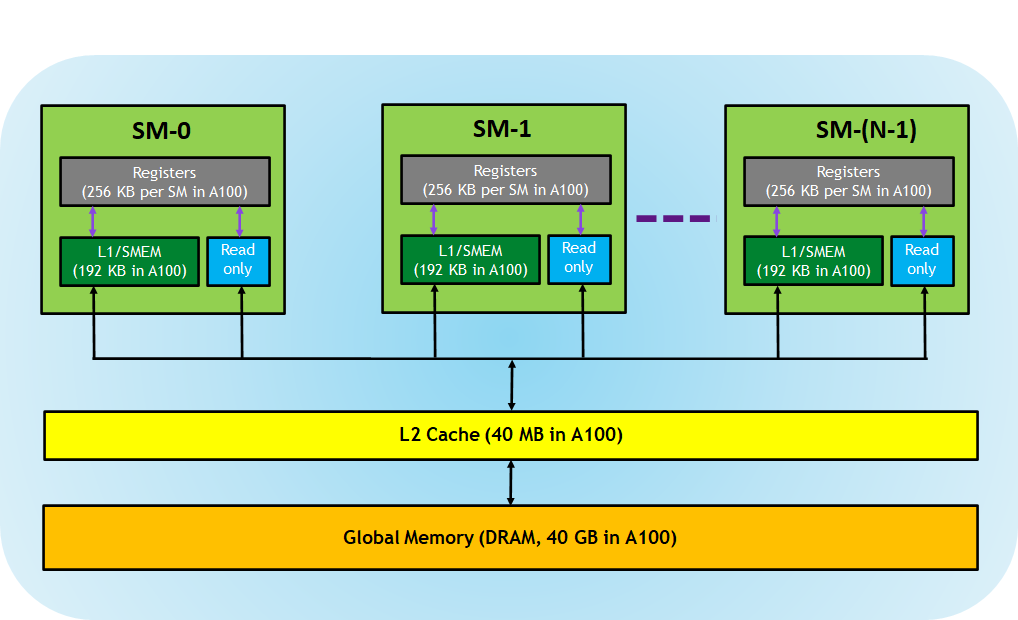
\includegraphics[width=\textwidth]{fig/memory-hierarchy.png}
    \source{Nvidia Developer Blog \cite{developer-blog}}
    \caption{GPU Memory Hierarchy}
    \label{fig:Memory-Hierarchy}
\end{figure}

\subsection{Memory Hierarchy}
GPU needs high performance memory system as it can be easily stressed due to the underlying massive parallelism.
If the available memory bandwidth is overwhelmed, threads need to wait for data to be able to perform computation even though some processing cores are free. This results in poor utilization and overall slower performance.
Even though GPU memory is significantly faster than conventional RAM, it can still limit application performance.
This problem is alleviated by building memory caches on the chip die itself, so accessing them is significantly faster (around 100 - 1000 times) but they have size restrictions.
Modern compilers identify repeated memory accesses and can aggressively cache to reduce memory stress.
The memory bandwidth problem is not significant for CPUs as they have huge cache banks per thread core. But for GPUs the cache per thread (L1 cache) is very restrictive.

GPU memory architects have tried to solve this problem by adding hierarchical memory banks. There are 3 types of memory banks on a GPU namely \textit{Global}, \textit{Shared} and \textit{Register} memory.
Figure \ref{fig:Memory-Hierarchy} shows the memory hierarchy, as name suggests global memory is accessible by all threads, it is equivalent to the Random Access Memory (RAM) on CPUs and is also sometimes referred as Video RAM (VRAM) or Device RAM (DRAM).
Shared memory is accessible by all threads in a thread block.
Register memory is private to each thread.
The size limitations on these memory banks are based on SM architecture and hardware.
Programmers are also equipped with read-only constant memory (not shown in the Figure \ref{fig:Memory-Hierarchy}) which is accessible by all threads.
Unknown to the programmer, compilers can also utilize these memory banks by caching in register and shared memory banks if repeated accesses to global memory are detected. It is referred as L1 cache. Equivalent to CPU cache there is also an L2 cache for use by the compiler only and accessible to all threads.

As discussed, memory utilization plays a significant role in code performance, a program whose execution time is restricted by memory is called memory bound. Memory bound programs do not scale well with increasing number of devices as distributing computation to other workers does no benefit and further increases latency due to communication.
Some common techniques to reduce memory pressure are designing algorithms capable of using shared and register memory, consecutive threads accessing nearby memory and reducing contention for atomic operations on global memory.



\subsection{Block Scheduling}\label{sec:block-scheduling}
As discussed in Section \ref{sec:thread-hierarchy} many blocks can concurrently reside on a GPU.

Generally kernels are launched with grid sizes much higher than that can concurrently reside on a GPU, so the block execution needs to be serialized once maximum number of blocks that can occupy the GPU are scheduled, the blocks waiting after initial allocation are allocated resources as they become available (i.e. a scheduled block terminates).
This is done as blocks are non-preemptive. That is, ones allocated resources the block is never unallocated till its completion.
This scheduling provides scope clever memory utilization as memory need not be allocated for whole grid but only the blocks that can run concurrently. This concept of memory management is called persistent memory, using it can help reduce memory requirements.

Since blocks are preemptive, it is important to design the parallelism in such a way that all blocks have nearly similar amount of work.
If not, blocks having higher amount of work should be scheduled earlier to reduce make span.
In order to have better control over work allocation to a block, programmers often launch kernels with grid size equivalent to that can concurrently reside.
These blocks then can choose from a common list of tasks in global memory, this approach is known as work stealing.
Work stealing makes sure that work is allocated to a worker as soon as it is free.



\section{Graph Storage}\label{storage-format}
Graphs can be stored in various formats, a suitable format is selected based on hardware and software constraints/requirements.
\textit{Adjacency Matrix} and \textit{Adjacency list} representations are amongst the most elementary storage formats.
As the name suggests, \textit{adjacency list} format is stored as an array of lists where $i^{th}$ element of the array stores a list of neighbors of vertex \textit{i}.
\textit{Adjacency Matrix} format stores the relational information in a boolean matrix format.
Let the underlying graph be $G=(V,E)$ and its adjacency matrix representation be A.
Then $A = |V|\times|V|$ is defined as:
$$
    A_{i,j}=\begin{cases}
        1 & (i,j) \in E      \\
        0 & \text{Otherwise}
    \end{cases}
$$

For most real world graphs, the underlying adjacency matrix is sparse. Hence, it is effective to be stored in sparse matrix formats.
The computing community uses various sparse matrix formats such as \textit{ELL-Pack} (ELL), \textit{COOrdinate} (COO), \textit{Compressed Sparse Column} (CSC), \textit{Compressed Sparse Row} (CSR), \textit{Blocked Compressed Sparse Row} (BSR), etc.


\begin{figure}[h]
    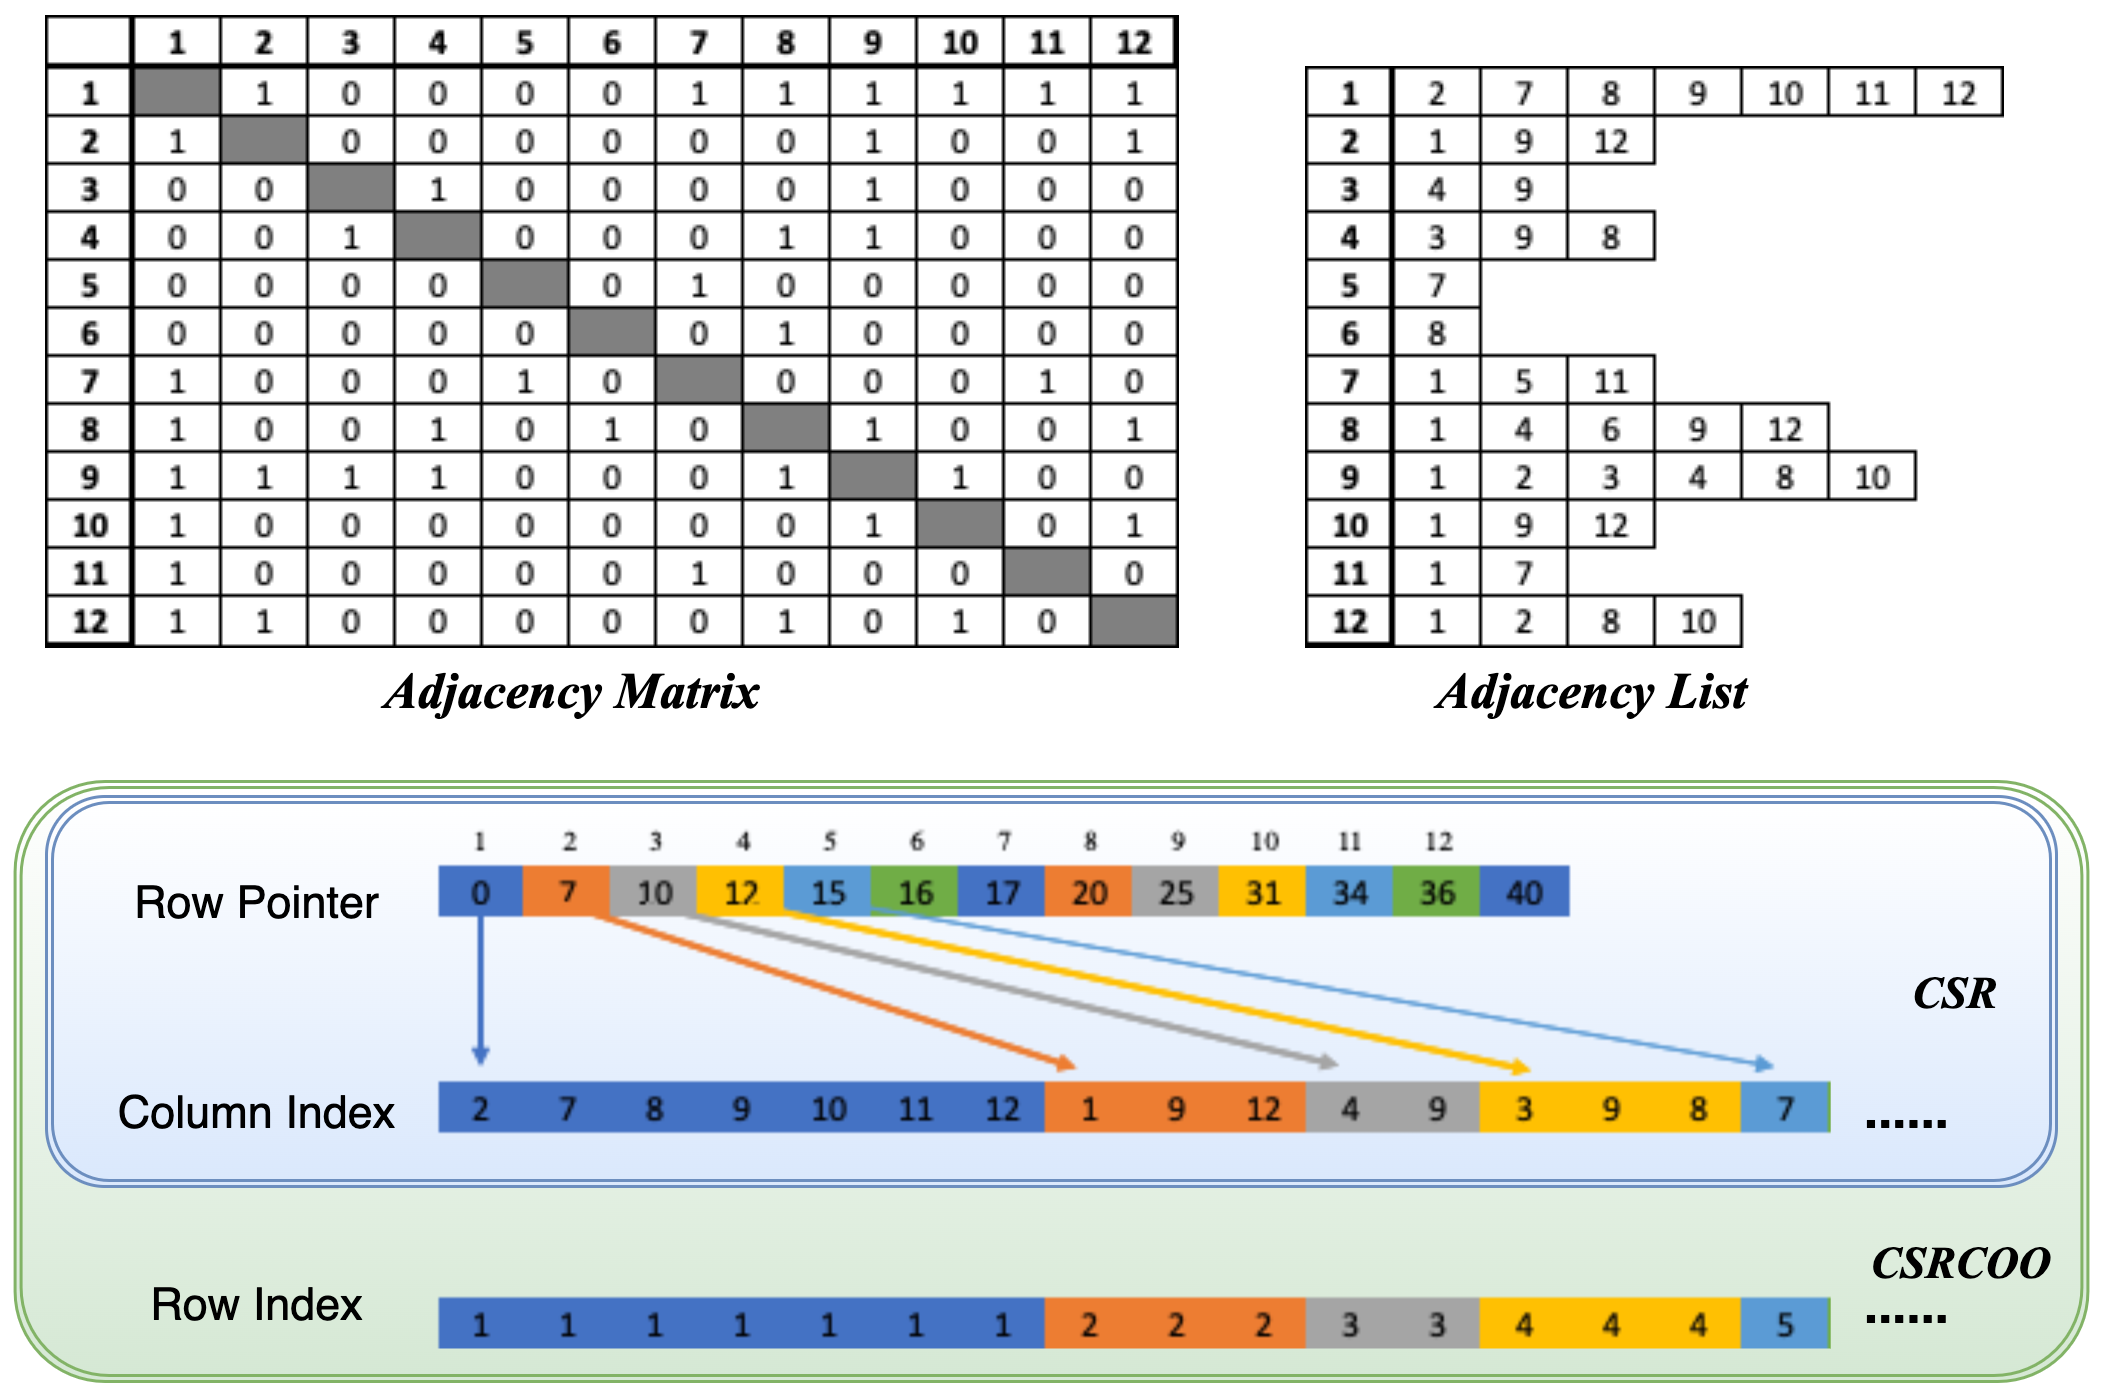
\includegraphics[width=0.9\textwidth]{fig/graph-storage.png}
    \caption{Graph Storage Formats for graph in Fig.\ \ref{fig:sgm-intro}}
    \label{fig:graph-storage}
\end{figure}

We use a combination of CSR and COO formats in our implementation, it is referred as the CSRCOO (Column Sparse Row with COOrdinate) format.
The CSRCOO format uses 3 arrays for storing information of the underlying graph.
These arrays are \textit{Row Pointer} (length: $|V|+1$), \textit{Row Index} (length: $|E|$) and \textit{Column Index:} (length: $|E|$).
% Here the first 3 arrays are same as the standard CSR and COO arrays, the $4^{th}$ array stores the column indices in a segment wise sorted fashion based on a given rule.
% We use Degree and Degeneracy as 2 rules in this work.
We maintain the \textit{Row Index} and \textit{Column Index} arrays sorted by their labels to enable binary search.
Figure \ref{fig:graph-storage} shows comparison between different graph storage formats.
% \samiran{Anything else that should be added?}
\chapter{Literature Review}\label{chap:lit}

This chapter describes relevant work in the area of subgraph enumeration in sequential (CPU) and parallel computing (multi-core/GPU) communities.
First, some definitions and notation are established to develop formal understanding.

\section{Notation and Definitions}
A graph is a pair of sets $G=(V,E)$, where $V$ is a set of elements called vertices and $E$ is a set of vertex pairs whose elements are called edges.
An edge is represented by the elements in the vertex pair $(u,v)$.
$u, v$ are called the endpoints of the edge.
Edges of the graph can be directed or undirected.
Undirected edges imply \{$(u,v)\in E \Leftrightarrow (v,u) \in E \quad \forall ~ u, v \in V$\}.
An edge $e = (x,y)$ is incident to a vertex $v$ if $x=v$ or $y=v$.
In this work, all graphs have undirected edges unless specifically mentioned.
Graphs with directed Edge set are called directed graphs.
$\mathcal{V}(G)$  and $\mathcal{E}(G)$ denote the vertex and edge set of graph $G$, respectively.

Neighbor set of a vertex $v$, denoted by $\mathcal{N}(v)$, is a set of all vertices $u$ such that $\{u \in \mathcal{N}(v) \Leftrightarrow (u,v) \in E$\}.
In case of a directed graph the neighbors are further categorized as \textit{forward/outgoing} neighbors and \textit{backward/incoming} neighbors based on the direction of the incident edge.
Degree of a vertex $v$, denoted by $d(v)$ or $degree(v)$ is the cardinality of its neighbor set, i.e., $d(v)=|\mathcal{N}(v)|$.
Maximum degree of a graph is the maximum of all degrees from its vertex set.
Oriented graph is a transformation of an undirected graph $G$ to a directed graph $\tilde{G}$ such that: $$\{\forall~ (u,v) ~\& ~ (v,u) \in \mathcal{E}(G), \text{ either } (u,v) \text{ or } (v,u) \in \mathcal{E}(\tilde{G})\}$$


A subgraph $g$ of a graph $G$, denoted by $g \subseteq G$ is a graph $g=(V_g, E_g)$ such that $V_g \subseteq V$ and $E_g \subseteq E$ where, $\forall~ (u_g, v_g) \in E_g \Rightarrow u_g, v_g \in V_g$.
Induced subgraph by a vertex $v'$ in graph $G$, denoted by $G(v')$ is a subgraph $g=(V', E')$ of $G$ such that $V'=\mathcal{N}(v')\cup \{v'\}$ and $\{(x,y) \in E'\Leftrightarrow {x,y} \in V'\}$.

For the rest of this thesis, the data graph is denoted by $G_d$ and the query graph is denoted by $G_q$. $V_d =  \mathcal{V}(G_d), V_q = \mathcal{V}(G_q)$.
As introduced previously, the subgraph enumeration problem is to find all instances of $G_q$ that are isomorphic to $G_d$.
Isomorphism is a bijection $f$ between vertex set of two graphs, here $G_q$ and $g \subseteq G_d$, such that $ (u,v) \in \mathcal{E}(G_q) \Leftrightarrow (f(u), f(v)) \in \mathcal{E}(g)$.

As we will see in Section \ref{sec:LIT-r}, the traversal based algorithms for subgraph matching consist of routines for converting a given query graph to a directed graph and matching each vertex in the query graph to suitable vertices in the data graph. Whenever there is more than one match, each has to be considered independently.
This creates branches and constructs a tree which is called the \textit{search tree}.
The order in which the data graph vertices are matched with the query graph is called the \textit{match order}.
Formally, given $G_q$, the match order $\pi$ is the permutation of vertices $V_q$ which reflects the order in which they will be matched.

\section{Related Work} \label{sec:LIT-r}
The underlying routine of subgraph enumeration is graph isomorphism.
The first algorithm for detecting graph isomorphism was given by Ullman \cite{ullman_sgm}. In this algorithm, an isomorphic subgraph was found using a brute force search tree traversal with elimination of successor nodes.
The traversal used was DFS with each instance being represented as a binary table of $|V_q|\times |V_d|$ entries.
For finding all instances, a DFS is recursively performed on all possible candidates with some of them pruned in advance.
These search tree based algorithms are sometimes also referred to as \textit{state space search} algorithms.

Some other promising techniques which perform traversal to find query instances are exploration \cite{expl-based1}, \cite{expl-based2}, \cite{expl-based3}, \cite{expl-based4} and constraint programming \cite{cp-based-sgm1}, \cite{cp-based-sgm2} based.
Approaches which do not perform traversal are based on converting query instances to a multi-way join framework where the edges represent relations in $G_q$ and evaluate the multi-way join to find all results \cite{mapreduce}, \cite{mapreduce-dist}.
However, these techniques perform better for labeled subgraph enumeration \cite{sgm-techniques} and hence will be ignored in this review.

The algorithm of Ullman \cite{ullman_sgm} formed the basis for various subsequent traversal based algorithms. Improvements came from different pruning heuristics and better match ordering. These algorithms are explained in Section \ref{sec:lit-seq}.
Most sequential algorithms perform state space search process at each root node.
With advancements in multi-core processors and cloud computing servers, multiple scalable algorithms were developed, which are mentioned in Section \ref{sec:lit-par}.
Most recently, the focus has shifted to GPUs because of increasing memory capacity and their advent in compute servers; these contributions are mentioned in Section \ref{sec:lit-gpu}.

\subsection{Sequential Algorithms} \label{sec:lit-seq}
Vento and Fogia (VF) \cite{VF} reduced the memory requirements of \cite{ullman_sgm} by using a State Space Representation (SSR) and developed a deterministic matching method for simultaneously verifying isomorphism.
VF2 \cite{VF2} introduced five feasibility rules for early pruning of the search tree to shrink the search space.
VF3 \cite{VF3} developed multiple additional heuristics for early pruning and further reduced the search space. These heuristics were developed with the help of extensive computational experimentation.
Grochow \etal \cite{symbreak} assigned partial ordering to vertices matched with symmetrical query vertex to reduce redundant work.
$\text{Turbo}_{\text{iso}}$ \cite{Turbo-iso} improved match ordering by dynamically computing a match order for each candidate that made the search tree leaner and provided performance improvement.
$\text{Boost}_{\text{iso}}$ \cite{Boost-iso} in a novel contribution utilized vertex relationships to efficiently arrange candidate vertices to reuse adjacency list intersections.

These sequential algorithms offer great insights into the search tree exploration phase.
Since the problem has so much independent work, a sequential processor tends to be slower due to repetition of tasks.
Hence, sequential implementations are only practical for data graphs with up to 100,000 vertices.
Many techniques used by parallel algorithms for shrinking search space arise from sequential algorithms.

\subsection{Multi-core Algorithms} \label{sec:lit-par}
Parallel Subgraph Listing \cite{psgl} was the first truly parallel search space traversal based algorithm on multi core hardware. It introduced a subgraph listing framework that statically divided work across multiple threads.
Various load balancing strategies were developed to improve its performance. It was also proved that the problem of partial subgraph distribution for workload balance is strongly NP-Hard.
CECI \cite{CECI} proposed a novel framework for Subgraph Listing based on Compact Embedding Cluster Index, which divides the data graph into multiple embedding clusters for parallel processing.
Despite orders of speedups and scalability, the technique uses BFS and needs huge amount of memory for storing intermediate results.
LIGHT \cite{LIGHT} eliminated the memory requirements of previous BFS parallel algorithms by developing a multi-threaded DFS framework.
Dryadic \cite{Dryadic} is the current state-of-the-art CPU subgraph enumerator that uses a robust computation tree structure which optimizes queries by mapping them to different backend hardware to perform custom compiled graph pattern matching.

To summarize, multi-core algorithms easily outperform  sequential algorithms but are limited by the parallelism offered by CPUs.
Memory bandwidth across different nodes makes it further difficult to scale.
BFS-based strategies are prevalent in the parallel computing community, which impose huge hardware requirements due to significant memory usage.

\subsection{GPU algorithms} \label{sec:lit-gpu}
Due to the advancements in graph algorithms on GPUs like max-flow, shortest paths, and spanning trees, many state space traversal based subgraph enumeration algorithms were developed.
To the best of our knowledge, GPSM \cite{GPSM} is the first subgraph enumeration implementation on GPU.
It used advances in BFS on GPUs to implement the basic search tree traversal procedure.
GPSM outperformed the most advanced multi-core algorithm of its time by an order of magnitude in speedup.
RPS \cite{RPS-paper} focused on reducing the number of set intersection operations, since this is the most expensive computational step, by deploying a reuse framework in BFS traversal.
PBE \cite{PBE-paper} developed a scalable framework by using graph partitioning strategies to enable multiple GPUs to work on each partition.

Since all BFS-based approaches explode in memory requirements, PARSEC \cite{PARSEC_VD} developed the first DFS-based subgraph enumeration on GPUs.
It reduced the search space by limiting compatibility to queries with at least one fully connected node (\textit{central node}).

PARSEC \cite{PARSEC_VD} is selected as a baseline for our computational experiments. It clearly showed that DFS-based techniques are superior to the traditional BFS approaches on GPUs.
However, it performs redundant work due to the unavailability of intermediate candidates and multiple processing units working on the same subtree.
The parallelism schemes used by PARSEC also have severe load imbalance that hampers its performance.
We utilize the DFS framework developed by PARSEC along with different techniques from the traditional sequential and modern parallel algorithms to further improve its performance.
\chapter{Basic Techniques}\label{chap:basic-theory}

The Subgraph Enumeration algorithm can be decomposed into three major steps: (1) Query Graph Preprocessing, (2) Data Graph Preprocessing, and (3) Search Tree Traversal. This chapter covers each step in detail with a running example.

\begin{figure}
    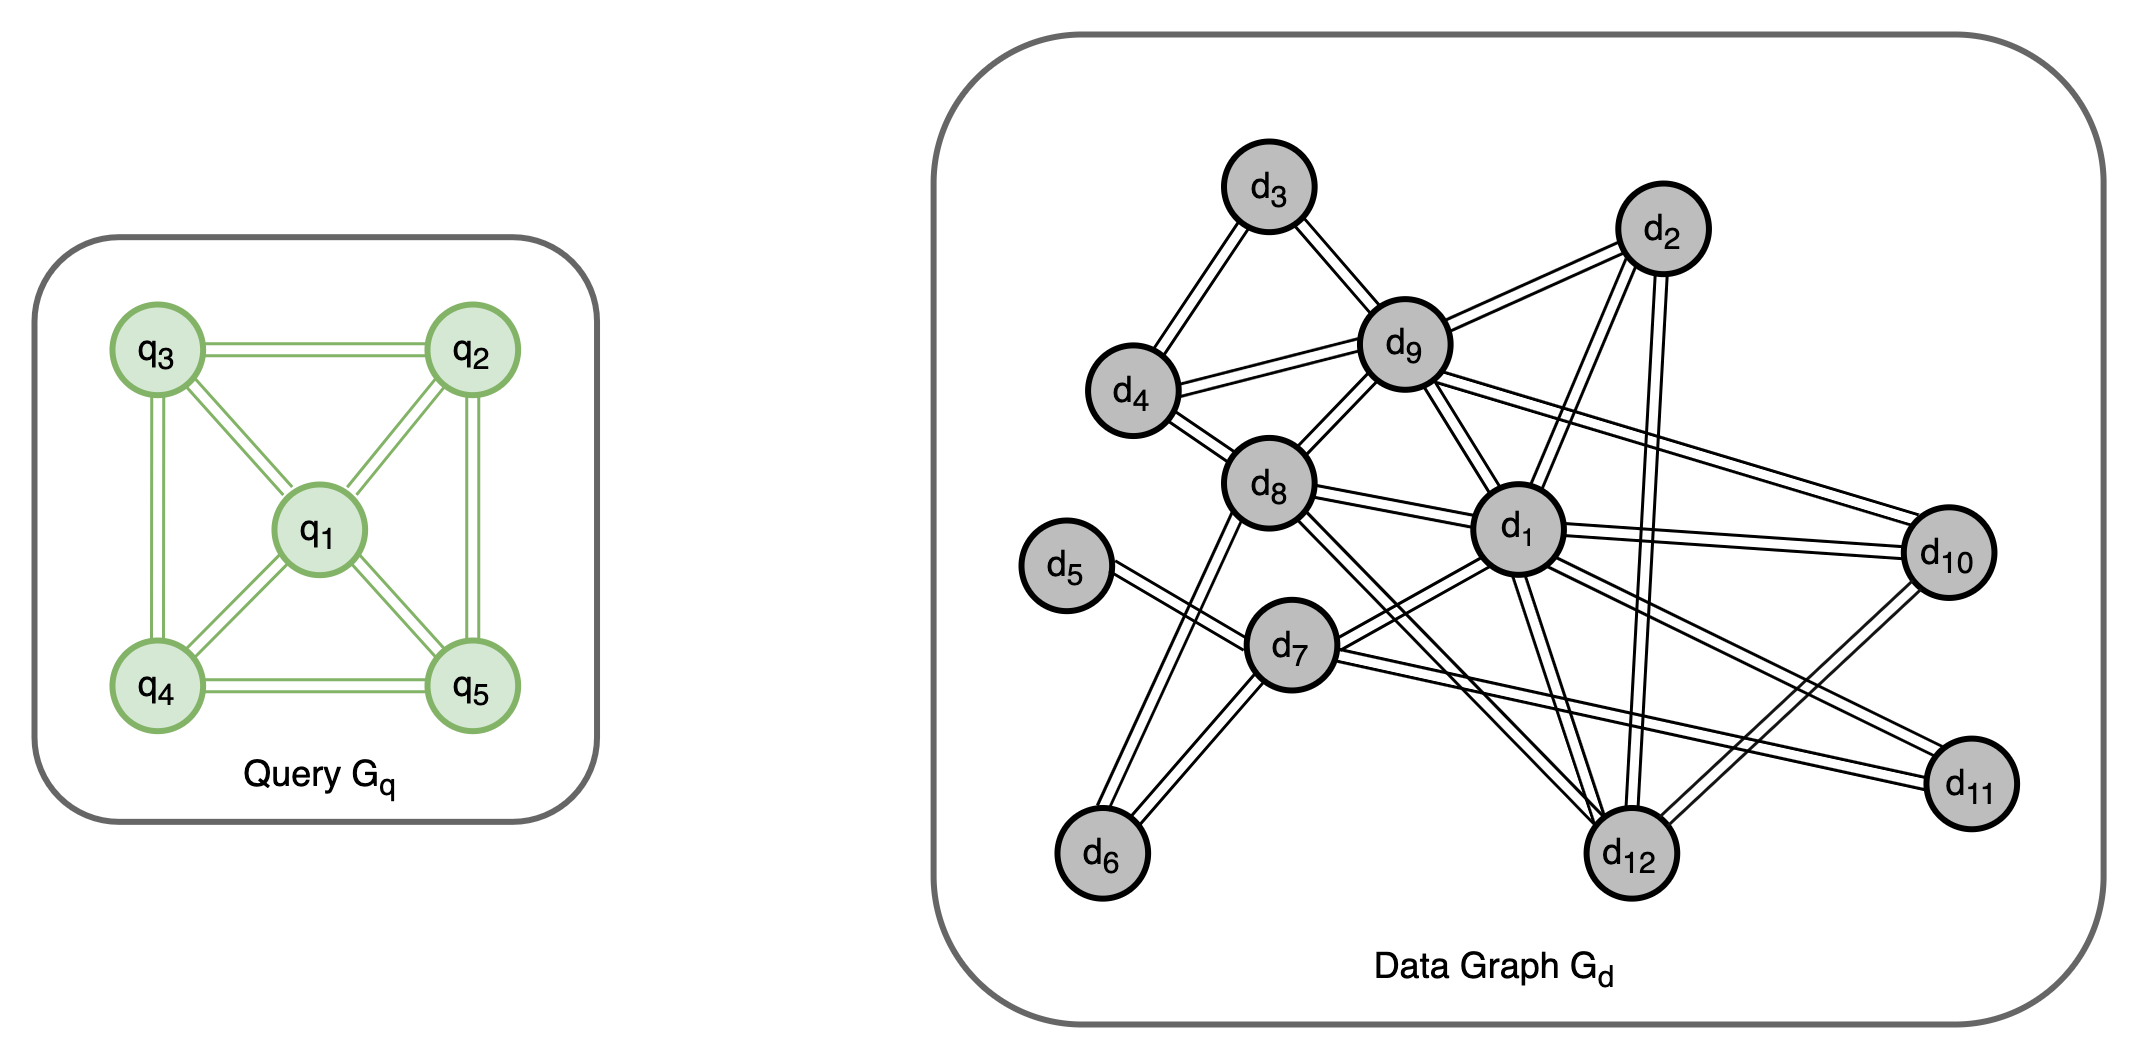
\includegraphics[width=\textwidth]{fig/LR/sgm-example1.png}
    \caption{Example}
    \label{fig:sgm-example}
\end{figure}
\section{Query Graph Preprocessing}\label{query-preprocessing}
This section explains all processing done on the query graph to enable it for search tree traversal
% \RN{the assumption is that somewhere previously you have explained that SE is performed using tree traversal; otherwise this appears to come out of nowhere}

There are three main tasks performed on the input query: (1) Query sequencing, (2) Symmetry Detection, and (3) Reuse Analysis. Since the query graphs are very small (less than 10 nodes, in general) and all preprocessing tasks are polynomial time complexity, this preprocessing workload is handled by the CPU.
Query preprocessing is important to shrink search tree exploration, the amount of work done at each node, and redundancy elimination.
% \RN{too many details that the readethewould not know about...}
% \samiran{Will try to introduce these in the literature review}.

\subsection{Query Sequencing}
The query graph input to the application is undirected. The first task is to convert this undirected graph to a directed acyclic graph (DAG). The ordering of the DAG governs the order in which these vertices are matched to the data graph.
The query nodes are ordered based on their likelihood of matching with the data graph. Naturally, query nodes with lesser likelihood are prioritized over others.

The query sequencing algorithm used by VF3 \cite{VF3} is utilized for this task. This algorithm uses multiple criteria to estimate the likelihood of matching and sequences the nodes in decreasing order of that likelihood. Interested readers are encouraged to read about these criteria in \cite{VF3}. Pseudocode for the algorithm used is listed in Algorithm \ref{algo:query-seq}.

\begin{algorithm}[h]
    \caption{Query Sequencing}
    \label{algo:query-seq}

    \SetKwData{dm}{$d_M$}
    \SetKwData{deg}{Degree}
    \SetKwData{lh}{likelihood}
    \SetKwData{i}{i}
    \SetKwData{j}{j}
    \SetKwData{idx}{idx}
    \SetKwData{seq}{$S_q$}

    \SetKwFunction{argmax}{argmax}

    \KwIn{Template Graph, $G_q$}
    \KwOut{Node Query Sequence, $S_q$}
    $\dm[N_q] \leftarrow 0$\;
    $S_q \leftarrow \phi$\;
    \For{$\i \leftarrow$ 0 \KwTo $N_q$}{
        \tcp{calculate likelihood for remaining nodes}
        \For{$\j \leftarrow 0$ \KwTo $N_q$}{
            \If{\j not in \seq } {
                $\lh[\j] \leftarrow \dm[\j] \cdot N_q + \deg[\j]$\;
            }
        }
        \tcp{Find node with maximum likelihood and it to \seq}
        \idx $\leftarrow$ \argmax{\lh}\;
        append \idx to \seq\;

        \tcp{Update \dm}
        \ForEach{neighbor \j of node \idx}{$\dm[\j] \leftarrow \dm[\j] + 1$\;}
    }
\end{algorithm}

The order generated after performing query sequencing on the example query graph is shown in Figure \ref{fig:query-sequencing}.

\begin{figure}
    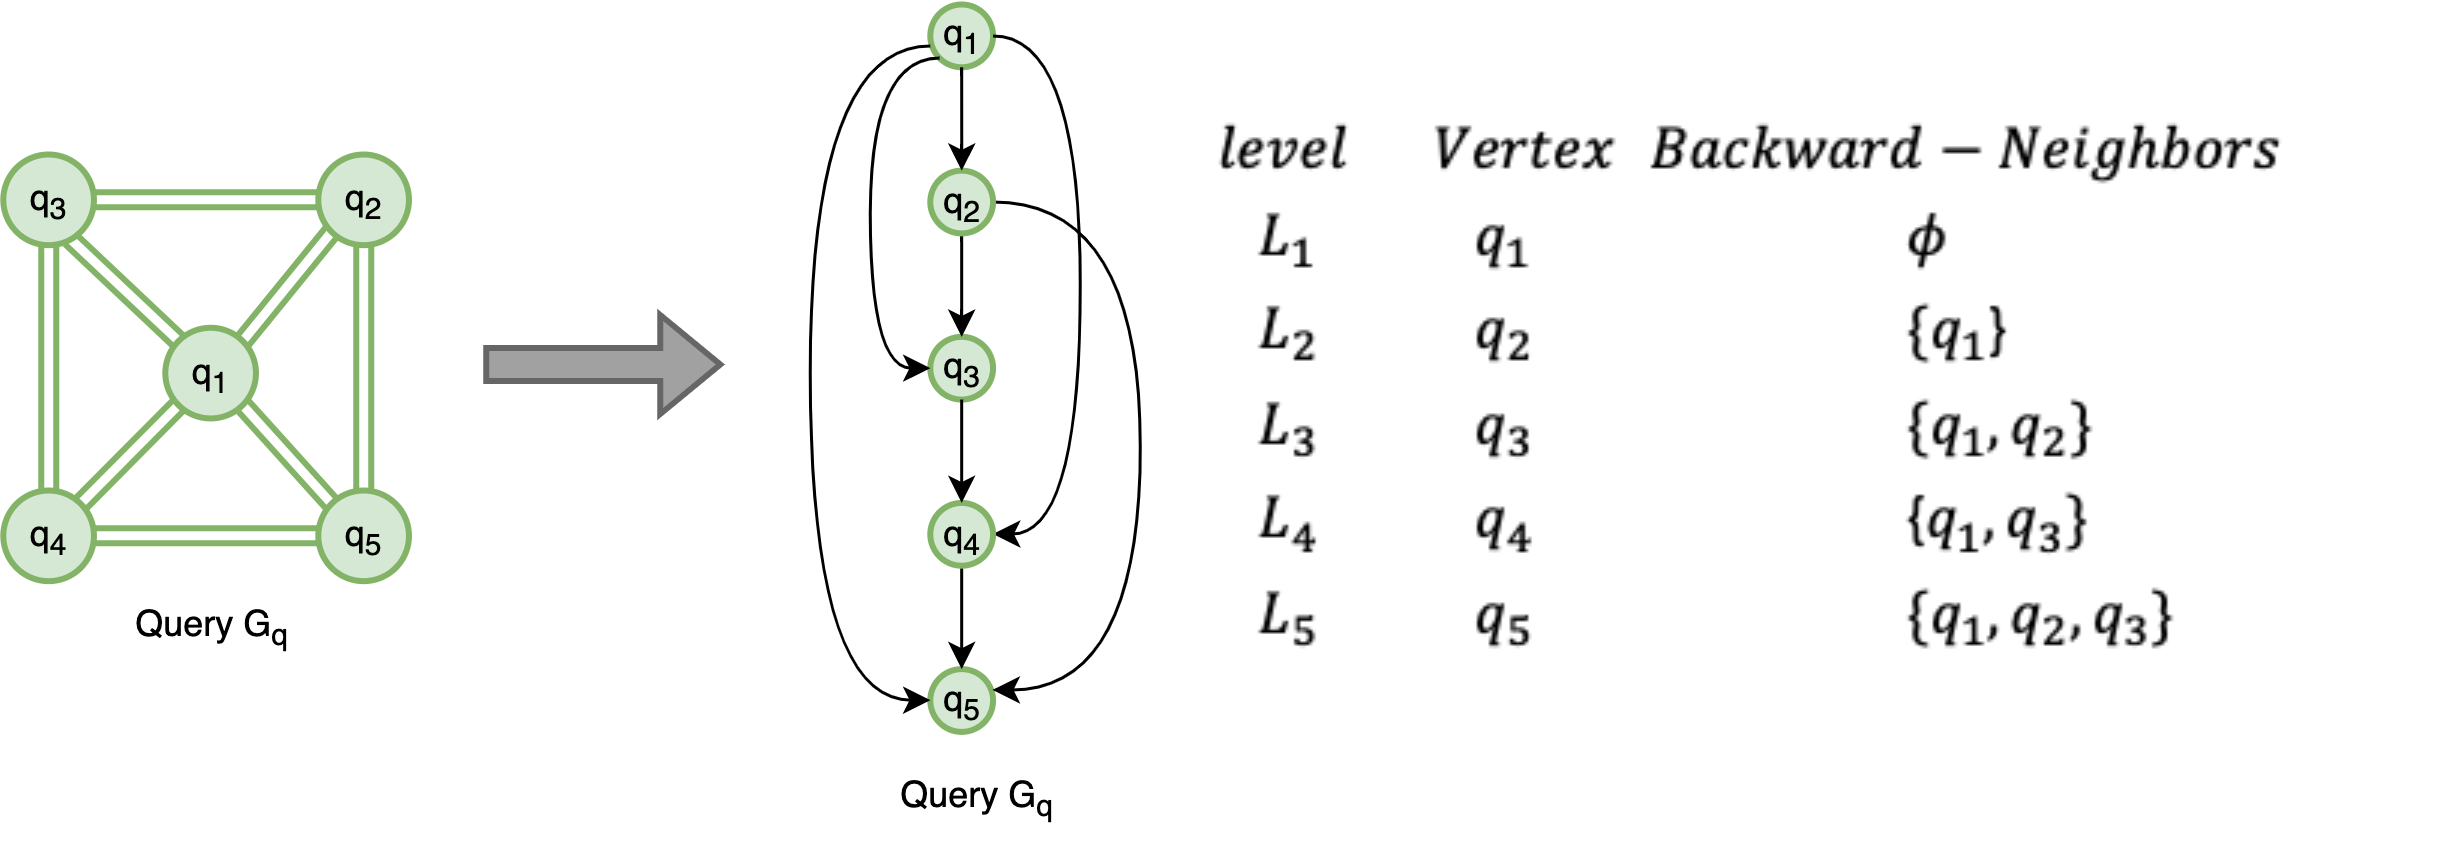
\includegraphics[width=\textwidth]{fig/LR/query-sequencing.png}
    \caption{Query Sequencing output of $G_q$ using \textit{VF3}}
    \label{fig:query-sequencing}
\end{figure}

\subsection{Symmetry Detection and Breaking}\label{sec:sym-detection}
Symmetry is the existence of automorphism in a graph. Automorphism, as the name suggests, is a graph that is isomorphic to itself.
An automorphism of a graph is a permutation of vertices that maintains edges and non-edges.
% Formally, an automorphism of a graph $G=(V,E)$ is  permutation $\sigma$ of the vertex set $V$ such that the pair of vertices $(u,v)$ form an edge if and only if $(\sigma(u), \sigma(v))$ also forms an edge.
The set of automorphic permutations of the vertex set is called the ``automorphism group".
Figure \ref{fig:automorphism} shows the automorphism group of the query graph $G_q$.
\textit{Orbit} is an equivalence class of vertices in the automorphism group.
\begin{figure}
    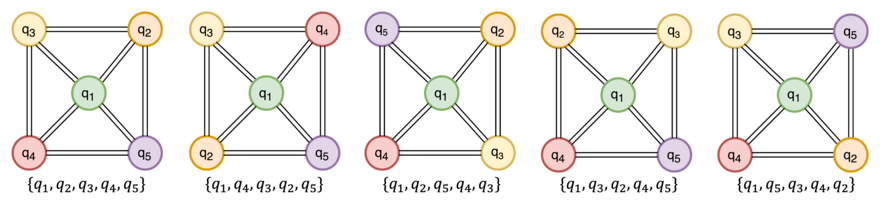
\includegraphics[width=\textwidth]{fig/LR/automorphism.png}
    \caption{Automorphism group of $G_q$}
    \label{fig:automorphism}
\end{figure}

The presence of symmetry essentially causes the same subgraph of the data graph to be counted multiple times and hence resulting in extra work and redundant counts.
The easiest technique that can be employed to avoid this is called symmetry breaking. This makes sure that the ties are resolved at the moment they are generated, hence avoiding redundant work.
An easy way to break symmetry is by having an order between the matches of data graph between the symmetric levels, this was first
% \RN{sure? how about previously} %
used by \cite{symbreak}. Algorithm \ref{algo:symbrk} lists the pseudocode for detecting symmetry and generating ordering for symmetry based pruning. Note, the \textit{GetAutomorphismGroup} and \textit{GetOrbits} routines used here are provided by NAUTY \cite{nauty}.
% \RN{Where are the functions GetXYZ/}

\begin{algorithm}
    \caption{Symmetry breaking}
    \label{algo:symbrk}
    \SetKwFunction{gag}{GetAutomorphismGroup}
    \SetKwFunction{gorb}{GetOrbits}
    \KwIn{Template Graph, $G_q$}
    \KwOut{Set of partial node orderings, $\mathcal{P}_q$}
    $\mathcal{A} \leftarrow$ \gag{$G_q$}\;
    \While{$\mathcal{A} \neq \mathbb{I}$}{
        $\mathcal{O}_\mathcal{A} \leftarrow$ \gorb{$\mathcal{A}$}\;
        Pick largest orbit $\{v_1, v_2, \dots, v_k\}$ from $\mathcal{O}_\mathcal{A}$\;
        Add $v_1 < v_2, v_1 < v_3, \dots, v_1 < v_k$ to $\mathcal{P}_q$\;
        $\mathcal{A} \leftarrow \{\alpha | \alpha\in\mathcal{A}, \alpha(v_1) = v_1 \}$\;
    }
\end{algorithm}


For example, to avoid redundancy due to automorphism $\{q_1, q_4, q_3, q_2, q_5\}$ of $G_q$, it can be made sure that the data graph vertices matched at level 2 have labels less than the vertices matched at level 4. This is an example of \textit{lexicographic symmetry} breaking.
Another symmetry breaking order can be the degree of data graph nodes themselves.
A key observation is that the symmetry breaking criteria can be different for different levels but not always different for different subtrees.
This will be formally established and utilized in Section \ref{sec:hy-symbreak}.

% \iffalse
%     \subsection{Reuse Detection}\label{sec:reuse-detection}
%     Set intersection operation for generating candidates at the next level is the most time-consuming operation in subgraph enumeration, this is a well-known fact in the literature and also re-verified in section \samiran{cite stacked bar graph figure}.
%     While traversing the search tree each node needs a set intersection operation on adjacency lists of backward neighbors (vertices matched with levels connected at the next level).
%     The number of backward neighbors at each level increases with increasing template size. This results in even more adjacency list intersections at each level.
%     RPS \cite{RPS-paper} reduces these operations by generating an intersection reuse plan, this plan smartly finds the intersections that will be required by more than one node and stores them when first calculated. There is a lot of intersection reuse possible with RPS as they employ a BFS strategy.
%     Similar reuse is not possible in DFS traversal since the past information is lost while backtracking.
%     However, Some levels of the sequenced query graphs have similar backward neighbor lists. For such queries' the majority of intersections can be reused by simply storing the intermediate intersection results. This technique is discussed in detail in Section \samiran{cite improvements section}.
%     To do this efficiently, the problem of finding level mappings with the most similar adjacency lists is posed as a linear programming optimization problem.

%     Let, the sequenced query graph be $G_q=(V_q, E_q)$ with $|V_q|=k$ and the vertex sequence $S_q$.
%     $\mathcal{N}(.)$ be the function for getting the backward neighbor list of a vertex.
%     For each pair of vertices at level $i$ and $j$ let $W_{ij}$ be a measure of the commonality between their backward neighbors' lists. Let $X_{i,j}$ be the decision variable which tells if vertex $i$ should reuse intersections from vertex $j$.

%     With these definitions the optimization problem can be modelled as:
%     \begin{align}
%         \max \sum_{i=j+1}^{k}\sum_{j=1}^{k} W_{ij} X_{ij} \\
%         \text{s.t.}
%         \sum_{j=1}^k X_{ij} \leq 1. \quad \forall i \in \{1, \dots, k\}
%     \end{align}
%     Where, $$
%         W_{ij} = \begin{cases}
%             |\mathcal{N}(S_q[i]) \cap \mathcal{N}(S_q[j])| \qquad \text{if} \quad i>j, \mathcal{N}(S_q[i]) \supseteq \mathcal{N}(S_q[j]) \\
%             0   \qquad \text{Otherwise}
%         \end{cases}
%     $$
%     This problem is a linear semi-assignment problem (LSAP) with the optimal solution being the greedy solution itself.
%     This is easy to establish as any other solution can be improved by switching to the greedy solution.
%     The solution to this problem is:
%     $$
%         X_{ij}=\begin{cases}
%             1   \qquad \text{if } j=\argmax_j(w_{ij}>0); \\
%             0   \qquad \text{Otherwise}
%         \end{cases}
%     $$

%     Reuse detection involves a find minimum operation for each level in $G_q$ hence it is polynomial time and can be performed on CPU for small-sized query graphs. Once, this is performed, it gives the levels that are \textit{reusable}. The intersection results for these levels are to be stored, this is discussed in detail in Section \ref{sec:reuse-impl}.

%     \newpage
% \fi

\section{Data Graph Preprocessing}\label{graph-preprocessing}

Data graph preprocessing involves operations on the data graph to shrink the search tree during traversal.
With GPU implementations, preprocessing also helps to improve coalesced memory accesses and saves on GPU memory.


\subsection{Peeling}\label{peeling}
Subgraph Enumeration produces isomorphic matches of query graph in the data graph.
Naturally, each match needs to have degree greater than the degree of the corresponding query node it is matched with.
This implies that: \textit{Vertices in data graph with degree less than minimum query degree will never form any matches.}
Using this simple observation, all the vertices with degree lesser than the minimum query degree are deleted from the data graph. This can be done iteratively as the lemma holds for the resulting data graph as well. This process is commonly called \textit{Peeling}.
Empirical experiments performed by \cite{PARSEC_VD} show that, for best results, \textit{Peeling} should be performed till at most $5\%$ of nodes are deleted.
Algorithm \ref{algo:peel} shows the pseudocode for the peeling routine.
Note the filtering of vertices is done on GPU using the CUB library \cite{cub}.
\begin{algorithm}[h]
    \caption{Peeling data graph}
    \label{algo:peel}

    \SetKwData{nfs}{PrunedVertices}
    \SetKwData{efs}{PrunedEdges}
    \SetKwFunction{d}{Degree}

    \KwIn{ Minimum query graph degree, $d_{q,min}$, $G_d = (V_d, E_d)$:}
    \Repeat{$|\nfs| < 0.05 \times |V_d|$}{
        \nfs $\leftarrow \{u | u \in V_d, \d{u} < d_{q,min}\}$\;
        \If{$|\nfs| = 0$}{\text{Break;}}
        $\efs \leftarrow \{(u, v) | u \textbf{ or } \in \nfs  $\;
        $V_d \leftarrow V_d \setminus \nfs$\;
        $E_d \leftarrow E_d \setminus \efs$\;
    }
\end{algorithm}
\begin{figure}
    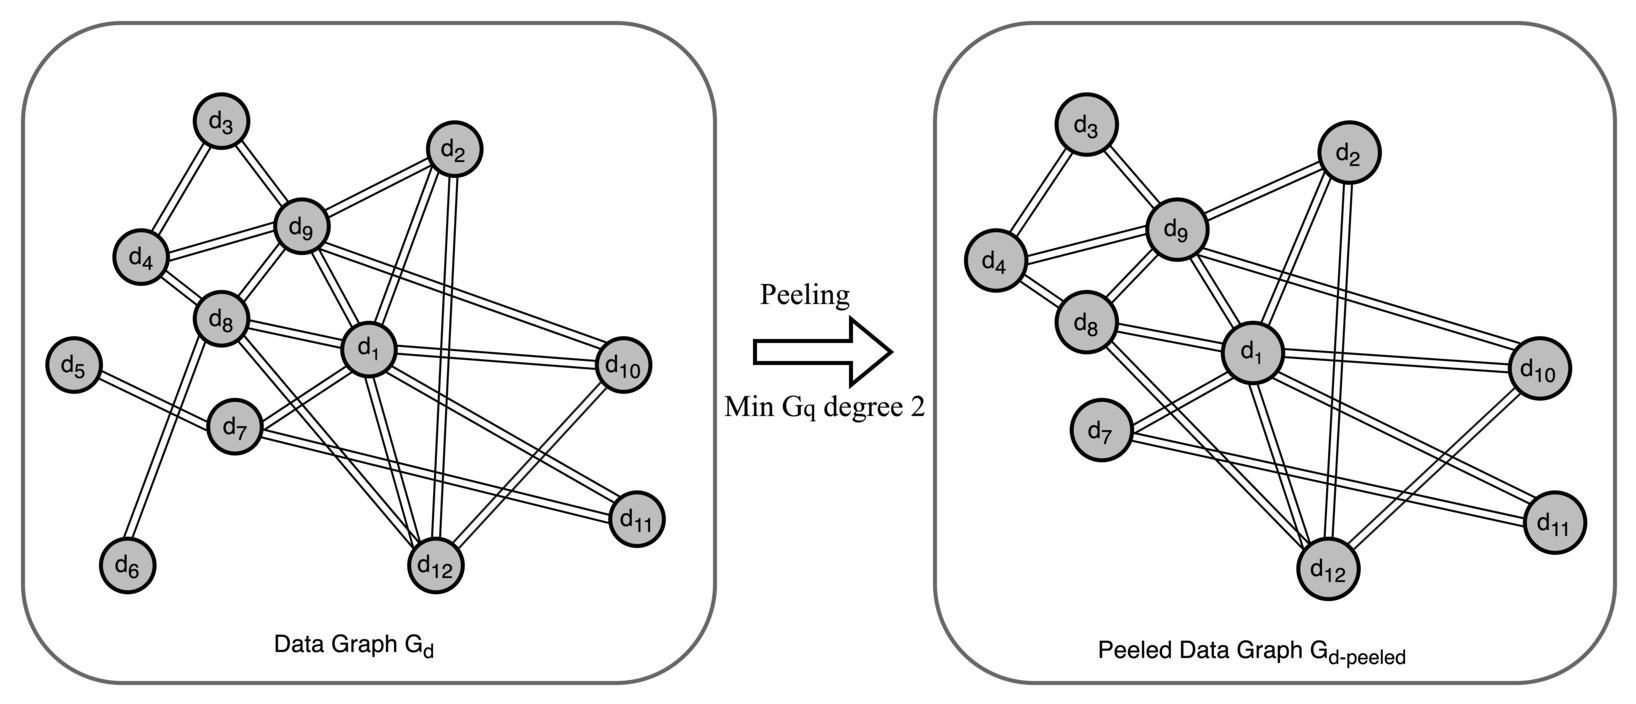
\includegraphics[width=\textwidth]{fig/LR/peeling.png}
    \caption{Peeling Example}
    \label{fig:peeling}
\end{figure}

\subsection{Priority Sorting}\label{sec:prio-sorting}
CSRCOO storage format allows efficient storage of graphs in CPU memory.
As mentioned in Section \ref{storage-format}, the \textit{Column Index} array is sorted by vertex labels to enable binary search.
However, efficient symmetry breaking demands the neighbors to be listed in a different order.
To achieve this, we need another copy of the \textit{Column Index} array in a \textit{priority} sorted fashion while maintaining the same \textit{Row Pointer} boundaries. This array is named \textit{Priority Sorted Column Index} or \textit{PSCI}.
The \textit{priority} can be any property of the vertices; in our case we explore two properties: Degree and Degeneracy.
\begin{figure}
    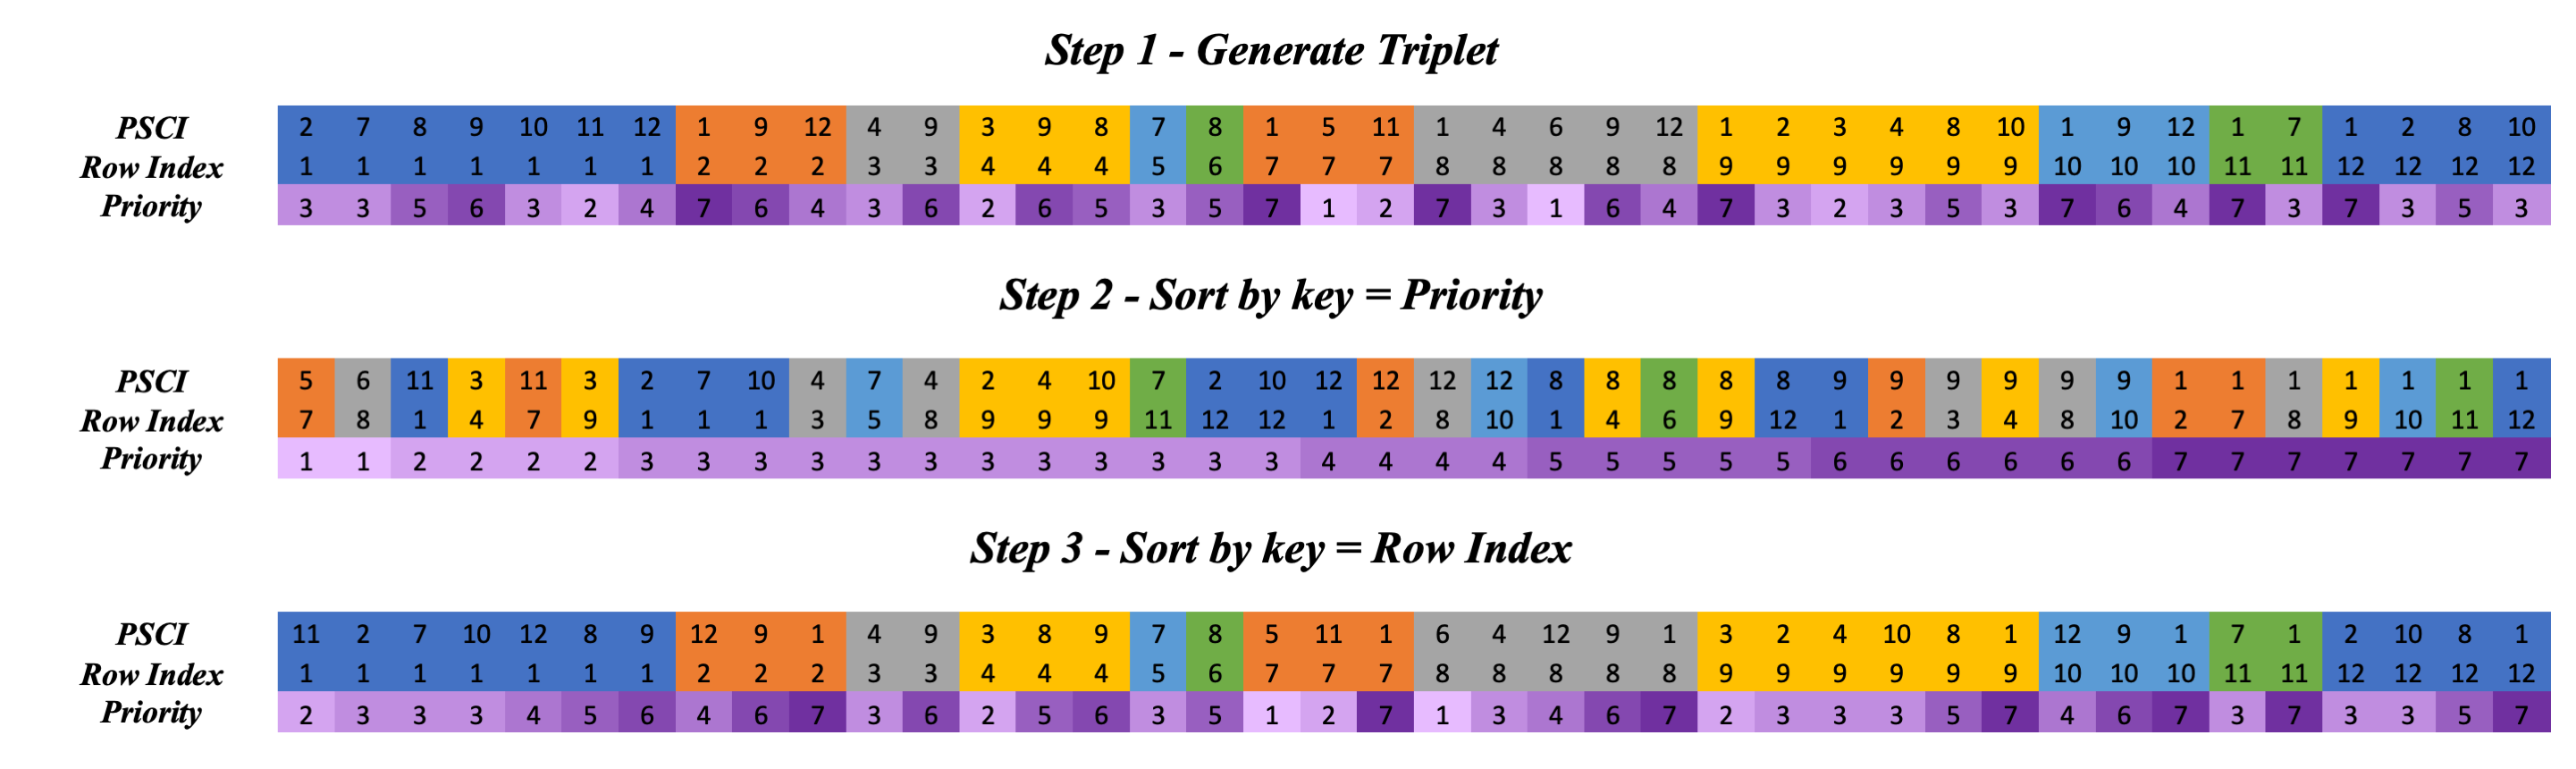
\includegraphics[width=\textwidth]{fig/LR/prio-sorting.png}
    \caption{Generating Priority Sorted Column Index Array}
    \label{fig:prio-sorting}
\end{figure}
Given the size of data graph we use GPUs for this preprocessing task.
The \textit{PSCI} array can be generated using a series of two stable sorts, since sorting is fast on GPUs this can be achieved by using the CUB library.
To start with, the \textit{PSCI} array is taken as a copy of the original \textit{Column Index} array.
An array of triplets is then created with each entry containing an element from \textit{PSCI}, \textit{Row Index}, and \textit{priority}. Where, \textit{priority} is an array with entries corresponding to the required property in \textit{PSCI}.
This array of triplets is subjected to two key based stable sorts, the first sort is with the keys being entries in the \textit{priority} array while second sort is with the keys being entries in the \textit{Row Index} array. Figure \ref{fig:prio-sorting} shows the priority sorting performed on $G_d$ as a series of key sorts.

\subsection{Induced Subgraph}\label{encoding}
The search space in the subgraph isomorphism problem is essentially the whole graph for a general query.
This makes the problem extremely challenging to scale.
However, most practical applications of subgraph isomorphism focus on dense templates.
Similar to \cite{mohammad_K-clique}, we note that restricting the search space can provide immense performance improvements, especially on the GPUs due to enhanced memory utilization.

\begin{figure}
    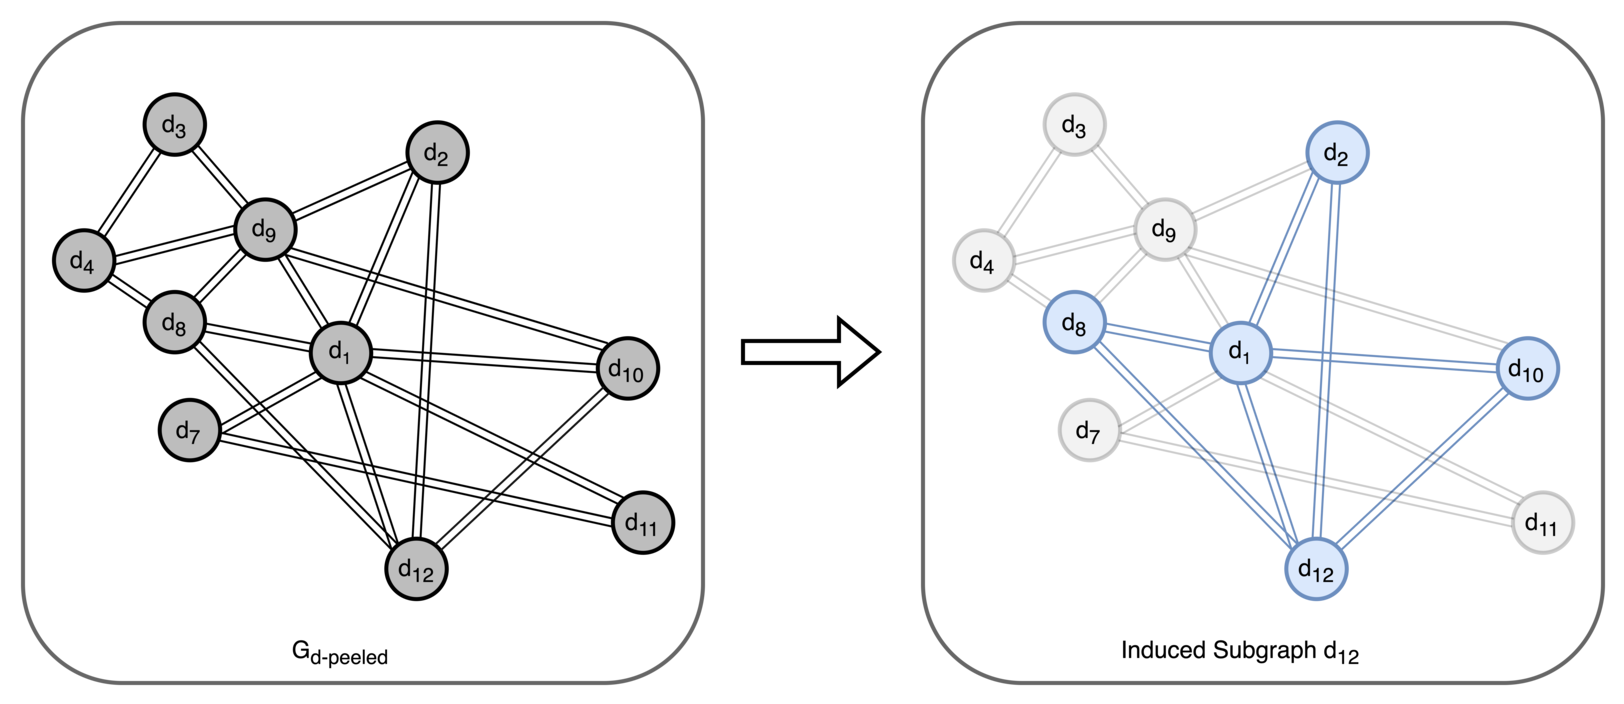
\includegraphics[width=\textwidth]{fig/LR/Induced-subgraph.png}
    \caption{Induced Subgraph for vertex $d_{12}$}
    \label{fig:induced-subgraph}
\end{figure}

The search space can be restricted by focusing on query graphs containing at least one \textit{Central node}.
A central node is defined as a node in the template graph that is connected to all other nodes.
Under the assumption of a central node, the search space for each match is limited to the subgraph induced by the data vertex matched to the central node.
Figure \ref{fig:induced-subgraph} shows the subgraph induced by vertex $d_{12}$.
To save storage space, the induced subgraph is stored in a binary adjacency matrix format.
The binary format allows fast set intersection operations as well as efficient symmetry breaking.
To use priority based symmetry breaking, the columns of the adjacency matrix are ordered with \textit{Priority Sorted Column Index} Array.

\section{Search Tree Traversal}\label{DFS-T}
% The algorithm was first developed by \cite{ullman_sgm} in $1976$.
% This was a DFS based brute force search technique that uses an adjacency matrix of size $|V_q| \times |V_d|$ as a bijection between an element in the query template and data graph.
% These matrices are recursively generated in a DFS based enumeration process to ultimately generate all the instances.
% The new candidates are generated using the conditions imposed by query graph itself.
% This algorithm assumes a directed query graph and template graph as input.
This section explains how the sequenced query graph $G_q$ and processed data graph $G_d$ are used to perform the search tree traversal for enumerating all matches.
% Let, the directed acyclic query graph be ${G}_q = (V_q, E_q)$ and the processed data graph be $G_d=(V_d, E_d)$.
% We will assume this transformation for the example given in Figure \ref{fig:sgm-example}, the post process query graph is shown in \ref{fig:query-sequencing} and data graph is shown in Figure \ref{fig:peeling}.\\

Algorithm \ref{algo:DFS-traversal} describes the DFS based iterative search tree traversal process.

\begin{algorithm}
    \caption{DFS Traversal}
    \label{algo:DFS-traversal}
    \small
    \SetKwData{l}{$l_{init}$}
    \SetKwData{isubgraph}{$G^d_{ind}$}
    \SetKwData{imatches}{$\texttt{matches}_{init}$}
    \SetKwData{isize}{$\texttt{num\_matches}_{init}$}
    \SetKwData{currIdx}{$\texttt{curr\_idx}$}
    \SetKwData{matches}{$\texttt{matches}$}
    \SetKwData{nmatches}{$\texttt{num\_matches}$}

    \SetKwFunction{intersect}{GenNextCandidates}

    \SetKwData{omatches}{$\texttt{final\_enum}$}
    \SetKwData{ocount}{$\texttt{count}$}

    \KwIn{Sequenced Query Graph: $G_q=(V_q,E_q), S_q$ \newline
        Induced Subgraph: \isubgraph. Initial level: \l \newline
        Initial set of Nodes at \l: \imatches and size \isize
    }
    \KwOut{Set of enumerated matches and count: \omatches, \ocount}
    $l \leftarrow $ \l, $\matches[l] \leftarrow $\imatches, $\nmatches[l] \leftarrow $\isize\;
    $ \currIdx \leftarrow 0$, $\omatches \leftarrow \phi $, $\ocount \leftarrow 0$  \;
    \While{$\currIdx[l] \leq \nmatches[l] $}{

        % $\matches[l+1] \leftarrow \matches[l][\currIdx[l]]$\;
        \intersect()\;
        $\nmatches[l+1]=|\matches[l+1]|$\;
        \If{$(\nmatches > 0 \textbf{ and } l < |V_q|-1$)}{
            $l\leftarrow l+1$\;
            $\currIdx[l]\leftarrow 0$\;
        }
        \ElseIf{$l==|V_q|-1$}{
            \For{$n=\l \textbf{ to } \nmatches[l+1]$}{
                $\texttt{match}\leftarrow \phi$\;
                \For{$k=\l \textbf{ to } l$}{
                    $\texttt{match} \leftarrow \texttt{match} \cup \matches[k][\currIdx[k]]$
                }
                $\omatches \leftarrow \omatches \cup \texttt{match}$
            }
            $\ocount\leftarrow \ocount + \nmatches[l+1]$
        }
        \Else{
            $\currIdx[l]\leftarrow \currIdx[l]+1$\;
            \While{$\currIdx[l]==\nmatches[l] \textbf{ and } l > \l$ }{
                $l\leftarrow l-1$\;
                $currIdx[l]\leftarrow \currIdx[l] +1 $\;
            }
        }

    }
\end{algorithm}

The whole traversal can work within a DFS stack of size $|V_q|\times Degree_{max}(G_d)$.
At each node of the search tree, \textit{GetNextNodes} function is called which generates the candidates to be visited in the next level.
This function is described in Algorithm \ref{algo:intersect}.
It performs an adjacency list intersection operation to generate all possible candidates for the next level (lines 2 - 5).
Since, there might be redundant candidates generated due to the symmetry of the query, some of them need to be pruned. This is done by the next loop (lines 6 - 8).
Note that the set $\mathcal{V}_{orient}$ is available without overheads due to the column order of the induced subgraphs.

\begin{algorithm}
    \caption{Generate Candidates for Next Level}
    \label{algo:intersect}
    \SetKwData{isubgraph}{$G^d_{ind}$}
    \SetKwData{currIdx}{$\texttt{curr\_idx}$}
    \SetKwData{matches}{$\texttt{matches}$}
    \SetKwData{nmatches}{$\texttt{num\_matches}$}
    \SetKwFunction{intersect}{GenNextCandidates}
    \KwIn{Induced Subgraph \isubgraph, level $l$ \newline
        Backward Neighbor List $\mathcal{N'}$ \newline
        Symmetry levels List $\mathcal{S}$ \newline
        Set of vertices of lower priority than given vertex $\mathcal{V}_{orient}()$ \newline
        List of matches in previous levels $\matches[]$
    }
    $\texttt{Function }\intersect() $\newline
    \While{$(\currIdx[l]<\nmatches[l])$}{
    \ForAll{$k \in \mathcal{N'}(S_q[l+1])$}{
        $u \leftarrow \matches[k][\currIdx[k]]$\;
        $\matches[l+1] \leftarrow \matches[l+1]\cap \mathcal{N}(\isubgraph(u))$\;
        }
        \ForAll{$j \in \mathcal{S}(S_q[l+1])$}{
            $u \leftarrow \matches[j]$\;
            $\matches[l+1]\leftarrow \matches[l+1] \setminus \mathcal{V}_{orient}(u)$\;
        }
    }
    $\texttt{Function End}$
\end{algorithm}

We now walk through the Search tree traversal algorithm with the example query graph sequence given in Figure \ref{fig:query-sequencing} and the peeled data graph in Figure \ref{fig:peeling}.
% Note, the pseudocode gives a DFS-based traversal tree but since it does not store the whole tree, we resort to a BFS traversal here for enumerating the whole exploration tree. \RN{language!}
Note, the pseudocode in Algorithm \ref{algo:DFS-traversal} describes a DFS-based traversal technique while the example enumerates search tree traversal in a BFS manner for illustration purposes.

\begin{enumerate}[Step 1:]
    \item Select candidates in $G_d$ with degree greater than or equal to $q_1$. Here only vertices $\{d_1, d_8, d_9, d_{12}\}$ will be selected. All these are matched to $q_1$ and traversed separately. For conciseness, we will only consider vertices $d_1$ and $d_{12}$. These matches are shown in Figure \ref{fig:sgm-step2}.
          \begin{figure}
              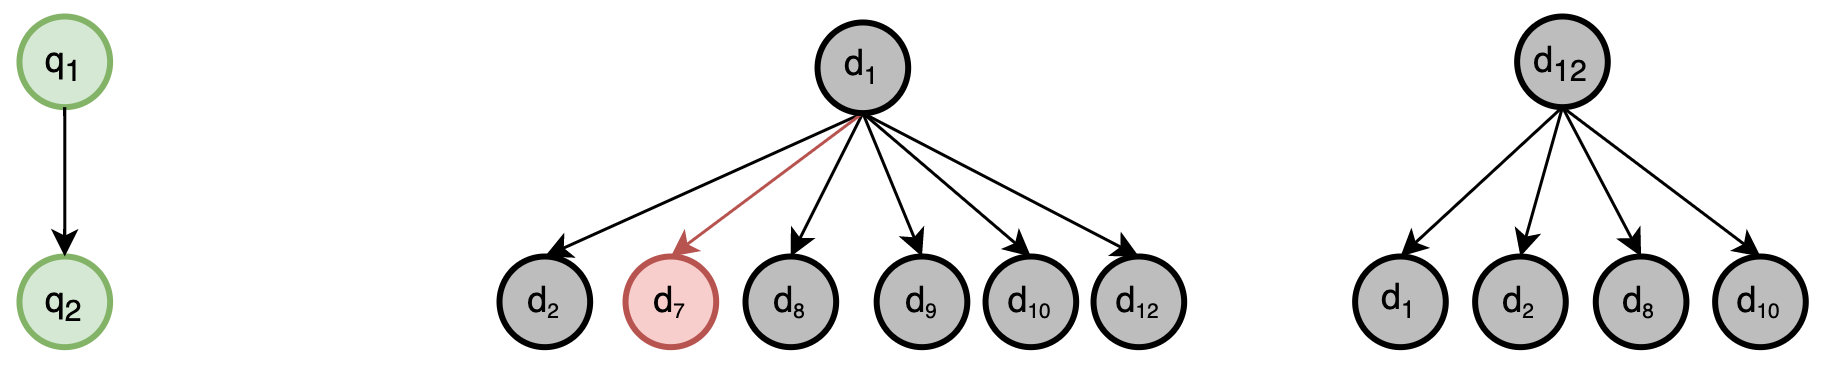
\includegraphics[width=\textwidth]{fig/LR/sgm-step2.png}
              \caption{Step 1}
              \label{fig:sgm-step2}
          \end{figure}
    \item For candidates of level 2, select all neighbors of vertex matched at level 1 with degree greater than that of $q_2$, i.e., 3. As shown in Figure\ \ref{fig:sgm-step3} for the subtree rooted at $d_1$, there will be 5 candidates: $\{d_2, d_7, d_8, d_9, d_{10}, d_{12}\}$. Out of these 5 candidates, $d_7$ is pruned since, it has degree less than $q_2$.\\
          \begin{figure}
              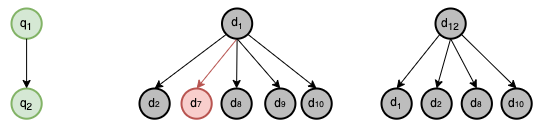
\includegraphics[width=\textwidth]{fig/LR/sgm-step3.png}
              \caption{Step 2}
              \label{fig:sgm-step3}
          \end{figure}
          For subtree rooted at $d_{12}$, there will be 4 candidates: $\{d_1, d_2, d_8, d_{10}\}$ and none can be pruned.
    \item Level 3 candidates are obtained by the intersection of matches at level 2 and level 1. Since this level is symmetric to level 2 symmetry breaking needs to be performed. We use the decreasing degree criteria for symmetry breaking in this example. This can be performed without any overheads since the nodes are stored in desired priority order in \textit{PSCI}.
          \begin{figure}
              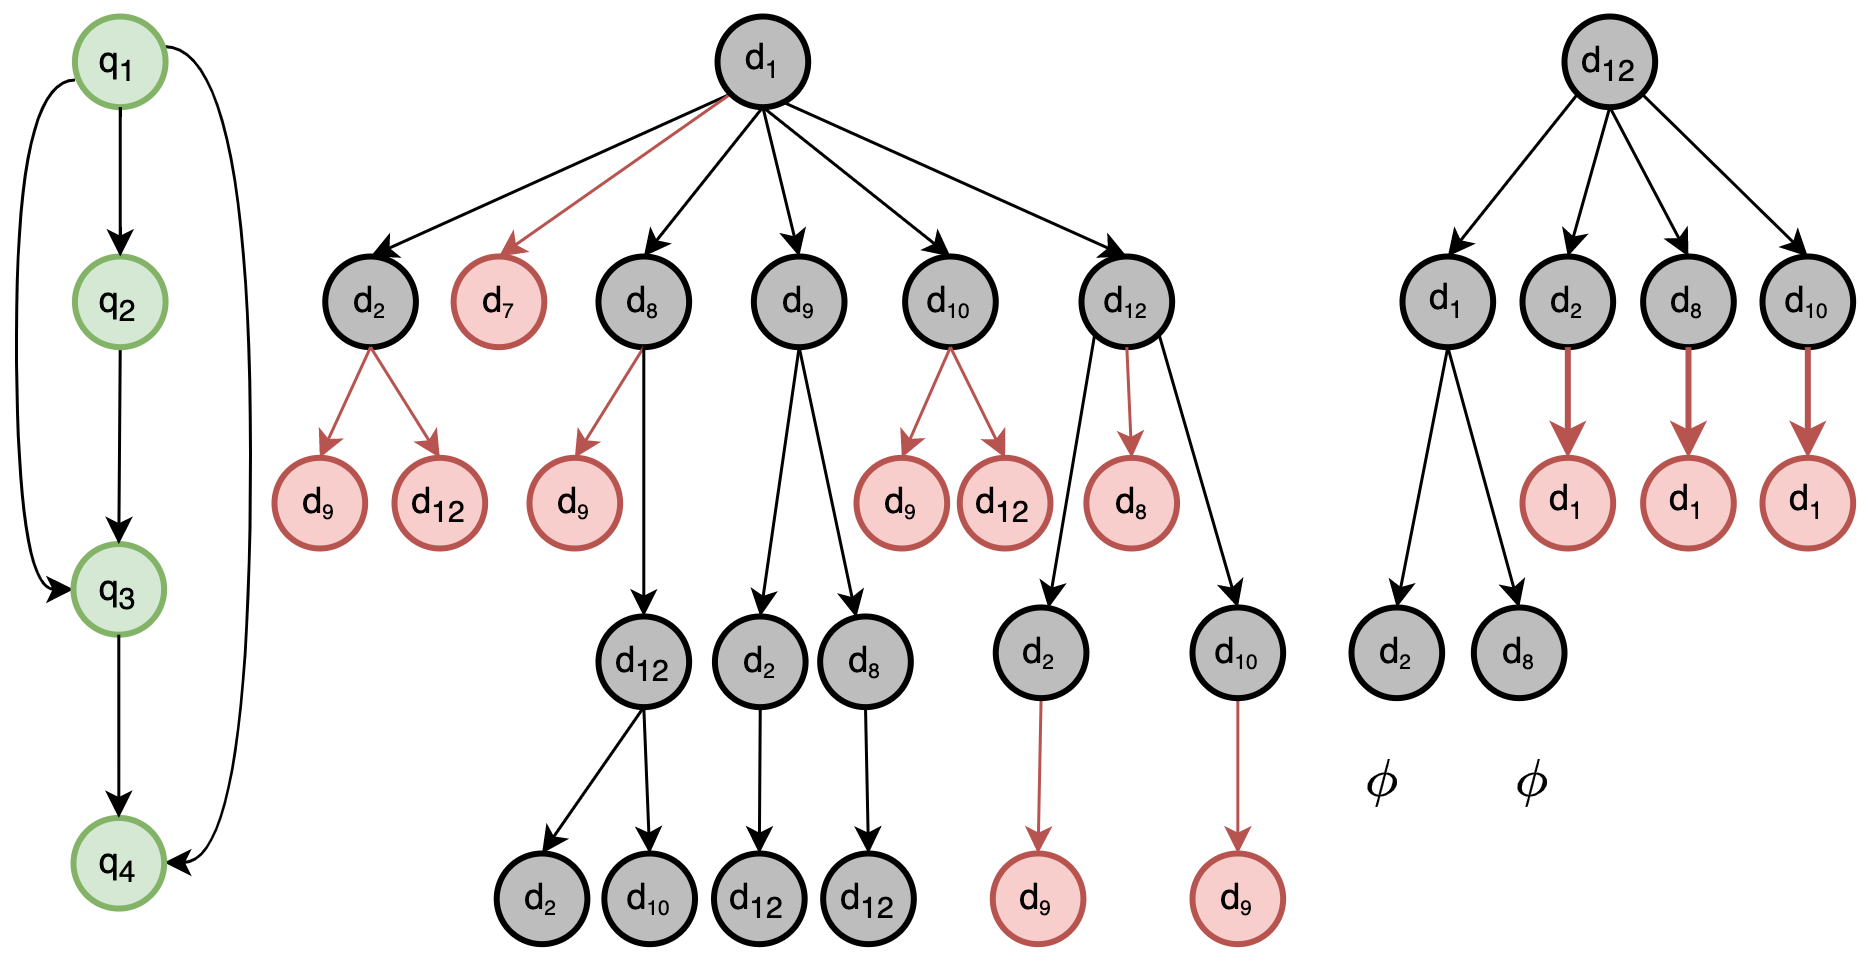
\includegraphics[width=\textwidth]{fig/LR/sgm-step4.png}
              \caption{Step 3}
              \label{fig:sgm-step4}
          \end{figure}
          Figure \ref{fig:sgm-step4} shows all candidates at level 3. The candidates marked in red are pruned.
          For example 9 and 12 is pruned in subtree ${d_1, d_8, \dots}$ since $Degree(d_9)<Degree(d_8)$.
    \item For level 4 candidates, the adjacency intersection of $q_1$ and $q_3$ is required. This level is also symmetric to level 2. The subtree rooted at $d_{12}$ does not yield any candidates. While the other gets one candidate each. Symmetry Breaking does not prune any candidates here.
          \begin{figure}
              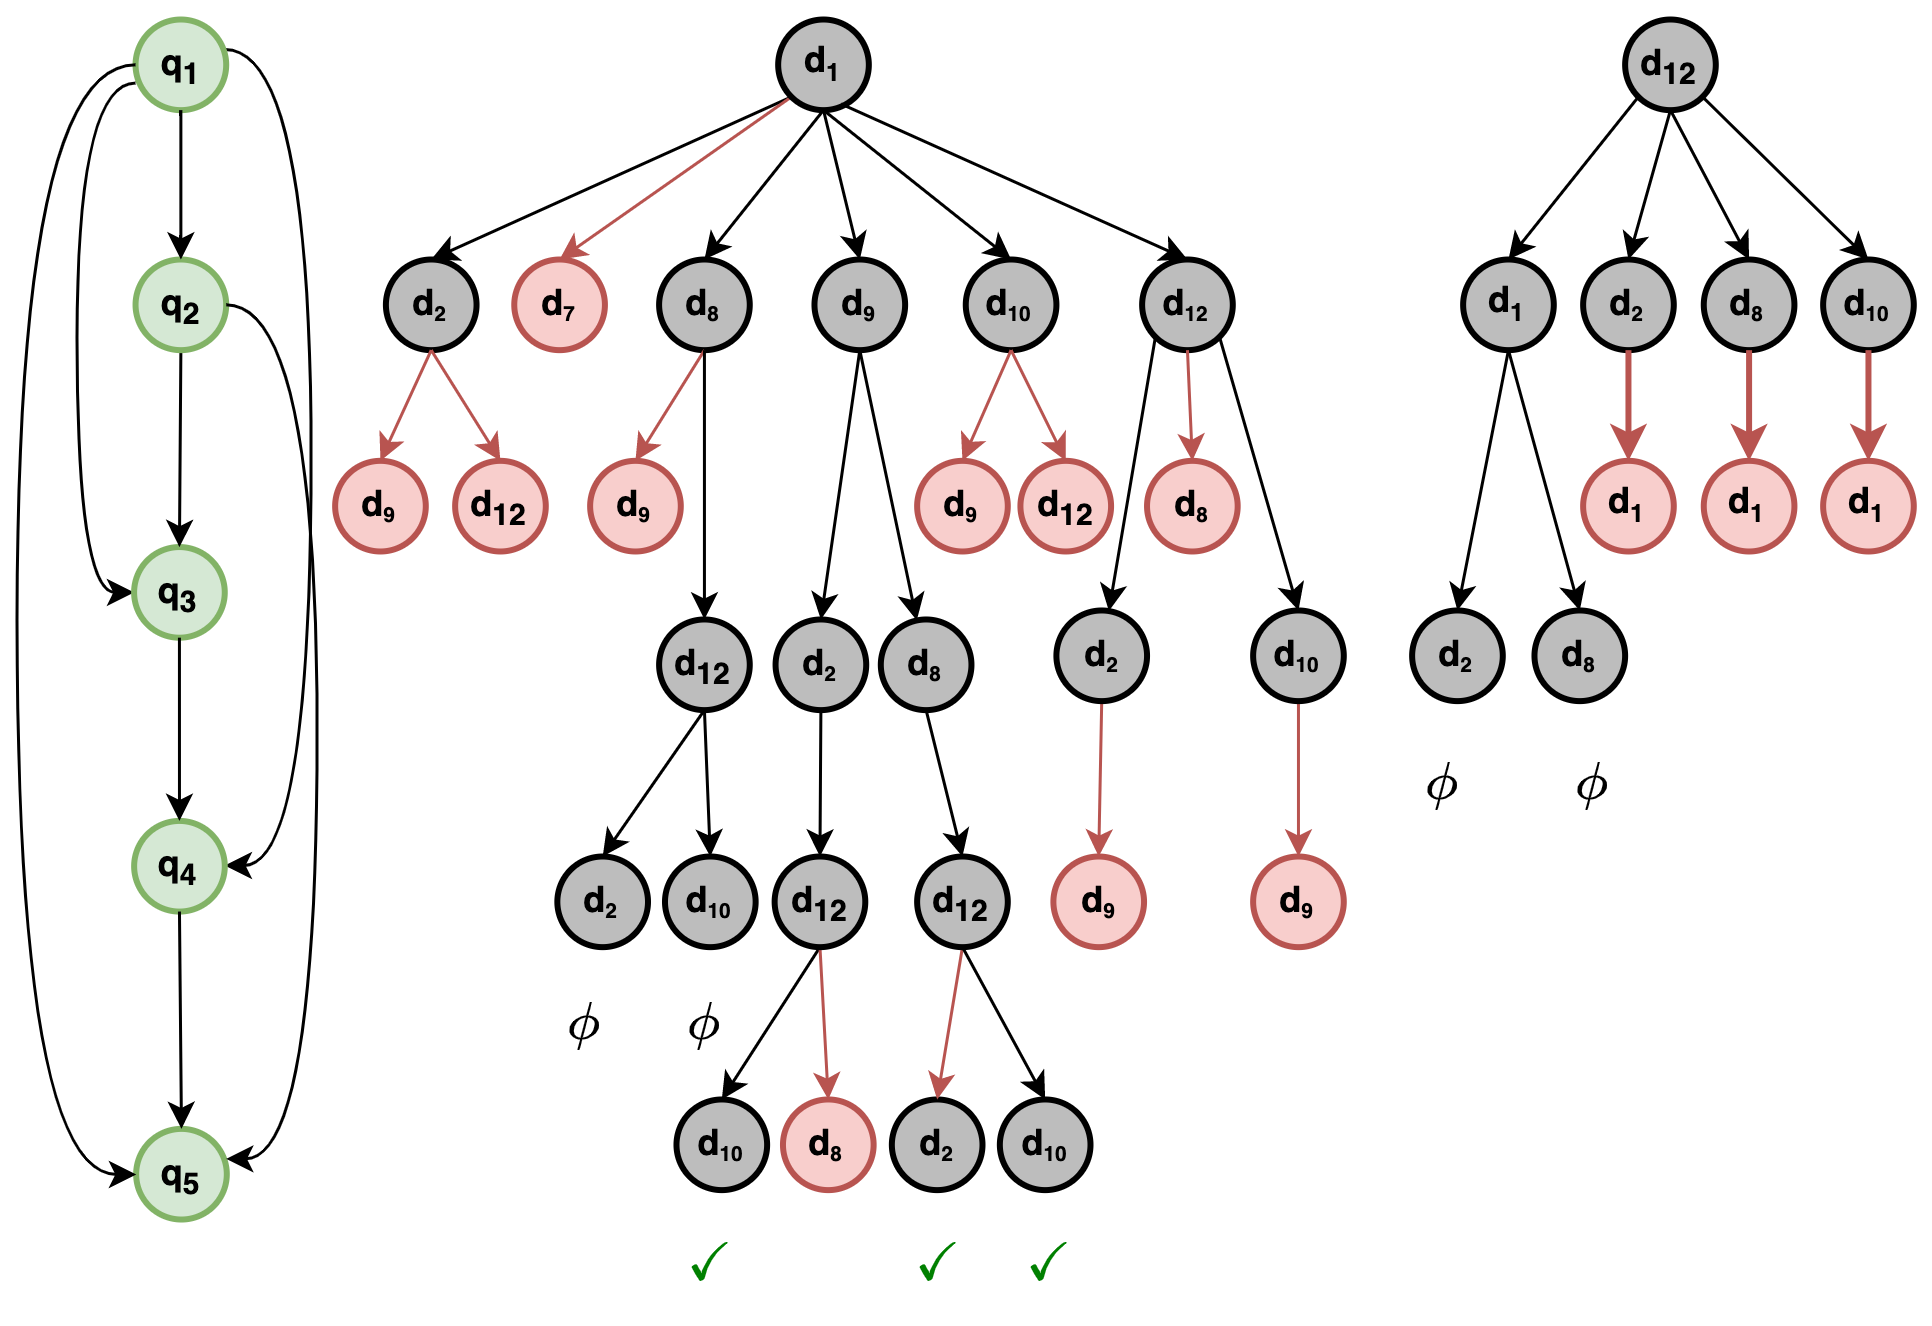
\includegraphics[width=\textwidth]{fig/LR/sgm-step5.png}
              \caption{Step 4}
              \label{fig:sgm-step5}
          \end{figure}
    \item Level 5 candidates (or final matches) are generated by the adjacency intersection $q_1$, $q_2$, and $q_4$. This level is symmetric to both $q_2$ and $q_3$.
          The candidates generated by intersection at the first leg are $\{d_8, d_{10}\}$, symmetry breaking will eliminate both the candidates as $Degree(d_2)<Degree(d_8)$. \RN{DONE TILL HERE.} There is a tie between $d_2$ and $d_{10}$ which is resolved \textit{lexicographically}.
          \begin{figure}
              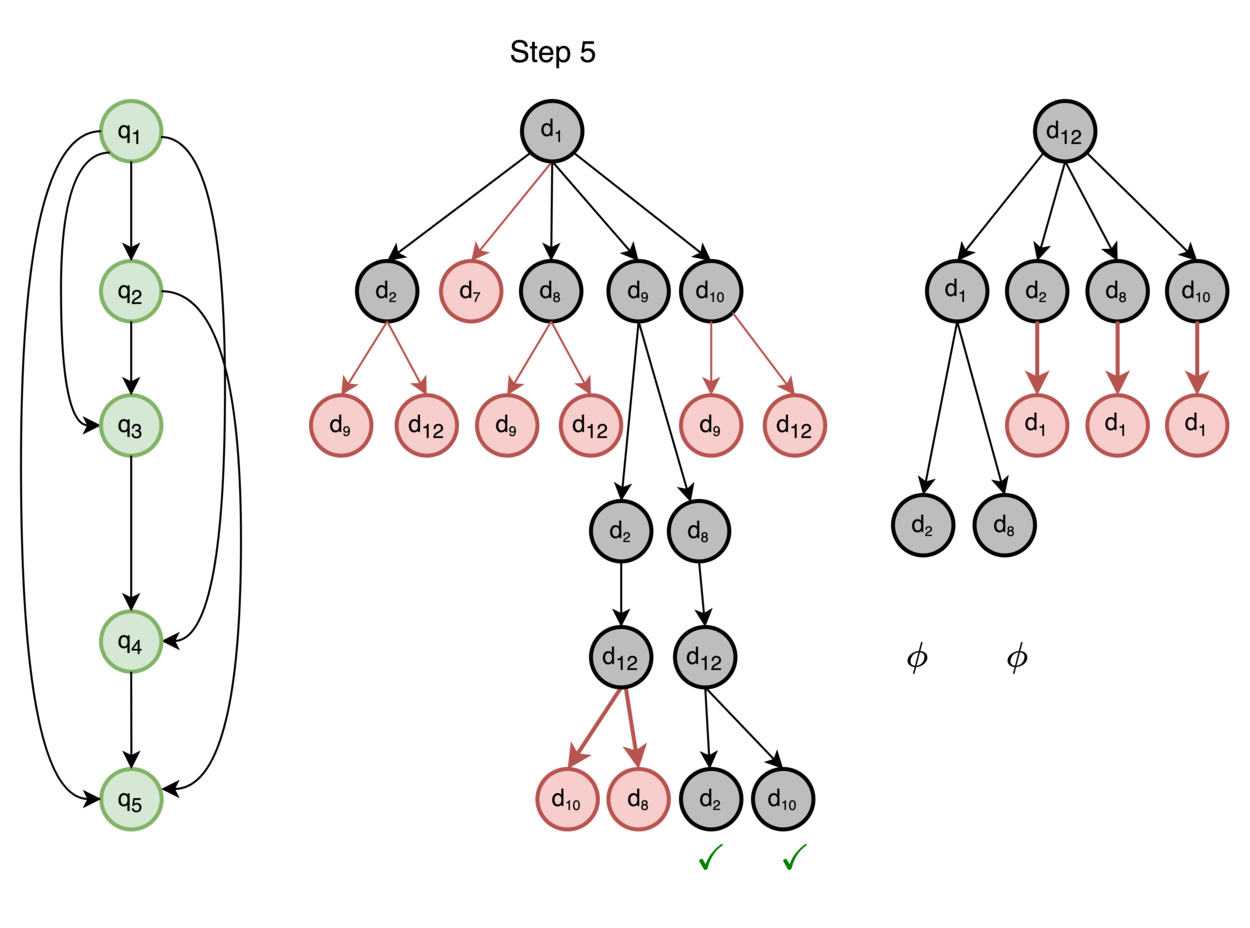
\includegraphics[width=\textwidth]{fig/LR/sgm-step6.png}
              \caption{Step 5}
              \label{fig:sgm-step6}
          \end{figure}
          Similarly, the other leg generates 2 valid candidates for level 5.
\end{enumerate}
This way the search tree traversal process terminates with final matches
$\{d_1, d_9, d_8, d_{12}, d_2\}$ and $\{d_1, d_9, d_8, d_{12}, d_{10}\}$.
There might be more matches originating from subtrees rooted at $\{d_8, d_9\}$ which were not illustrated here.

To conclude, this chapter gives a detailed understanding of all techniques involved in subgraph enumeration. As we can see, all subtrees are independent of each other hence, they can be trivially parallelized on GPUs by allocating a block to each of these subtrees.

One more subtle observation to be made here is that the exploration is dependent on the symmetry breaking technique.
We can see from Figure \ref{fig:sgm-step4} that there would have been many more candidates at level 4 if the symmetry breaking was done using lexicographic criteria or increasing degree criteria.
These candidates would have ultimately pruned in lower levels, resulting in extra work.
Therefore, selecting an efficient symmetry-breaking strategy is important and discussed in detail later in Section \ref{sec:hy-symbreak}.

\chapter{Improvements}{\label{chap:Improvements}
Multiple ideas were applied to improve the performance of baseline, PARSEC \cite{PARSEC_VD}, this section lists each idea and its individual impact on performance.
All improvements are then combined to present final improvement results in Chapter \ref{chap:Results}.
The basic philosophy is to find the most time-consuming step and try to make it faster using algorithmic or computational techniques.

The criteria used for quantifying the contributions of these improvements are number of intersections and runtime.
These numbers are reported as speedups, the ratio of old to new.
Formally, we define the intersection speedup and time speedup as:
$$
    \text{Intersection Speedup} = \frac{\text{\# of Intersections Baseline}}{\text{\# of Intersections New}}
$$
$$
    \text{Time Speedup} = \frac{\text{Run time Baseline}}{\text{Run time New}}
$$
The information of data graphs and queries used to report individual performance impact is mentioned in Section \ref{sec:expt-info}.

\section{Intersection Reuse}\label{sec:reuse-impl}
Set intersection operation for generating candidates at the next level is the most time-consuming operation in subgraph enumeration, this is a well-established fact in the literature \cite{RPS-paper}, \cite{LIGHT}, \cite{VF3}.
This was also verified for the baseline \cite{PARSEC_VD}. Figure \ref{fig:time-dist} gives the distribution of time spent by each operation in different tasks. The Intersect operation shown here is the time taken by Algorithm \ref{algo:intersect}.
\begin{figure}
    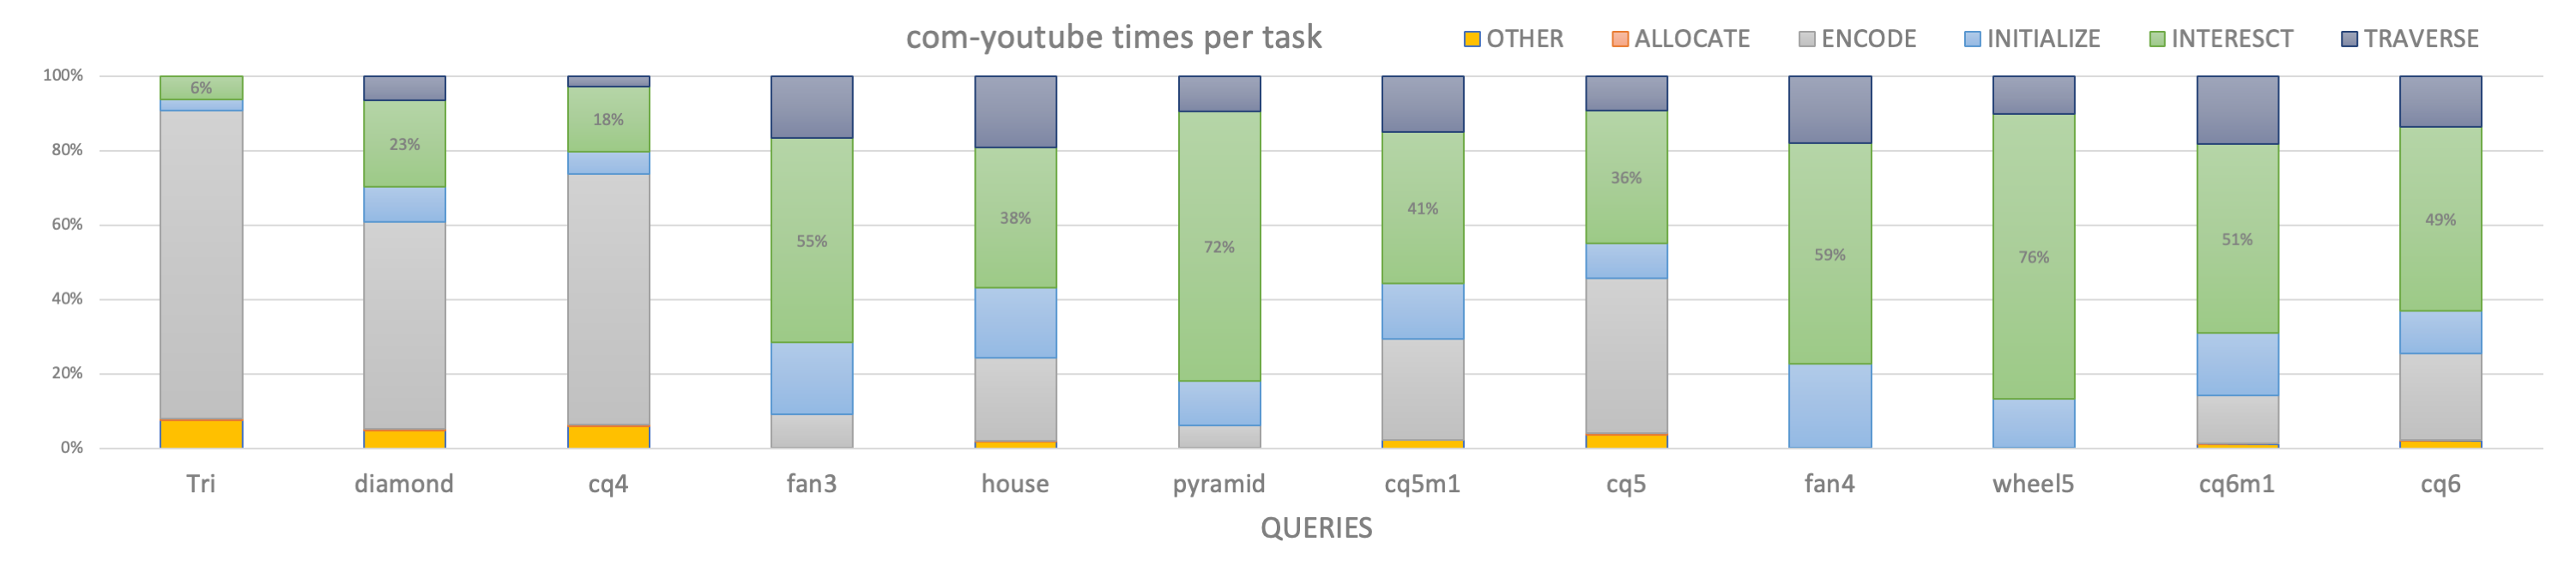
\includegraphics[width=\textwidth]{fig/improvements/time-distributions-yt.png}
    \caption{Stepwise Fraction Time spent}
    \label{fig:time-dist}
\end{figure}
This algorithm involves iterating over each element of the backward element list to perform intersection and generate possible candidates for next level (lines 2 - 5).
The number of backward neighbors at each level increases with increasing template size. This results in even more adjacency list intersections at each level.
RPS \cite{RPS-paper} reduces these operations by generating an intersection reuse plan, this plan smartly finds the intersections that will be required by more than one node and stores them when first calculated. There is a lot of intersection reuse possible with RPS as they employ a BFS strategy.
Similar extent of reuse is not possible in DFS traversal since the past information is lost while backtracking.
However, Some levels of the sequenced query graphs have similar backward neighbor lists. For such queries, the majority of intersections can be reused by simply storing the intermediate intersection results.
To do this efficiently, one needs to match levels with similar adjacency lists. This problem is posed as a linear programming optimization problem.

Let, the sequenced query graph be $G_q=(V_q, E_q)$ with $|V_q|=k$ and the vertex sequence $S_q$.
$\mathcal{N}(.)$ be the function for getting the backward neighbor list of a vertex.
For each pair of vertices at level $i$ and $j$ let $W_{ij}$ be a measure of the commonality between their backward neighbors' lists. Let $X_{i,j}$ be the decision variable which tells if vertex $i$ should reuse intersections from vertex $j$.

With these definitions the optimization problem can be modelled as:
\begin{align}
    \max \sum_{i=j+1}^{k}\sum_{j=1}^{k} W_{ij} X_{ij} \\
    \text{s.t.}
    \sum_{j=1}^k X_{ij} \leq 1. \quad \forall i \in \{1, \dots, k\}
\end{align}
Where, $$
    W_{ij} = \begin{cases}
        |\mathcal{N}(S_q[i]) \cap \mathcal{N}(S_q[j])| \qquad \text{if} \quad i>j, \mathcal{N}(S_q[i]) \supseteq \mathcal{N}(S_q[j]) \\
        0   \qquad \text{Otherwise}
    \end{cases}
$$
This problem is a linear semi-assignment problem (LSAP) with the greedy solution being optimal.
This is easy to establish as any other solution can be improved by switching to the greedy solution.
The solution to this problem is:
$$
    X_{ij}=\begin{cases}
        1   \qquad \text{if } j=\argmax_j(w_{ij}>0); \\
        0   \qquad \text{Otherwise}
    \end{cases}
$$
Reuse detection involves a find minimum operation for each level in $G_q$ hence it is polynomial time and can be performed on CPU for small-sized query graphs.
The mappings found $x_{ij = 1}$ implies that level $i$ can use intersection results from level $j$.
Hence, the level $j$ is flagged as \textit{reusable} and its results are stored along with the DFS stack.
Algorithm \ref{algo:reuse} lists the reuse detection and post-processing recipe.
To save on constant memory the query graphs are stored in CSR format.
After finding the reuse mappings from the query, the column index of $(G_q)$ needs to be modified for the search tree traversal step to utilize this information.
The modification step involves reordering the lists and generating the reuse pointer array.

We show reuse detection at work on the example query in Figure \ref{fig:sgm-example}.
Here, only $w_{54}$ and $w_{53}$ are positive with value 2. Hence, any of the levels 3 or 4 can be marked reusable, Let's assume level 4.
The backward neighbors of level four are $\{1,3\}$ and for level five they are $\{1,2,3\}$. To avoid checks in the for loop of Algorithm \ref{algo:intersect} line (2).
Another Reuse pointer array is created which gives the start of the remaining neighbors of level 5.

\begin{figure}
    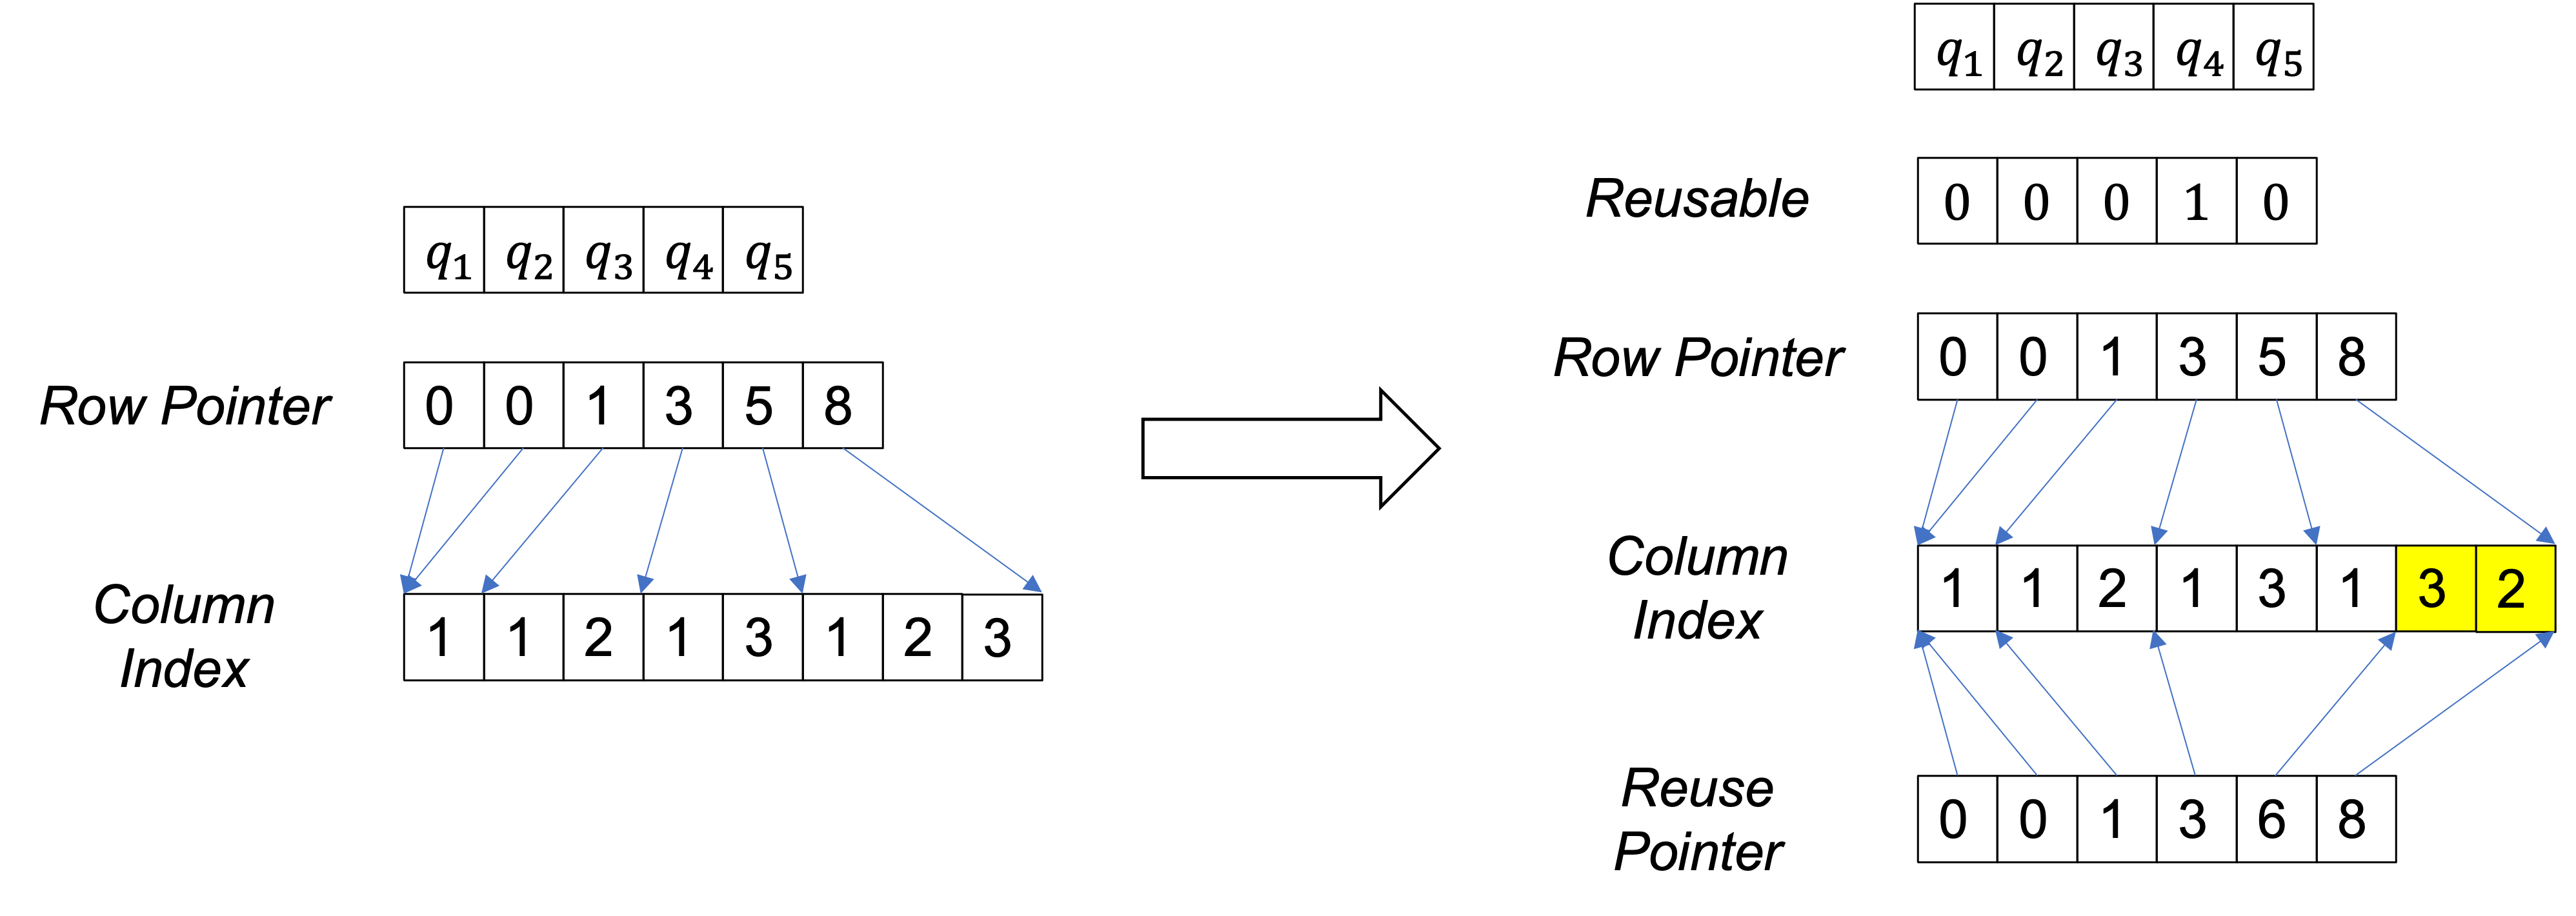
\includegraphics[width=\textwidth]{fig/improvements/Reuse-resorting.png}
    \caption{Reuse Detection Example}
    \label{fig:reuse-detection}
\end{figure}
Once the reuse is detected and pointers set, this data is sent to the GPU constant memory for the rest of the application. For implementing reuse, the function in Algorithm \ref{algo:intersect} needs to be changed to add conditions for checking if a level is reusable or if the reuse pointer is updated. This is shown as a flow chart in Figure \ref{fig:reuse-flowchart}.
\begin{figure}
    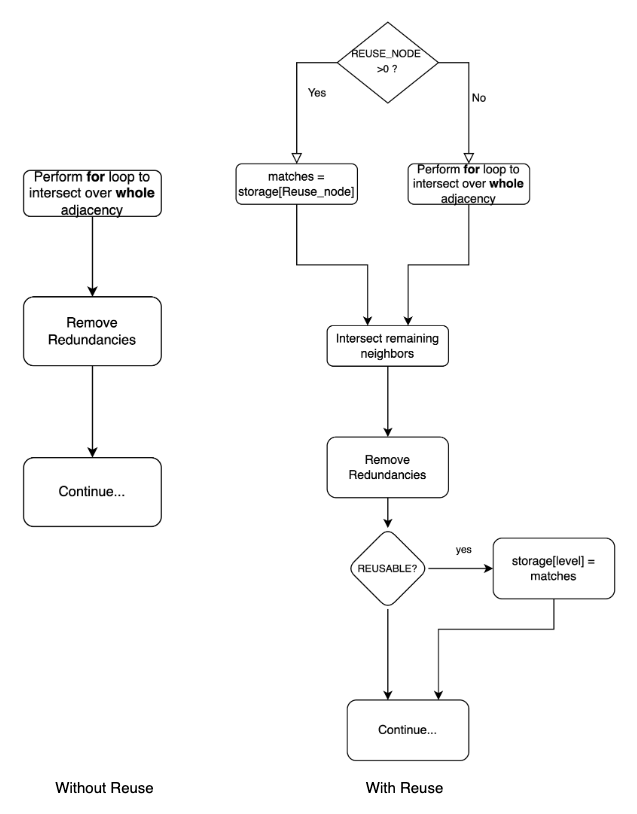
\includegraphics[width=\textwidth]{fig/improvements/reuse-flow.png}
    \caption{Flowchart with and without reuse}
    \label{fig:reuse-flowchart}
\end{figure}
This way, reuse reduces computational workload and adds to the memory workload.
Since global memory writes are relatively expensive, some shared memory can be utilized to write the intermediate intersection results while longer results can be spilled to global memory.

\begin{algorithm}
    \caption{Reuse Detection}
    \label{algo:reuse}
    \SetKwData{qgraph}{$G_q=(V_q, E_q)$}
    \SetKwData{bneighbor}{$\mathcal{N}(V_q)$}
    \SetKwData{reusable}{$\texttt{reusable}$}
    \KwIn{Directed Query Graph \qgraph \newline
        Arrray of Backward Neighbor lists \bneighbor
    }
    $W \leftarrow: [|V_q|][|V_q|]$\;
    $X \leftarrow: [|V_q|][|V_q|]$\;
    \reusable $\leftarrow: [|V_q|]$\;
    \ForAll{$j \in V_q$}{
        \For{$i=j+1 \textbf{ to } |V_q|$}{
            \leIf{$\bneighbor[i] \supseteq \bneighbor[j]$}{
                $W[i][j] \leftarrow |\bneighbor[i] \cap \bneighbor[j]|$\;
            }
            {
                $W[i][j] \leftarrow 0$
            }
        }
    }
    $\reusable[j] \leftarrow (\max({W[i].)} > 0)$\;
    \ForAll{$i \in V_q$}{
        \For{$j=1 \textbf{ to } i$}{
            \leIf(){$j==\argmax_j(W[i]. > 0)$}{$1$\; $\reusable[j]=1$\;}{0}
        }
    }
    \CommentSty{\texttt{// Update Reuse Pointers from $X[i][j]$}}
\end{algorithm}

The improvements due to intersection reuse are measured in terms of the number of intersections performed.
Since there are increased reads and writes to global memory the time benefit from this technique is negligible. Table \ref{tab:reuse-improvement} shows the improvement in the number of intersections with this technique.
Since the backward neighbor lists are small for sparse queries there is not much benefit due to intersection reuse.
The intersection counts also include the additional read and write operations needed due to intersection reuse.

\begin{table}[tbp]
    \centering
    % \resizebox{\textwidth}{!}{%
    \begin{tabular}{c|rrc}
        \hline
        Query                                                                  & \begin{tabular}[r]{@{}r@{}}\#Intersections  \\w/o Reuse  \end{tabular} &
        \begin{tabular}[r]{@{}r@{}} \#Intersections \\with Reuse \end{tabular} &
        \begin{tabular}[r]{@{}r@{}} Intersection \\Speedup     \end{tabular}                                                                                                 \\ \hline
        diamond                                                                & 9,722,143                                                              & 9,722,143   & 1.00 \\
        cq4                                                                    & 6,028,832                                                              & 6,028,832   & 1.00 \\
        cq5\_m1                                                                & 46,794,486                                                             & 26,360,303  & 1.78 \\
        cq5                                                                    & 20,881,838                                                             & 15,889,824  & 1.31 \\
        cq6\_m1                                                                & 130,114,516                                                            & 52,225,436  & 2.49 \\
        cq6                                                                    & 49,618,729                                                             & 30,194,042  & 1.64 \\
        cq7\_m1                                                                & 253,215,589                                                            & 81,007,445  & 3.13 \\
        cq7                                                                    & 91,679,280                                                             & 46,935,236  & 1.95 \\
        cq8\_m1                                                                & 370,669,539                                                            & 102,639,103 & 3.61 \\
        cq8                                                                    & 139,279,024                                                            & 62,709,660  & 2.22 \\
        cq9\_m1                                                                & 430,334,955                                                            & 111,122,133 & 3.87 \\
        cq9                                                                    & 181,479,780                                                            & 74,663,152  & 2.43 \\
    \end{tabular}%
    % }
    \caption{Number of intersections with and without reuse for com-youtube}
    \label{tab:reuse-improvement}
\end{table}

\section{Hybrid Symmetry Breaking}\label{sec:hy-symbreak}
Symmetry breaking is an important operation in the search tree traversal.
\cite{ullman_sgm} gives a simple ordering technique for symmetry breaking, but the criteria for this ordering is not well-defined.
It is okay to use any criteria for correctness, but good criteria can significantly improve performance.
Handling symmetries to reduce the search space is an active area of research.
The problem of finding an efficient symmetry breaking technique was shown to be strongly NP hard by \cite{crawford-sb-np-hard}.
A lot of symmetry breaking criteria have been defined since then. Most of these have linear time complexity or work only with BFS traversal.
In  the optimization domain, this problem has also been formulated as a Constraint Satisfaction Problem (CSP) but it also works only when the tree traversal is done in BFS fashion \cite{sb-CSP}.
The near-linear time complexity for each decision, constraints to perform BFS, and data sharing between subtrees make efficient symmetry breaking difficult on GPUs with DFS strategy.
Since the knowledge of \textit{global} characteristics is limited during enumeration, we resort to static characteristics like Degree and Degeneracy.
The priority sorted column index array (PSCI) (discussed in Section \ref{sec:prio-sorting}) is used to further reduce global memory accesses.

With PSCI, different symmetry breaking criteria were tried and compared to the baseline \cite{PARSEC_VD}. The baseline criteria are based on degree for level 1 and lexicographic for level 2 onwards.

The symmetry breaking performance is determined by finding the total number of intersections.
On performing these experiments, the Degeneracy based symmetry breaking seemed to perform worse than baseline across all graphs.
For degree, increasing degree based criteria seemed to perform better for some queries while decreasing criteria performed better for others.
Table \ref{tab:degree-sb} shows the Intersection speedups for the \textit{soc-pokec} and \textit{cit-patents} data graphs.
% On further analysis it was found that the templates for which decreasing ordering works better mostly had second-level asymmetric to first.

\begin{table}[h]
    \centering
    \resizebox{\textwidth}{!}{
        \begin{tabular}{r|cccccccccc}
            \hline
            \textbf{soc-pokec}   &
            Tri                  &
            Diamond              &
            Cq4                  &
            Cq5m1                &
            Cq5                  &
            House                &
            Pyramid              &
            Fan3                 &
            Cq6m1                &
            Cq6                                                                                                 \\\hline
            \textbf{Decreasing}  &
            1.22                 &
            0.53                 &
            0.66                 &
            0.89                 &
            1.19                 &
            1.49                 &
            1.88                 &
            1.76                 &
            1.06                 &
            1.41                                                                                                \\
            \textbf{Increasing}  &
            3.00                 &
            1.08                 &
            1.47                 &
            1.67                 &
            2.29                 &
            2.85                 &
            0.22                 &
            0.20                 &
            1.64                 &
            2.25                                                                                                \\
            \\
            \hline
            \textbf{cit-patents} & Tri  & Diamond & cq4  & cq5m1 & cq5  & house & pyramid & fan3 & cq6m1 & cq6  \\\hline
            \textbf{Decreasing}  & 1.22 & 0.82    & 1.24 & 2.32  & 2.91 & 4.29  & 3.15    & 3.92 & 2.51  & 3.15 \\
            \textbf{Increasing}  & 3.00 & 1.27    & 1.79 & 3.50  & 4.28 & 6.60  & 1.26    & 1.83 & 2.72  & 3.71
        \end{tabular}
    }

    \caption{Intersection Speedup with Degree based Symmetry Breaking}
    \label{tab:degree-sb}
\end{table}


Recall from \ref{sec:sym-detection} that the symmetry breaking criteria can be different for different levels and maybe different for different subtrees.
To precisely find out when it can be different and when it cannot, we present the following observation:
\begin{theorem} \label{thm:hybrid-sb}
    Symmetry breaking is independent across subtrees for central node queries with first symmetric level greater than two
\end{theorem}
\begin{proof}
    Let, the data graph be $G=(V, E)$ and $\{v_1, v_2\} \in V$. $G_{ind}(v)$ be subgraph induced by $v$ in $G$.
    % Vertex set of a graph is represented by $\mathcal{V}(.)$, the Edge set by $\mathcal{E}(.)$ the adjacency list of a vertex is represented by $\mathcal{N}(.)$ and 
    The backward neighbors list of a vertex is represented by $\mathcal{N}'(.)$.

    The proof is obvious if $\mathcal{E}(G_{ind}(v_1)) \cap \mathcal{E}(G_{ind}(v_2)) = \phi $

    If not $ \forall ~ e(x,y) \in \mathcal{E}(G_{ind}(v_1)) \cap \mathcal{E}(G_{ind}(v_2))$:

    Since, $(x,y) \in \mathcal{E}(G_{ind}(v_1)) ~ \Rightarrow ~ \{x,y\} \in \mathcal{N}(v_1)$

    Similarly,  $\{x,y\} \in \mathcal{N}(v_2)$

    Now for Algorithm \ref{algo:DFS-traversal} since level 2 vertex (say $q_2$) in the query graph is not symmetric to the level 1 vertex (say $q_1$), candidates for level 2 will be given by $\mathcal{N'}(q_2)$ where $q_2$ is the query vertex at level 2.

    Since, $q_1$ has to be a central node, $\mathcal{N'}(q_2)=q_1 \Rightarrow $ Level 2 candidates for tree rooted at $v_1$ will be $\mathcal{N}(v_1)$ and for tree rooted at $v_2$ they will be $\mathcal{N}(v_2).$

    This implies, the level $2$ candidates are independent of the symmetry breaking strategy, the edge $(x,y)$ is always considered for exploration by Algorithm \ref{algo:DFS-traversal}.

    Since, all edges in the intersection are considered independent of the symmetry breaking strategy. Each subtree will enumerate the correct number of query instances.
\end{proof}

Theorem \ref{thm:hybrid-sb} enables different symmetry breaking strategies for different subtrees. Table \ref{tab:degree-sb} shows which strategy to choose really depends on the data graph and query graph. The optimal strategy may even be different for distinct subtrees in the same data graph. To curb this variability in strategy decisions, a dynamic two phase traversal technique is designed:
The first phase is to determine if a particular subtree should perform increasing or decreasing symmetry breaking.
The second phase is to use the predetermined strategy to perform the search tree traversal.
Performing increasing or decreasing symmetry breaking differs by one step hence the second phase can simply check the predetermined strategy and prune accordingly.

For phase 1, the problem of finding an optimal strategy is strongly NP hard. Thus, any practical implementation can only develop Heuristics.
A natural strategy to decide the strategy in phase 1 might seem to be based on counting the number of eligible candidates till first symmetric level. This does not work as both strategies will produce same number of candidates.
% This hints that there should be a criterion to determine the \textit{quality} of these candidates.
This hints at designing a criterion to determine the \textit{quality} of these candidates.
Since the candidates generated are sorted by priority, we use the following observations to determine their \textit{quality}:
\begin{enumerate}[Obs1:]
    \item For increasing symmetry breaking, the left side of the DFS subtree has lesser candidates (vice versa for decreasing).
    \item Few candidates on the left side may generate more nodes in subsequent levels, while the right side candidates (high count) might not.
\end{enumerate}
So the weights should be selected based on an equalizing philosophy where higher weight is given to the left side of the tree (for increasing) and less to the right side.
Candidate wise increasing weights based on index of the candidate and the total number of candidates is chosen for this purpose.

To formalize, Let the total number of candidates at $j^{th}$ leaf in the subtree be $C_j$ and the total number of enumerations found till this level be $S$.
The symmetry breaking strategy is determined based on the weighted sum (say $WS$).
$$WS = \sum_j C_j\times W_j$$
The weightage $W_j$ for the quality of this branch is given by:
$$
    W_j=\begin{cases}
        (S - j) \qquad \text{for increasing} \\
        j \qquad \text{for decreasing};
    \end{cases}
$$
The strategy is chosen for subtrees based on whichever weighted sum $(WS)$ is smaller.

To find the efficiency of this strategy, we compare it with the best, worst, and pure strategies using intersection speedup criteria.
Table \ref{tab:hybrid-symbreak-performance} shows that hybrid strategy often works better than pure strategy and is sometimes close to the best possible strategy.
This improvement in reduced work reflects in time improvements.
Table \ref{tab:speedups-hy-sym} gives the time speedups for \textit{fan3} and \textit{pyramid} across different data graphs.
Note, these queries were specifically selected since there first symmetric level is greater than two.
So the hybrid symmetry breaking does not rely on pure strategy.
The reasons for intersection speedups not proportionally reflecting in time speedups are - Time taken by other operations, Load imbalance and 2 phase strategy overheads.

\begin{table}[]
    \centering
    % \resizebox{\textwidth}{!}{%
    \begin{tabular}{r|ccccc}
        \hline
        \textbf{Query} & \textbf{Increasing} & \textbf{Decreasing} & \textbf{Hybrid} & \textbf{Best} & \textbf{Worst} \\\hline
        Tri            & 3.00                & 2.20                & 3.00            & 3.00          & 2.20           \\
        Diamond        & 1.27                & 0.82                & 1.27            & 1.27          & 0.82           \\
        cq4            & 1.79                & 1.24                & 1.79            & 1.79          & 1.24           \\
        cq5m1          & 3.50                & 2.32                & 3.50            & 3.50          & 2.32           \\
        cq5            & 4.28                & 2.91                & 4.28            & 4.28          & 2.91           \\
        house          & 6.60                & 4.29                & 6.60            & 6.60          & 4.29           \\
        pyramid        & 1.26                & 2.45                & 2.47            & 2.53          & 1.24           \\
        fan3           & 1.83                & 3.92                & 3.96            & 4.07          & 1.80           \\
        cq6m1          & 2.72                & 2.51                & 2.72            & 2.72          & 2.51           \\
        wheel5         & 1.00                & 1.57                & 1.57            & 1.57          & 0.99           \\
        fan4           & 1.56                & 2.20                & 2.22            & 2.22          & 1.56           \\
        cq6            & 3.71                & 3.15                & 3.71            & 3.71          & 3.15           \\
    \end{tabular}%
    % }
    \caption{Comparison of Hybrid strategy with pure, best and worst possible strategies using intersection speedup criteria for data graph cit-patents}
    \label{tab:hybrid-symbreak-performance}
\end{table}


\begin{table}[]
    \centering
    \resizebox{\textwidth}{!}{%
        \begin{tabular}{r|cc|c|cc|c}
            \hline
            \multirow{4}{*}{\textbf{Data Graph}} & \multicolumn{6}{|c}{\textbf{Queries}}                                                                                                                                                                   \\ \hline
                                                 & \multicolumn{3}{|c|}{\textbf{Fan3}}     & \multicolumn{3}{|c}{\textbf{Pyramid}}                                                                                                                         \\ \cline{2-7}
                                                 & \multicolumn{2}{|c|}{\textbf{Time (s)}} & \multirow{2}{*}{\textbf{Speedup}}     & \multicolumn{2}{|c|}{\textbf{Time (s)}} & \multirow{2}{*}{\textbf{Speedup}}                                           \\
                                                 & \textbf{Baseline}                       & \textbf{Degree hybrid}                &                                         & \textbf{Baseline}                 & \textbf{Degree hybrid}                  \\ \hline
            \textbf{soc-pokec}                   & 2.464                                   & 1.500                                 & \textbf{1.643}                          & 3.086                             & 1.964                  & \textbf{1.571} \\
            \textbf{com-youtube}                 & 9.675                                   & 6.206                                 & \textbf{1.559}                          & 19.253                            & 10.335                 & \textbf{1.863} \\
            \textbf{cit-patents}                 & 0.534                                   & 0.425                                 & \textbf{1.256}                          & 0.598                             & 0.472                  & \textbf{1.265} \\
            \textbf{com-orkut}                   & 447.532                                 & 342.183                               & \textbf{1.308}                          & 996.422                           & 582.864                & \textbf{1.710} \\
            \textbf{as-skitter}                  & 60.851                                  & 40.456                                & \textbf{1.504}                          & 159.289                           & 84.530                 & \textbf{1.884}
        \end{tabular}%
    }
    \caption{Time speedups with hybrid Symmetry Breaking}
    \label{tab:speedups-hy-sym}
\end{table}


\section{Hybrid Parallelism for load balance}

As mentioned in Section \ref{sec:block-scheduling} load balance is an important criterion while designing parallelization schemes.
The baseline implementation \cite{PARSEC_VD} offered 2 types of parallelism \textit{Node per Block} and \textit{Edge per Block}.
Figure \ref{fig:parallelization-schemes} shows the difference between the two parallelization schemes.
\begin{figure}
    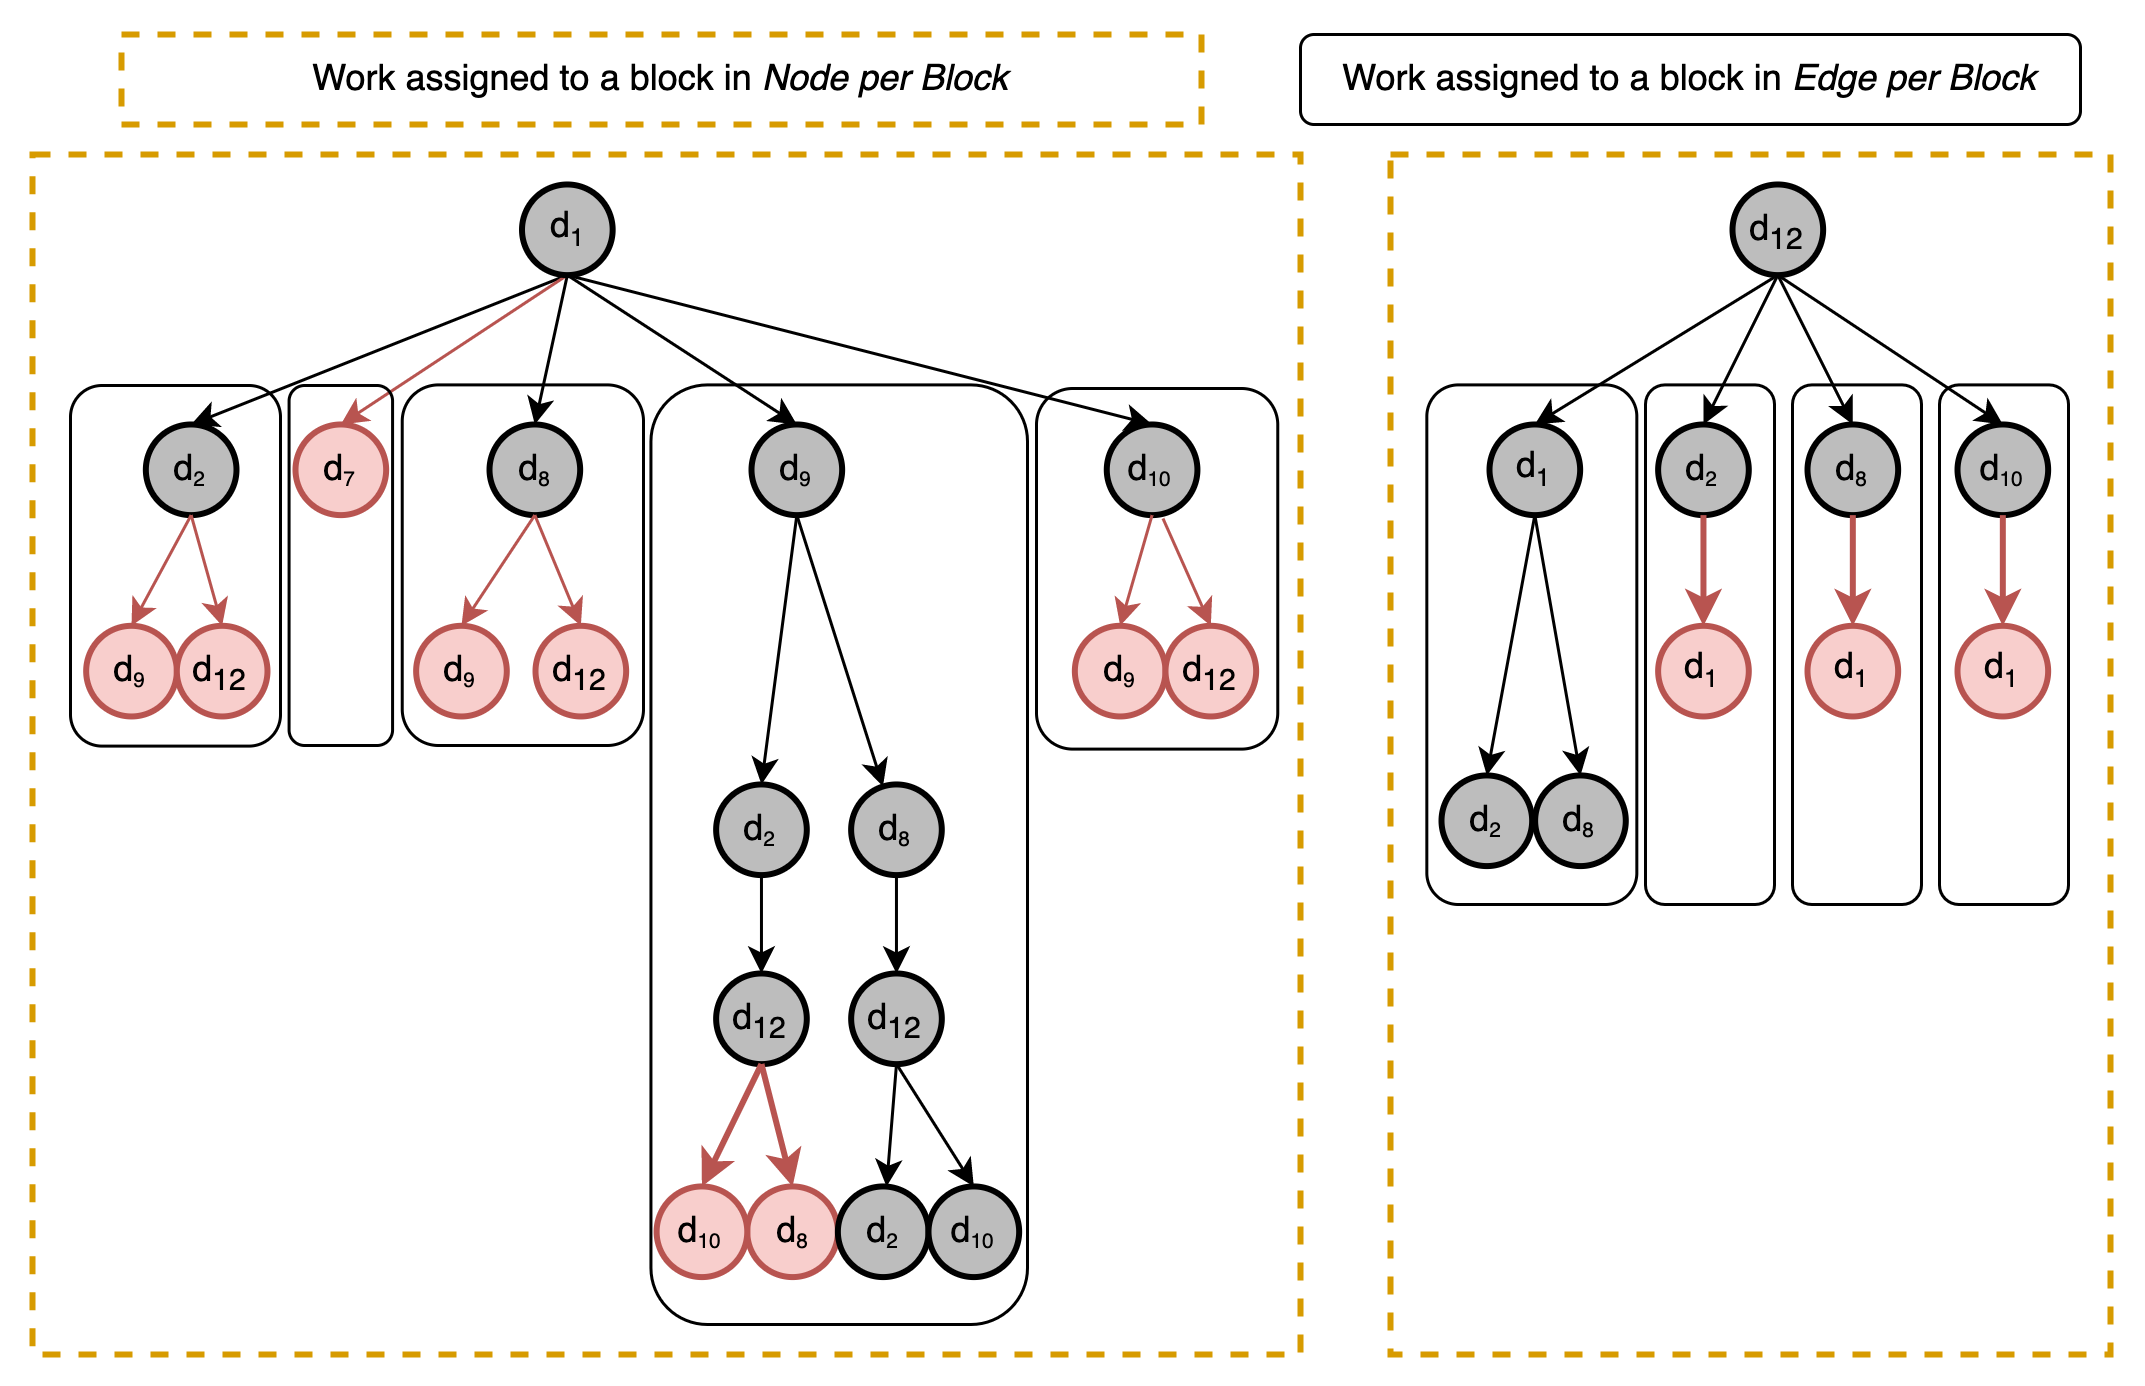
\includegraphics[width=\textwidth]{fig/parallelization-scheme.png}
    \caption{Parallelization Schemes}
    \label{fig:parallelization-schemes}
\end{figure}

Two techniques were implemented to reduce the load imbalance, (1) Task scheduling, and (2) Hybrid Parallelism.
Some runtime insights from the baseline are presented to explain these improvements, these insights also quantify the observations from baseline.
\subsubsection*{Observation 1 - Run time vs Degree}
Figure \ref{fig:runtime-vs-degree} shows the relationship between degree of the root node and runtime as a log-log plot.
It is clear that the run time is exponentially related to the root node degree also there is huge variation in the run time at same degree.
\begin{figure}
    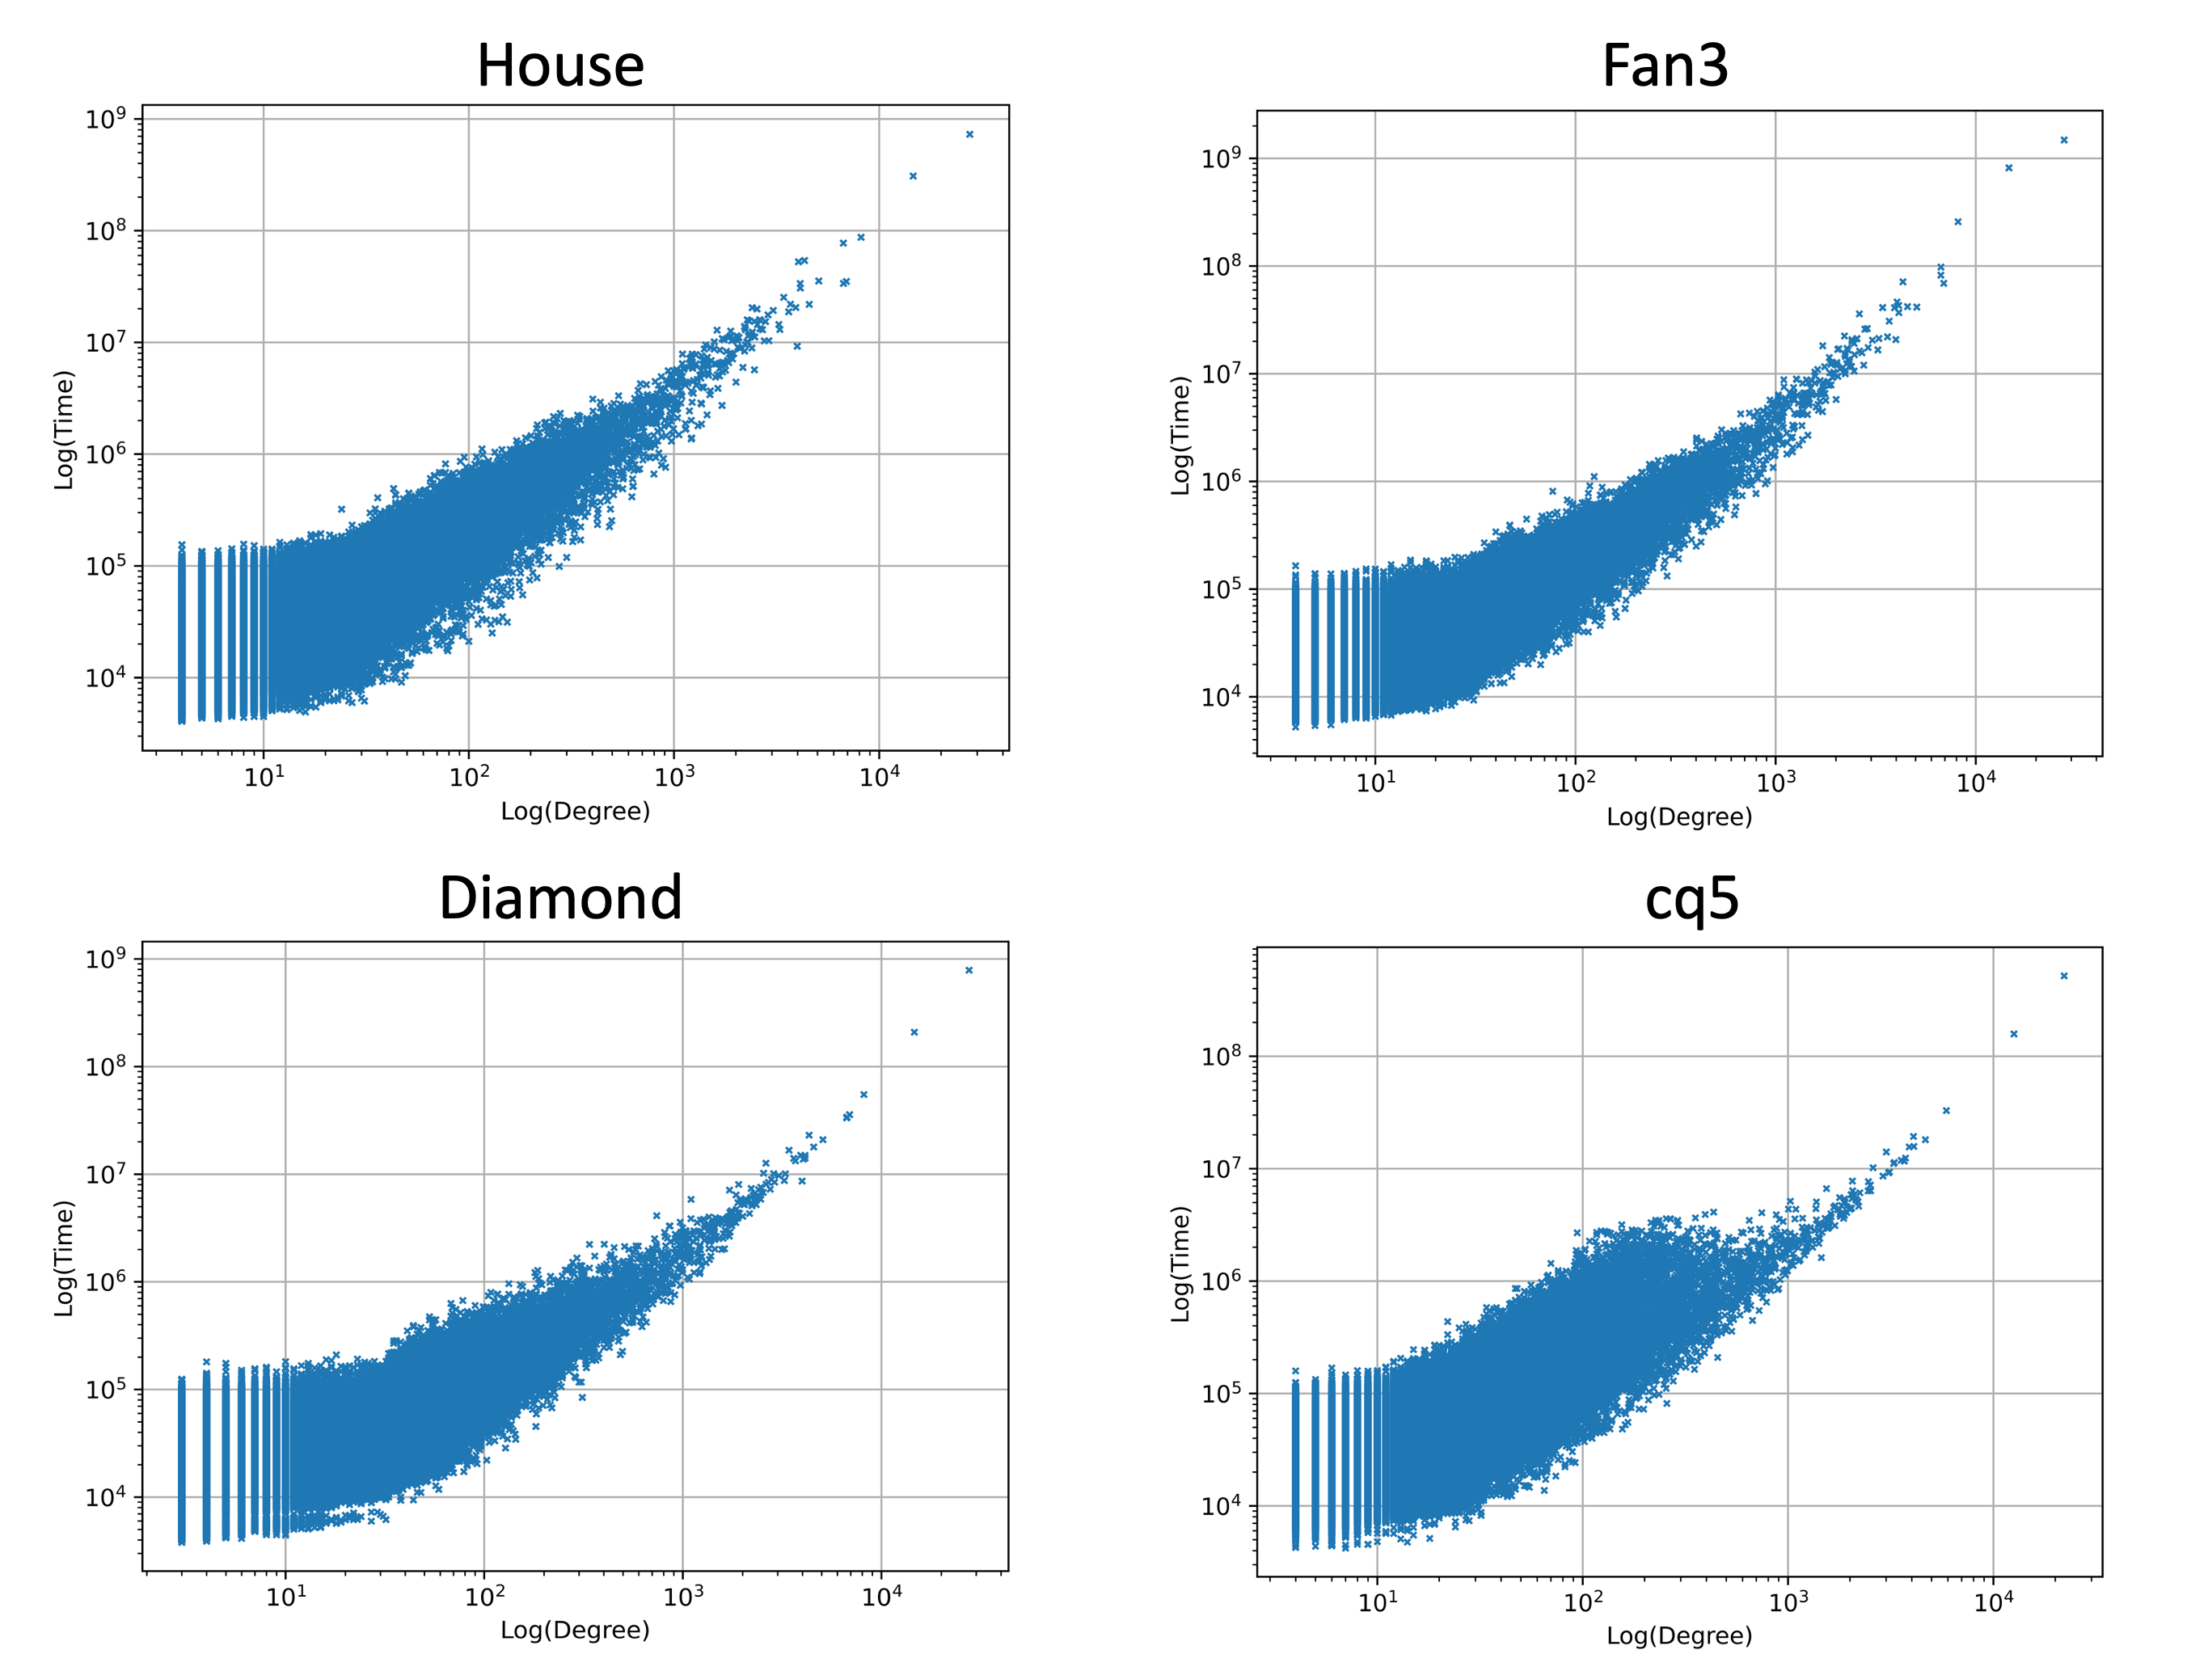
\includegraphics[width=\textwidth]{fig/improvements/time-vs-degree.png}
    \caption{Degree vs Runtime for data graph com-youtube}
    \label{fig:runtime-vs-degree}
\end{figure}

\subsubsection*{Observation 2 - Load balance comparison}
Given the trend between runtime and degree of the root node, the node per block scheme is expected to show a huge load imbalance.
The load balance is supposed to improve for edge per block scheme as it would split the work offered by a high degree root node into several blocks.
Figure \ref{fig:load-balance-baseline} shows the load balance across SMs for various query graphs as standard box plot. This is computed by finding the processing time spent by each SM during the kernel lifetime. These times are then normalized to remove variability due to query graphs. It is clear from the figure that the edge per block parallelization scheme significantly improves load balance.
\begin{figure}
    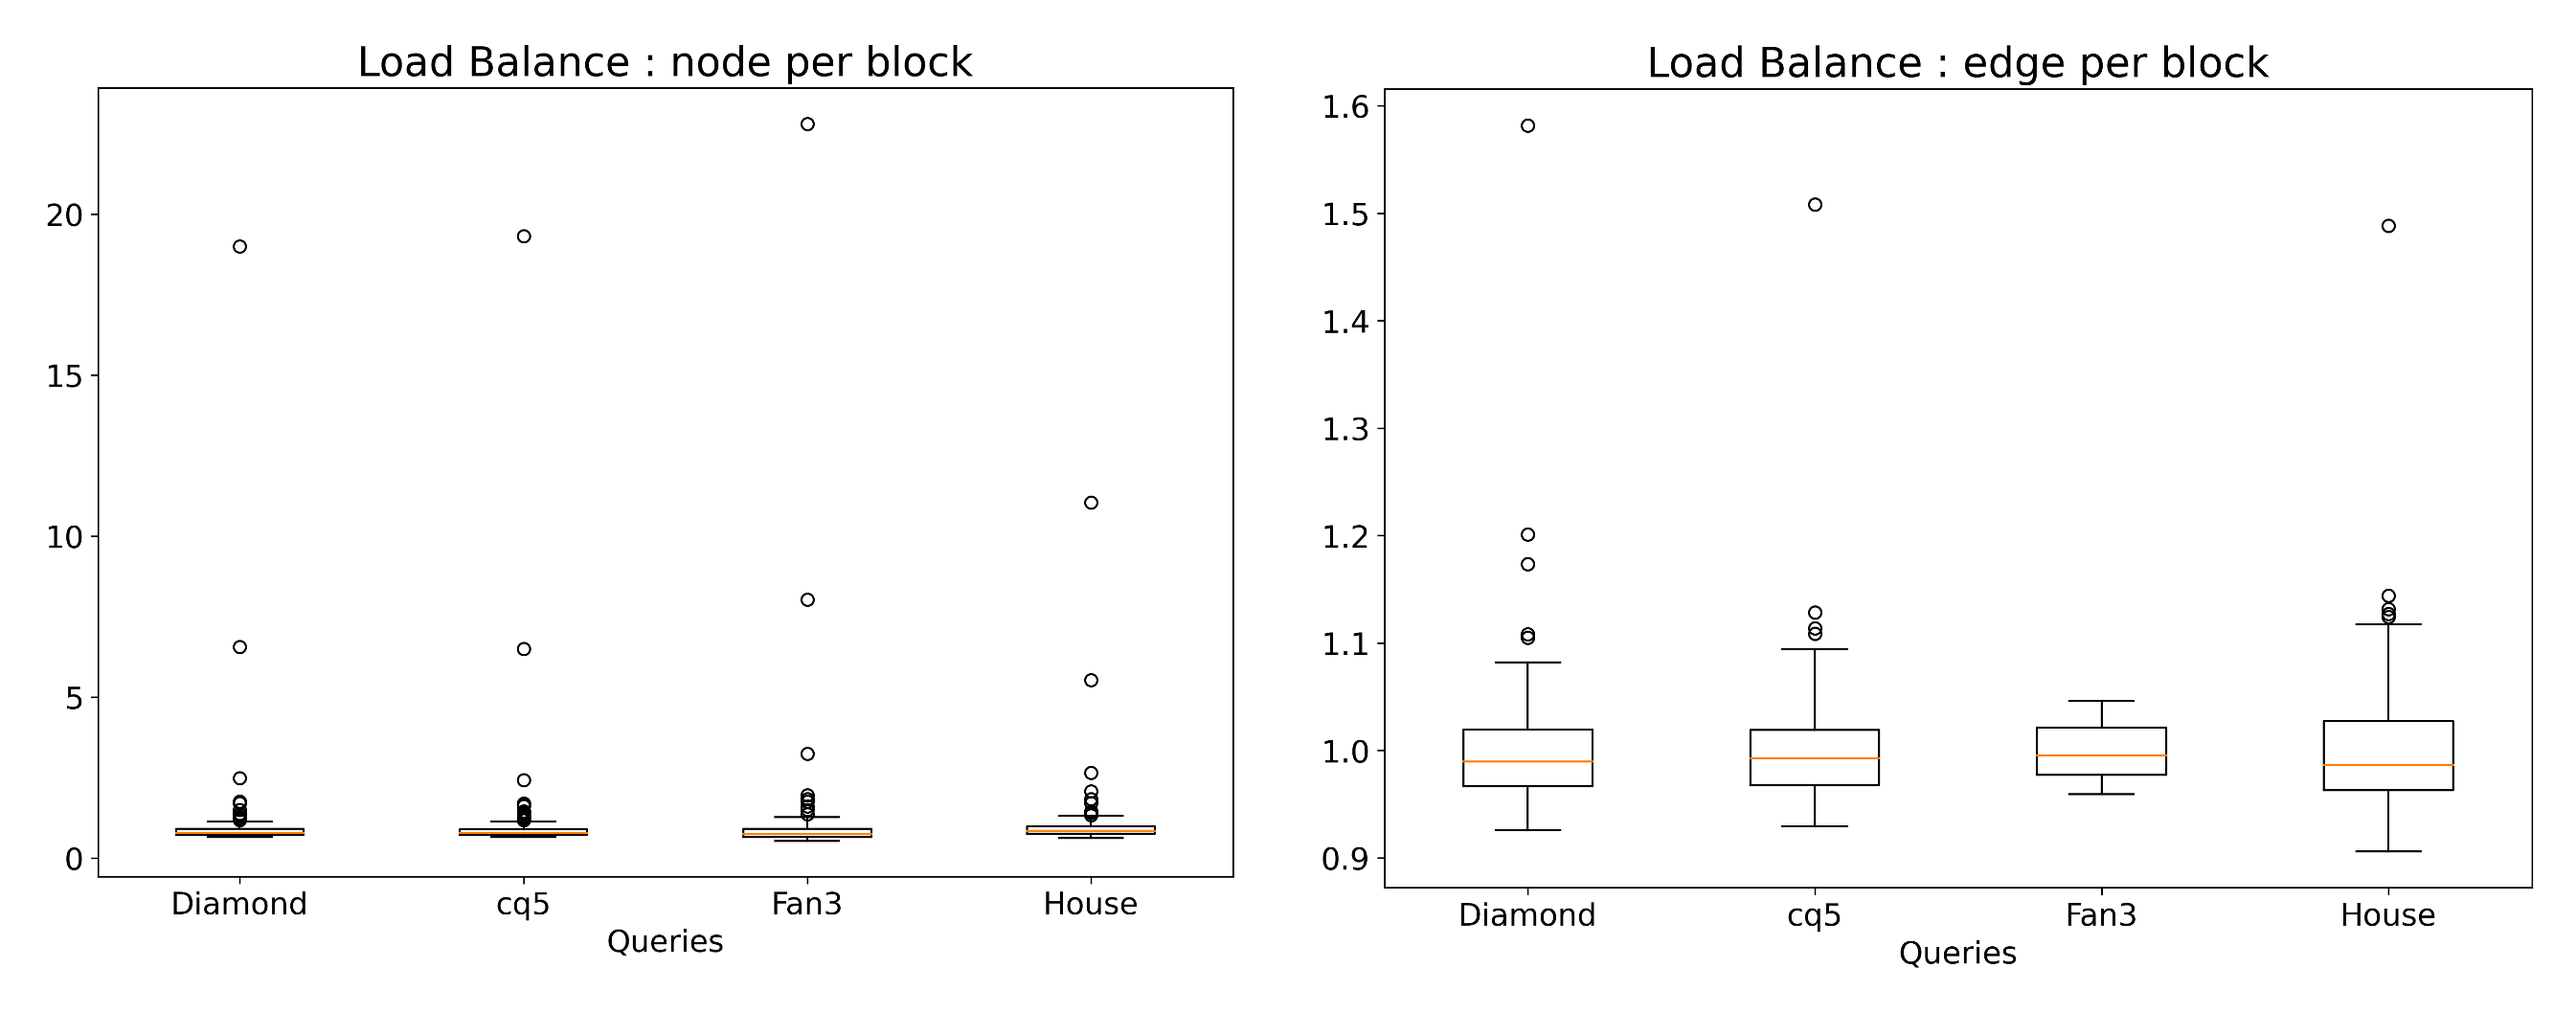
\includegraphics[width=\textwidth]{fig/improvements/yt_lb-baseline_byedge.png}
    \caption{com-youtube load balance with different parallelization schemes}
    \label{fig:load-balance-baseline}
\end{figure}

\subsubsection*{Observation 3 - Load balance for low degree nodes}
Since the trend between degree and runtime is exponential, the subtrees originating from nodes with low degrees will likely have lesser variation in run times.
Figure \ref{fig:load-balance-LD} shows there is negligible load imbalance for low degree nodes.
For these findings, all nodes with degree higher than cutoff were filtered out before kernel launch.
\begin{figure}
    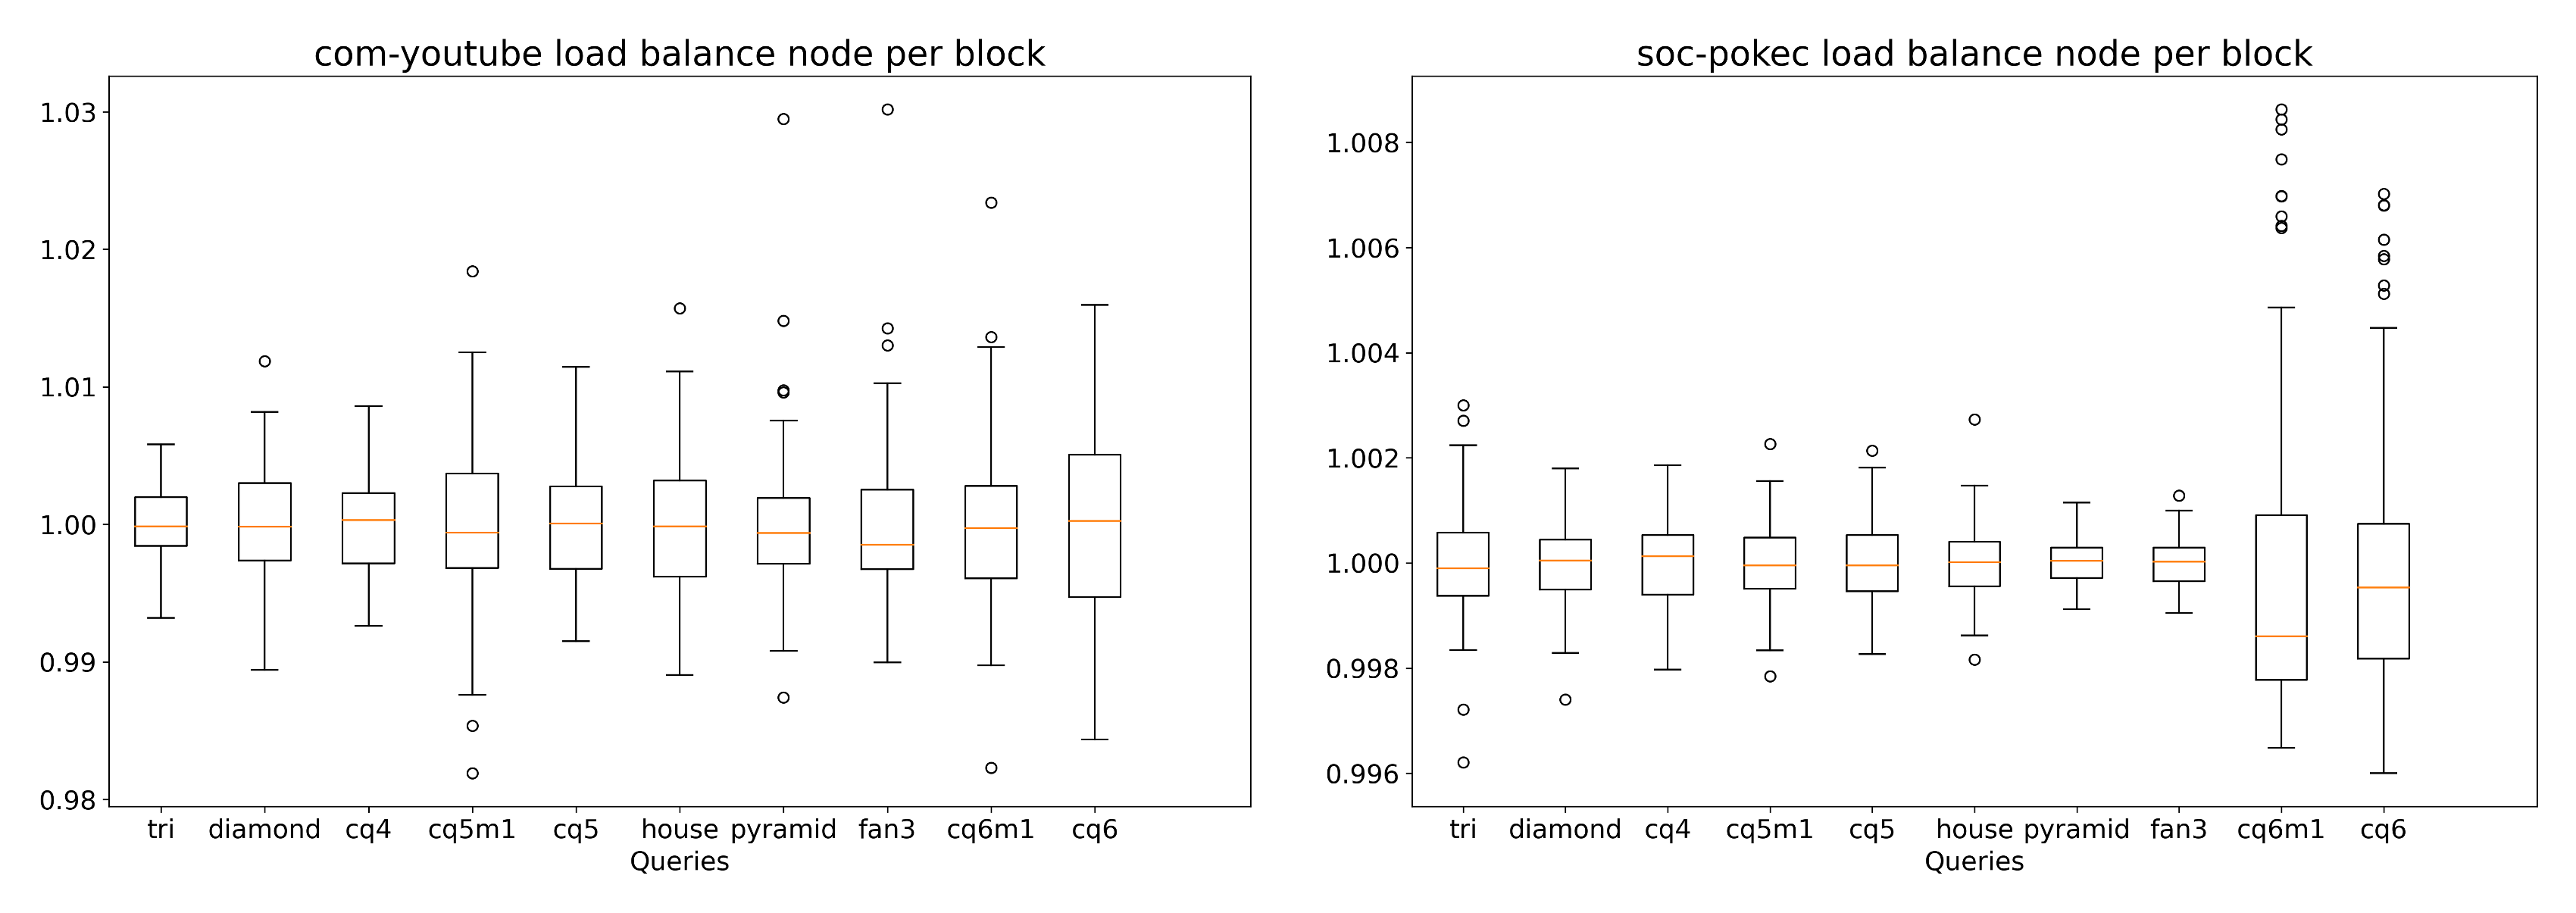
\includegraphics[width=\textwidth]{fig/improvements/load-balance-LD.png}
    \caption{Load balance for nodes with degree $\leq 256$ }
    \label{fig:load-balance-LD}
\end{figure}

The claim from the authors of \cite{PARSEC_VD} was edge per block scheme works better than node per block for queries of size greater than five.
One reason for this claim is implied by the load balance observations above, however, it does not explain the slow performance of the edge per block kernel.
The reason here is strictly based on the implementation. For the edge per block scheme in \cite{PARSEC_VD}, each block induces its subgraph. This causes extra workload hence the edge per block implementation outperforms only for larger query graphs as they exhibit worse load balance.
To remove this redundant work, the kernel is split with different parallelization schemes in each part.
The first kernel ensures non-redundancy while inducing subgraphs by using the node per block scheme.
The second kernel uses these induced subgraphs to perform search tree traversal using the edge per block scheme while ensuring better load balance.

Since the kernels are split, the persistent memory technique used in the baseline \cite{PARSEC_VD} needs to be removed.
To minimize the total number of kernel launches and better resource utilization a runtime query to the device memory is performed and the number of nodes to process at once is found accordingly.

It is clear from Figure \ref{fig:load-balance-LD} that the low degree nodes do not exhibit load imbalance with node per block parallelization. Since, splitting the kernels loses cache benefits and causes launch overheads a cutoff scheme was developed. Nodes with degree less than cutoff would perform subgraph inducing and search tree traversal in node per block fashion while nodes with degree higher than cutoff would perform these operations as mentioned above.
Figure \ref{fig:hybrid-par-speedups} shows the improvement in runtimes for the com-youtube data graph across different queries with cutoff being 2048.

\begin{figure}
    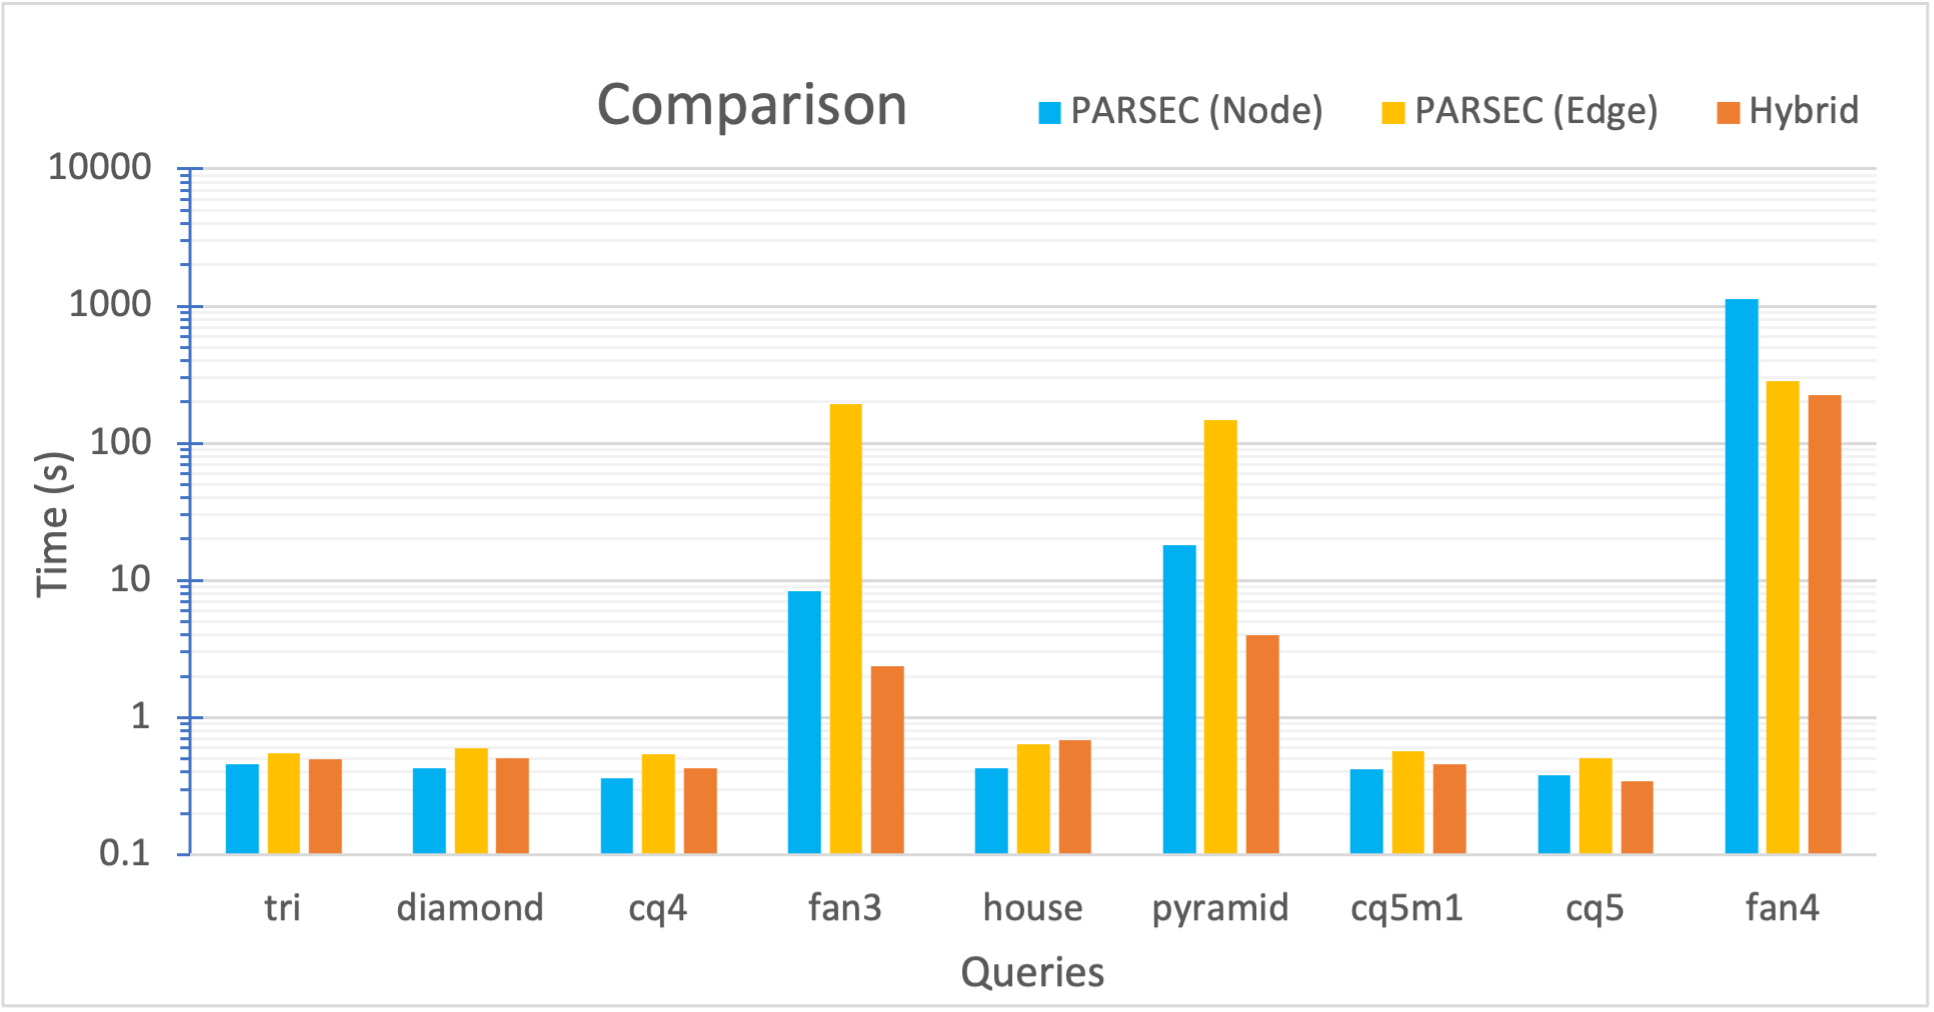
\includegraphics[width=\textwidth]{fig/improvements/Hybrid-parallelism-speedups.png}
    \caption{Run times with Hybrid parallelism for com-youtube with cutoff=2048 }
    \label{fig:hybrid-par-speedups}
\end{figure}

Empirical testing was performed to fix a cutoff value across different queries.
It was found that for dense templates like \textit{cqx} and \textit{cqxm1} cutoff value between $(1024 - 2048)$ is better while for sparse templates like \textit{fans, pyramids,} and \textit{wheels} cutoff value around $768$ achieved best results.
Figure \ref{fig:cutoff-tests} shows the time fraction of runtimes across different cutoffs, time fraction is defined as runtime of an instance divided by average time across all instances (Lower is better for these Figure).
Using these insights the cutoff was decided at runtime based on input query.

\begin{figure}
    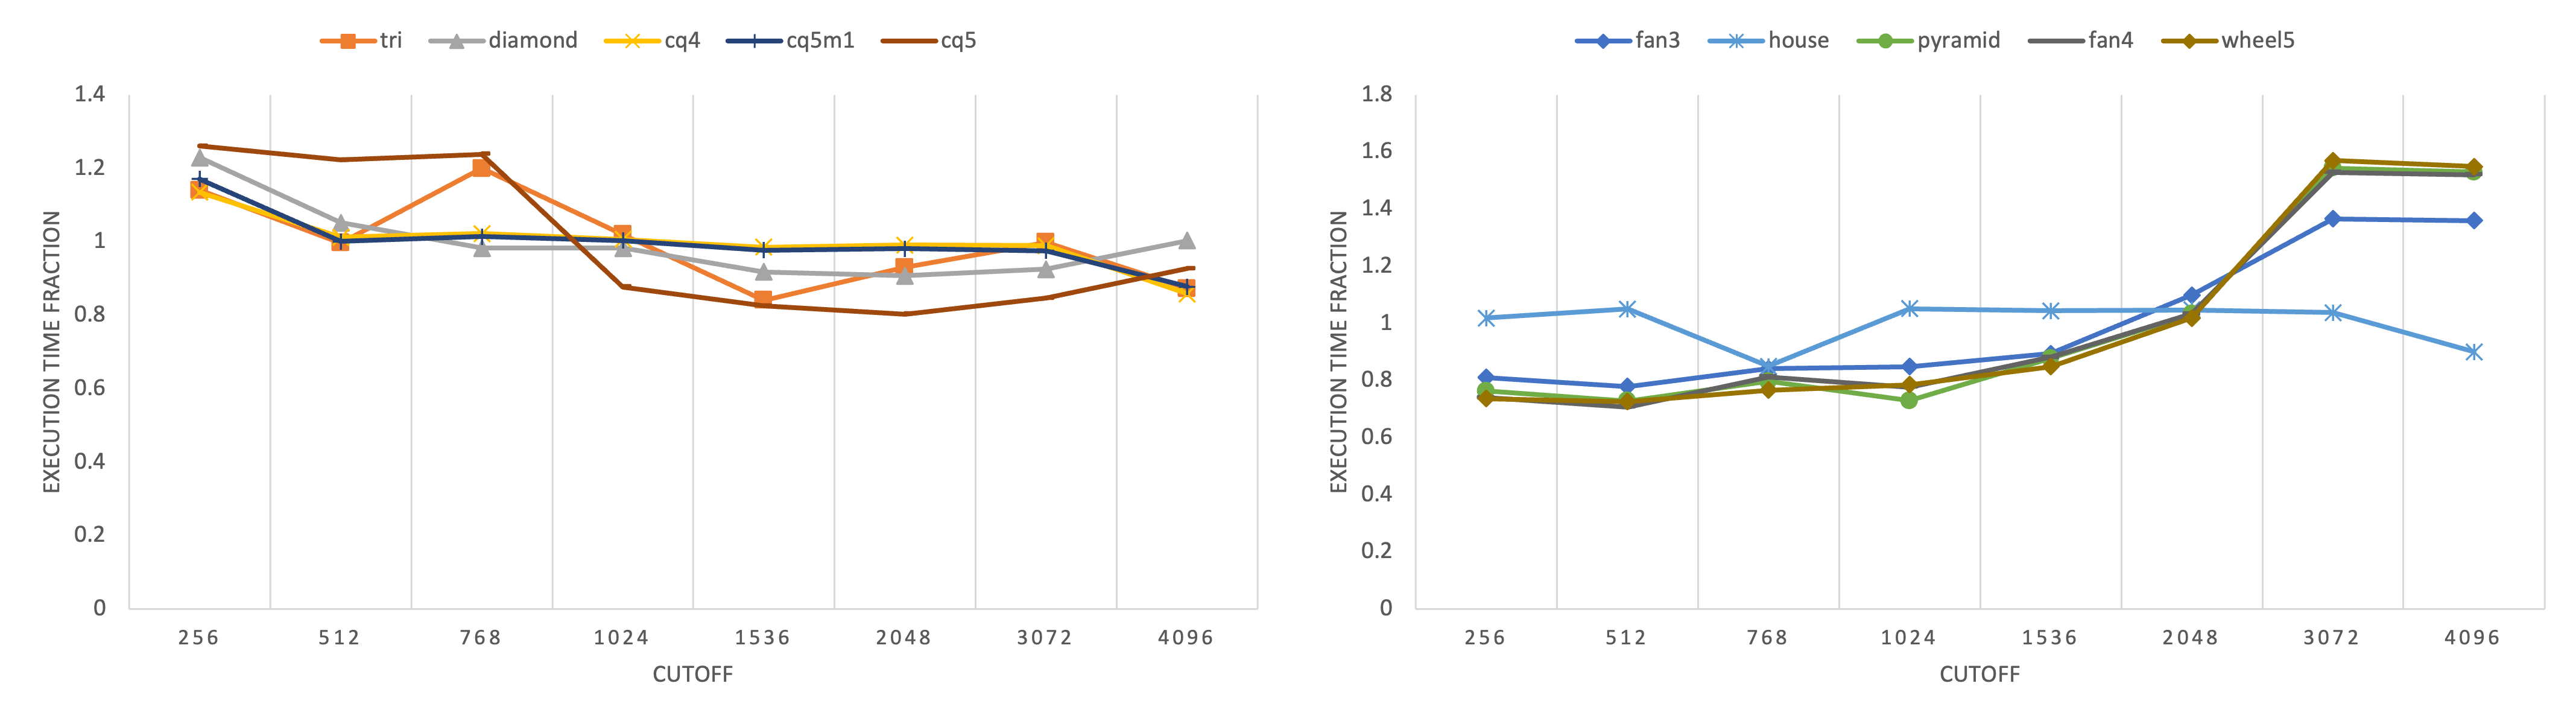
\includegraphics[width=\textwidth]{fig/improvements/cutoff-tests-yt.png}
    \caption{Run time fractions vs cutoff for com-youtube}
    \label{fig:cutoff-tests}
\end{figure}
\chapter{Results}
\label{chap:Results}

\section{Experimental Setup} \label{sec:expt-info}
All results presented in this chapter are generated on a supercomputing hardware cluster with a dual-socket 64-core AMD EPYC 7763 (``Milan") CPU and NVIDIA A100 40GB HBM2 GPU.
The system has 256 GB of DDR4 memory with 1.5 TB swap memory via high-performance-SSD.
The program is compiled with NVCC (CUDA 11.7, driver version 515.48) SM version 80, and GCC 11.2 with the -O3 flag.
For a fair comparison, the baseline is also run on the same hardware platform with equivalent compilation flags.

The data graphs used for experiments are obtained from the Stanford Network Analysis Project (SNAP) \cite{snap}.
Table \ref{tab:graphs} summarizes the properties of these data graphs.

\begin{table}[tbp]
    \centering
    \caption{Data Graphs used for experiments}
    % \resizebox{\textwidth}{!}{%
    \begin{tabular}{@{}crrr@{}}
        \hline
        \multicolumn{1}{c}{\textbf{Graph}} & \multicolumn{1}{c}{$|\textbf{V}|$} & \multicolumn{1}{c}{$|\textbf{E}|$} & \multicolumn{1}{c}{\textbf{Max Degree}} \\ \hline
        as-skitter                         & 1,696,415                          & 11,095,298                         & 35,455                                  \\
        soc-pokec                          & 1,632,804                          & 22,301,964                         & 14,854                                  \\
        % com-dblp                           & 317,080                            & 1,049,866                          & 343                                     \\
        cit-patents                        & 3,774,768                          & 16,518,948                         & 793                                     \\
        % com-lj                             & 3,997,962                          & 34,681,189                         & 14,815                                  \\
        com-orkut                          & 3,072,441                          & 117,185,083                        & 33,313                                  \\
        % com-friendster                     & 65,608,366                         & 1,806,067,135                      & 5,214                                   \\
        com-youtube                        & 1,134,891                          & 5,975,248                          & 28,754                                  \\
        \hline
    \end{tabular}%
    % }
    \label{tab:graphs}
\end{table}

We use the common query graphs with central nodes that are generally used in subgraph enumeration literature.
Figure \ref{fig:queries} shows the query graphs used for experiments, these queries are adapted from \cite{PARSEC_VD}.
\textit{Clique} is a fully connected graph.
As a notation in Figures and Tables, we use cqx for \textit{clique} of size x and cqxm1 for size x \textit{clique} with one edge missing. Note, removing exactly one edge from a \textit{clique} gives a unique query due to symmetry.
\begin{figure}[t]
    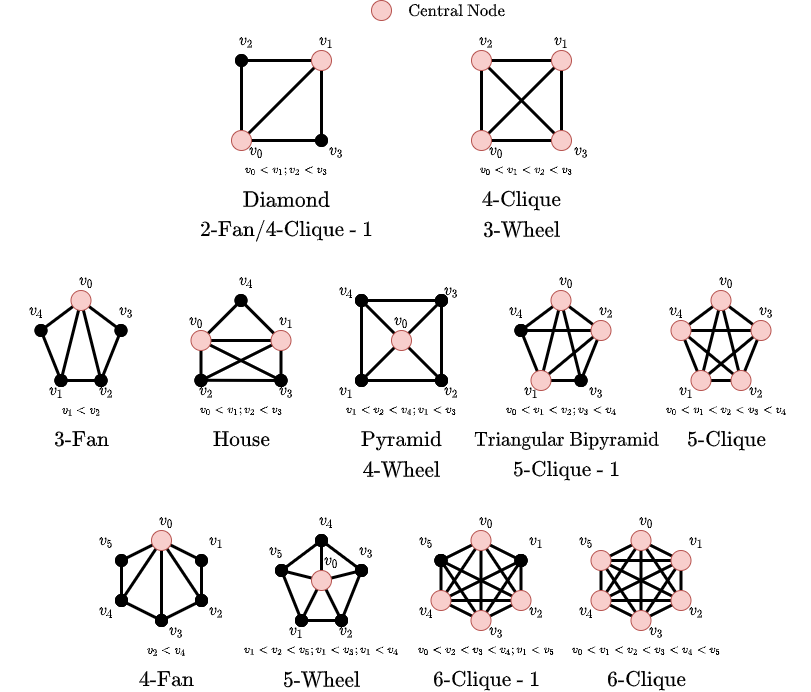
\includegraphics[width=\textwidth]{fig/improvements/Templates.png}
    \source{PARSEC \cite{PARSEC_VD}}
    \caption{Query Graphs used for experiments}
    \label{fig:queries}
\end{figure}

\section{Performance Criteria}
The performance is evaluated in terms of total processing time which includes query preprocessing, data graph preprocessing, and search tree traversal times.
We use the following rules for reporting run times:\
\begin{enumerate}
    \item For instances with total run times less than 1 second, the program is executed 5 times and average times are reported.
    \item Time taken for compilation, reading data graphs, and printing all enumerations is not considered for baseline and our implementation.
    \item The baseline presents 2 parallelization schemes with the comment that the edge per block scheme works better than node per block for templates of size greater than five. This observation is used for fixing one parallelization scheme for comparison.
    \item Instances that take more than 12,000 seconds ($\sim 3.3$ hours) are terminated, and their times are not reported. The corresponding speedup values are reported as blank in all tables.
\end{enumerate}


\section{Final Results and Analysis}



\begin{table}
    \centering
    \caption{Speedups across all queries and data graphs}
    \resizebox{\textwidth}{!}{%
        \begin{tabular}{c|ccccc|c}
            \textbf{Queries}  & \textbf{soc-pokec} & \textbf{com-youtube} & \textbf{cit-patents} & \textbf{com-orkut} & \textbf{as-skitter} & \textbf{Geo Mean} \\
            \hline
            Tri               & 1.49               & 2.11                 & 1.00                 & 0.73               & 1.95                & 1.35              \\
            Diamond           & 1.44               & 2.31                 & 1.00                 & 0.92               & 2.08                & 1.45              \\
            cq4               & 1.47               & 2.51                 & 1.03                 & 0.76               & 1.85                & 1.40              \\
            cq5m1             & 1.41               & 2.62                 & 1.08                 & 1.23               & 1.76                & 1.54              \\
            cq5               & 1.46               & 3.04                 & 1.07                 & 1.13               & 1.83                & 1.58              \\
            house             & 1.41               & 2.27                 & 1.08                 & 1.36               & 3.45                & 1.75              \\
            pyramid           & 1.50               & 14.65                & 1.15                 & 4.5                & 9.75                & 4.06              \\
            fan3              & 1.50               & 9.38                 & 1.26                 & 3.59               & 5.89                & 3.27              \\
            cq6m1             & 4.19               & 3.09                 & 5.47                 & 2.41               & 1.44                & 3.01              \\
            fan4              & 3.41               & 5.82                 & 2.62                 & --                 & --                  & 3.73              \\
            wheel5            & 3.39               & 5.93                 & 2.10                 & --                 & --                  & 3.48              \\
            cq6               & 5.68               & 3.65                 & 5.76                 & 4.48               & 2.01                & 4.04              \\
            cq7m1             & 3.19               & 3.14                 & 5.11                 & 1.47               & 1.11                & 2.42              \\
            cq7               & 4.43               & 3.96                 & 5.45                 & 2.01               & 1.32                & 3.03              \\
            cq8m1             & 2.32               & 2.88                 & 3.25                 & 1.32               & --                  & 2.31              \\
            cq8               & 3.55               & 4.06                 & 5.15                 & 1.58               & --                  & 3.29              \\
            cq9m1             & 1.44               & 2.93                 & 2.65                 & 1.32               & --                  & 1.96              \\
            cq9               & 2.32               & 4.06                 & 3.67                 & 1.52               & --                  & 2.69              \\
            \hline
            \textbf{Geo Mean} & 2.25               & 3.74                 & 2.20                 & 1.61               & 2.29                & 2.33
        \end{tabular}%
    }
    \label{tab:speedups}
\end{table}

\begin{figure}
    \centering
    \subfigure[Data Graph: soc-pokec]{
        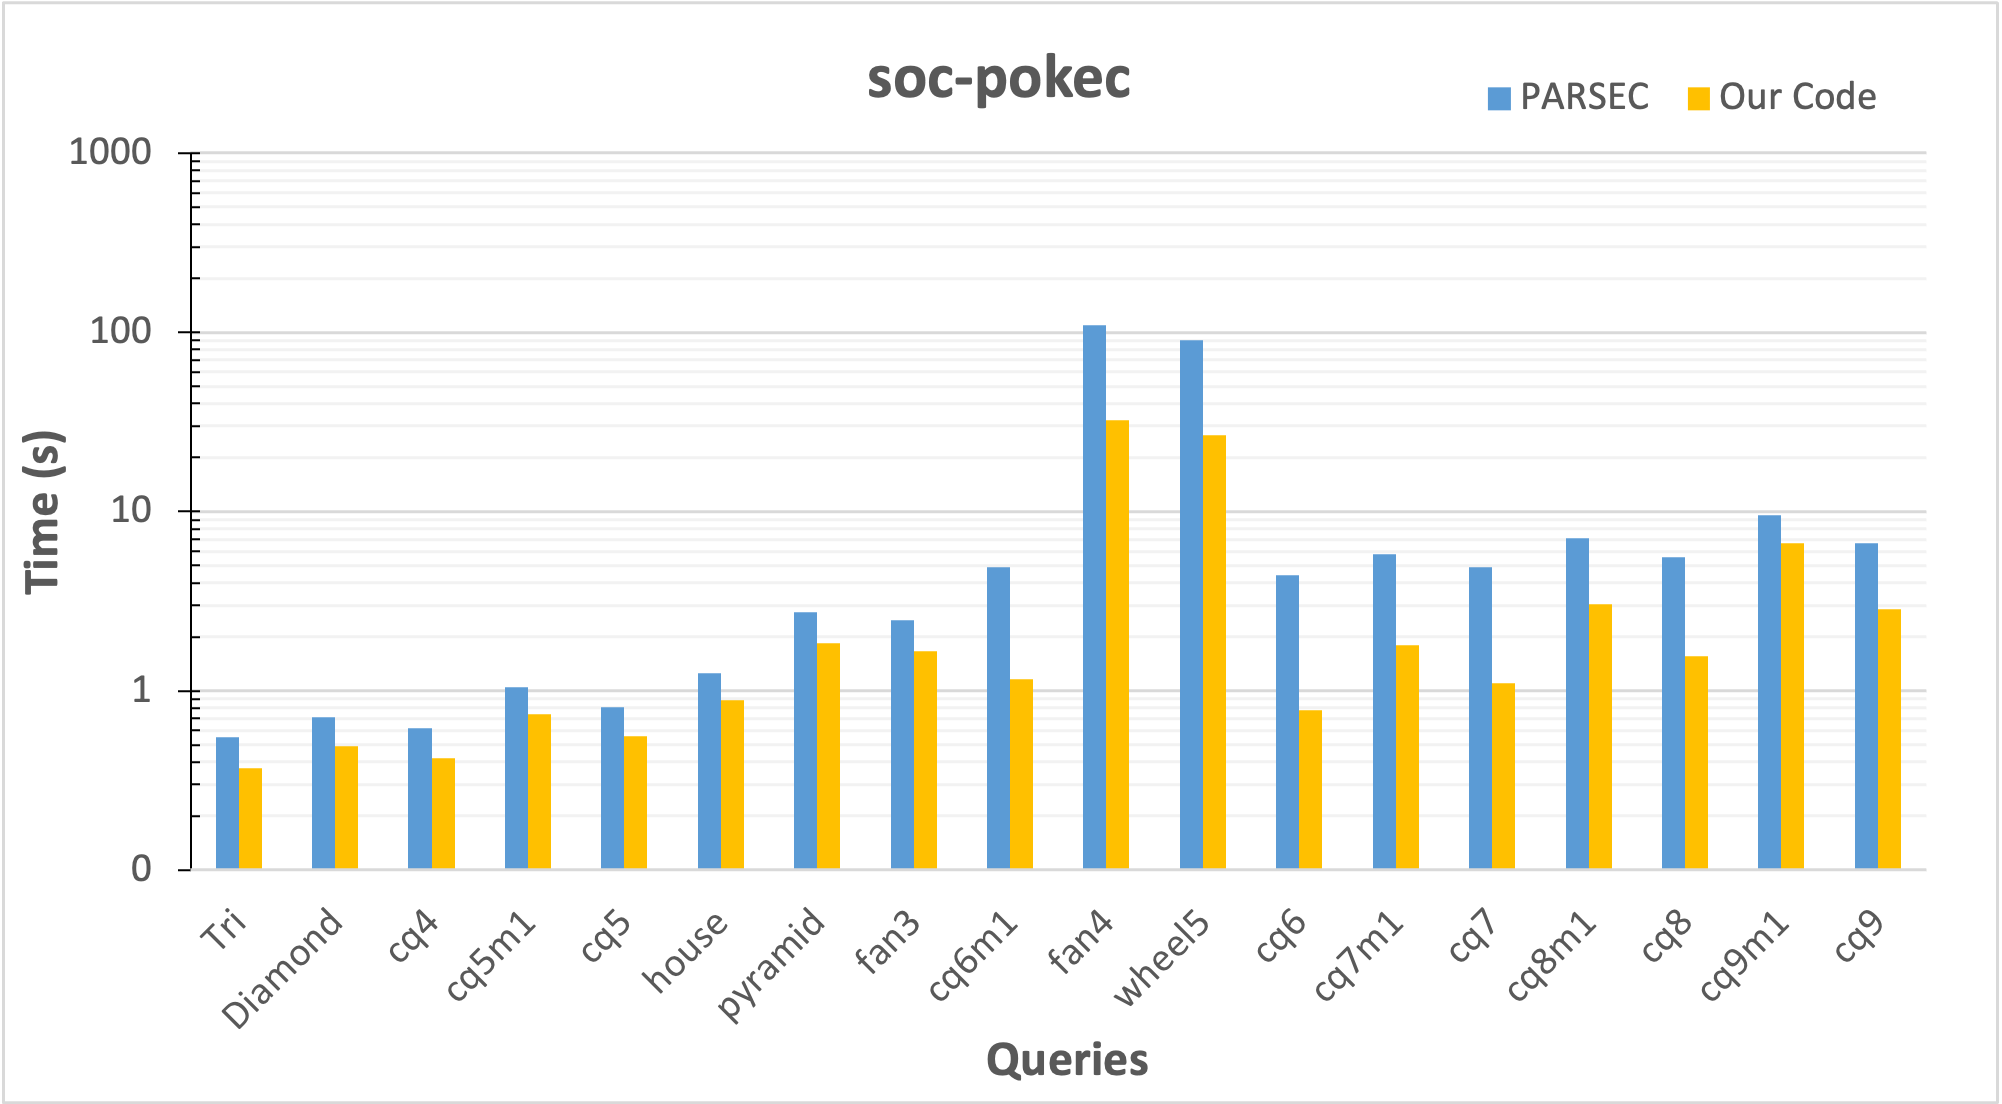
\includegraphics[width=\linewidth]{fig/Results/soc-pokec_times.png}
    }
    \subfigure[Data Graph: com-youtube]{
        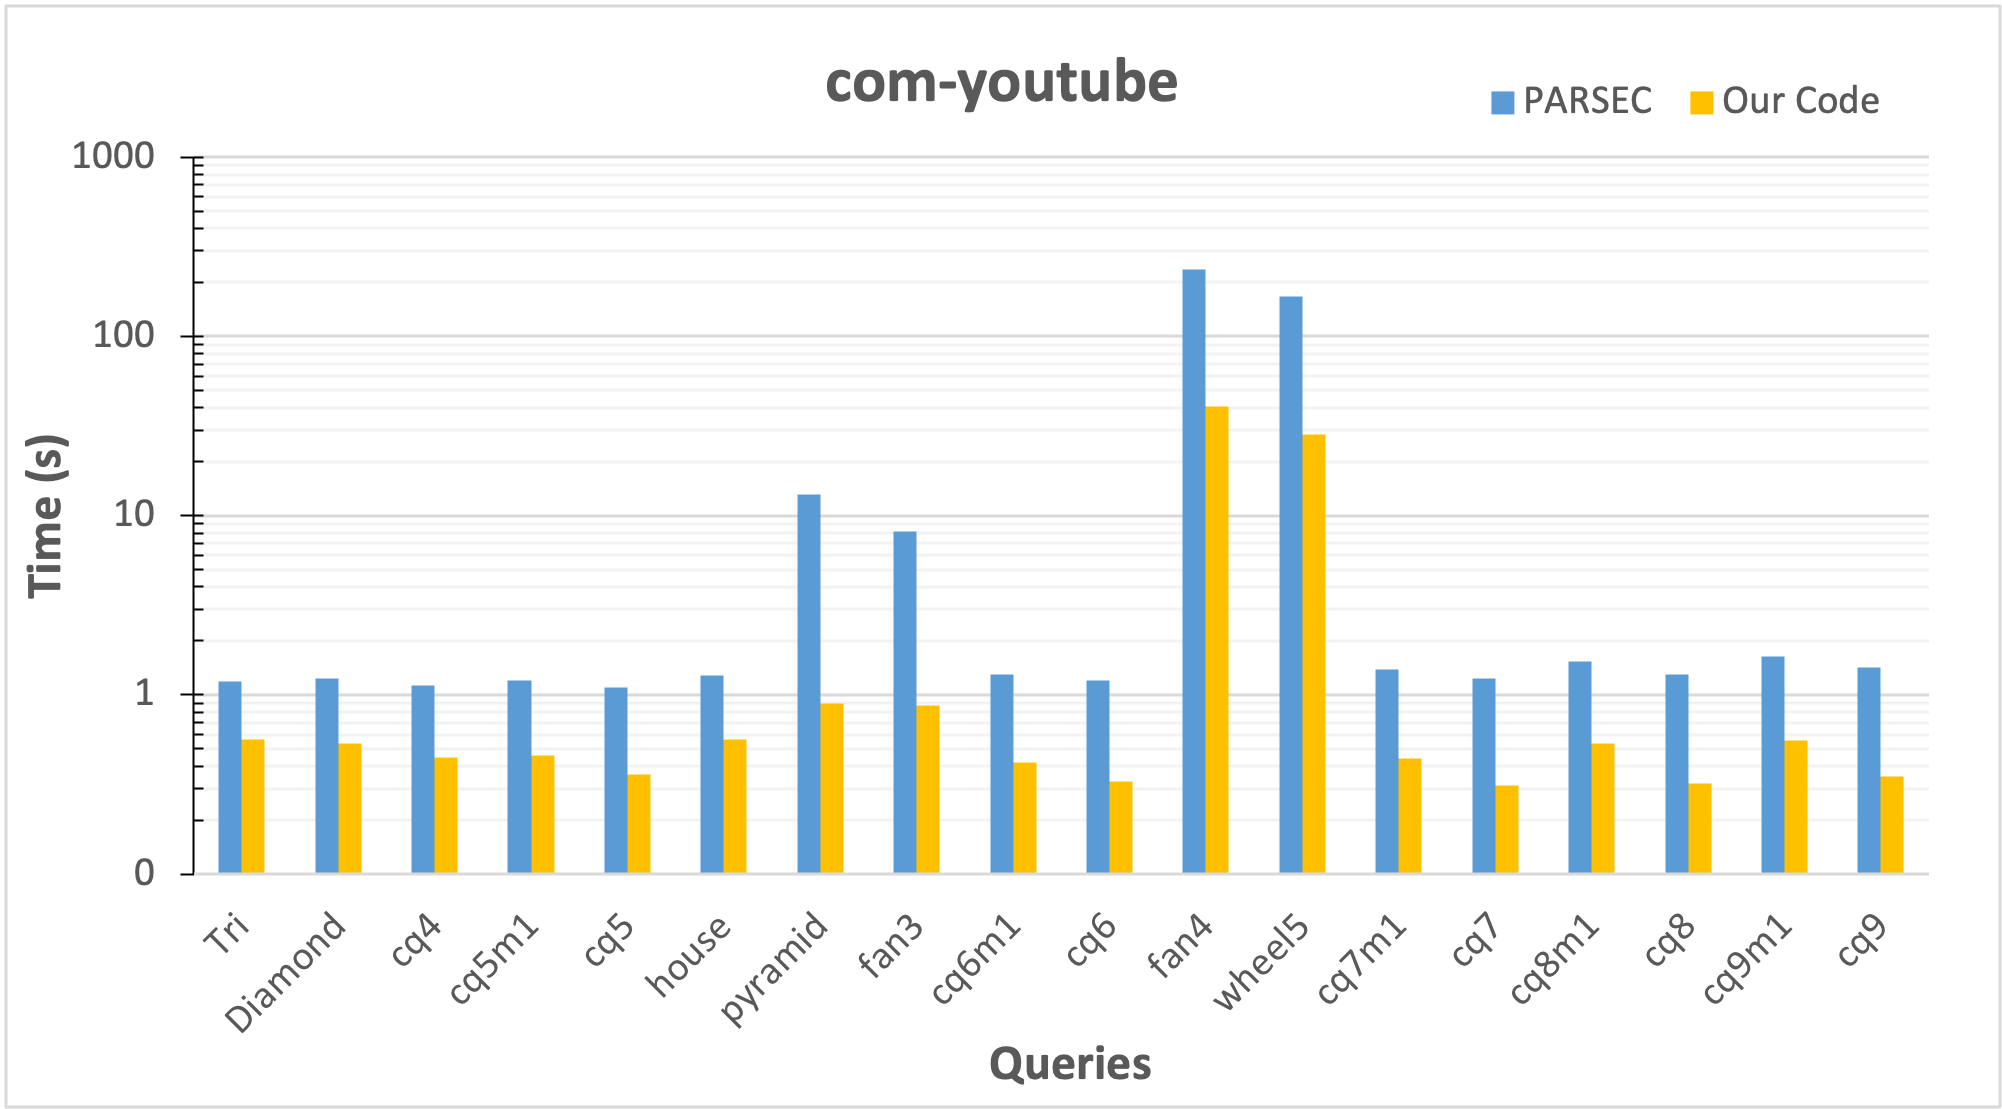
\includegraphics[width=\linewidth]{fig/Results/com-youtube_times.png}
    }
    \caption{Execution times and speedups compared to PARSEC \cite{PARSEC_VD}}
    \label{fig:gpu_comp}
\end{figure}
\begin{figure}\ContinuedFloat
    \centering
    \setcounter{subfigure}{2}
    \subfigure[Data Graph: cit-patents]{
        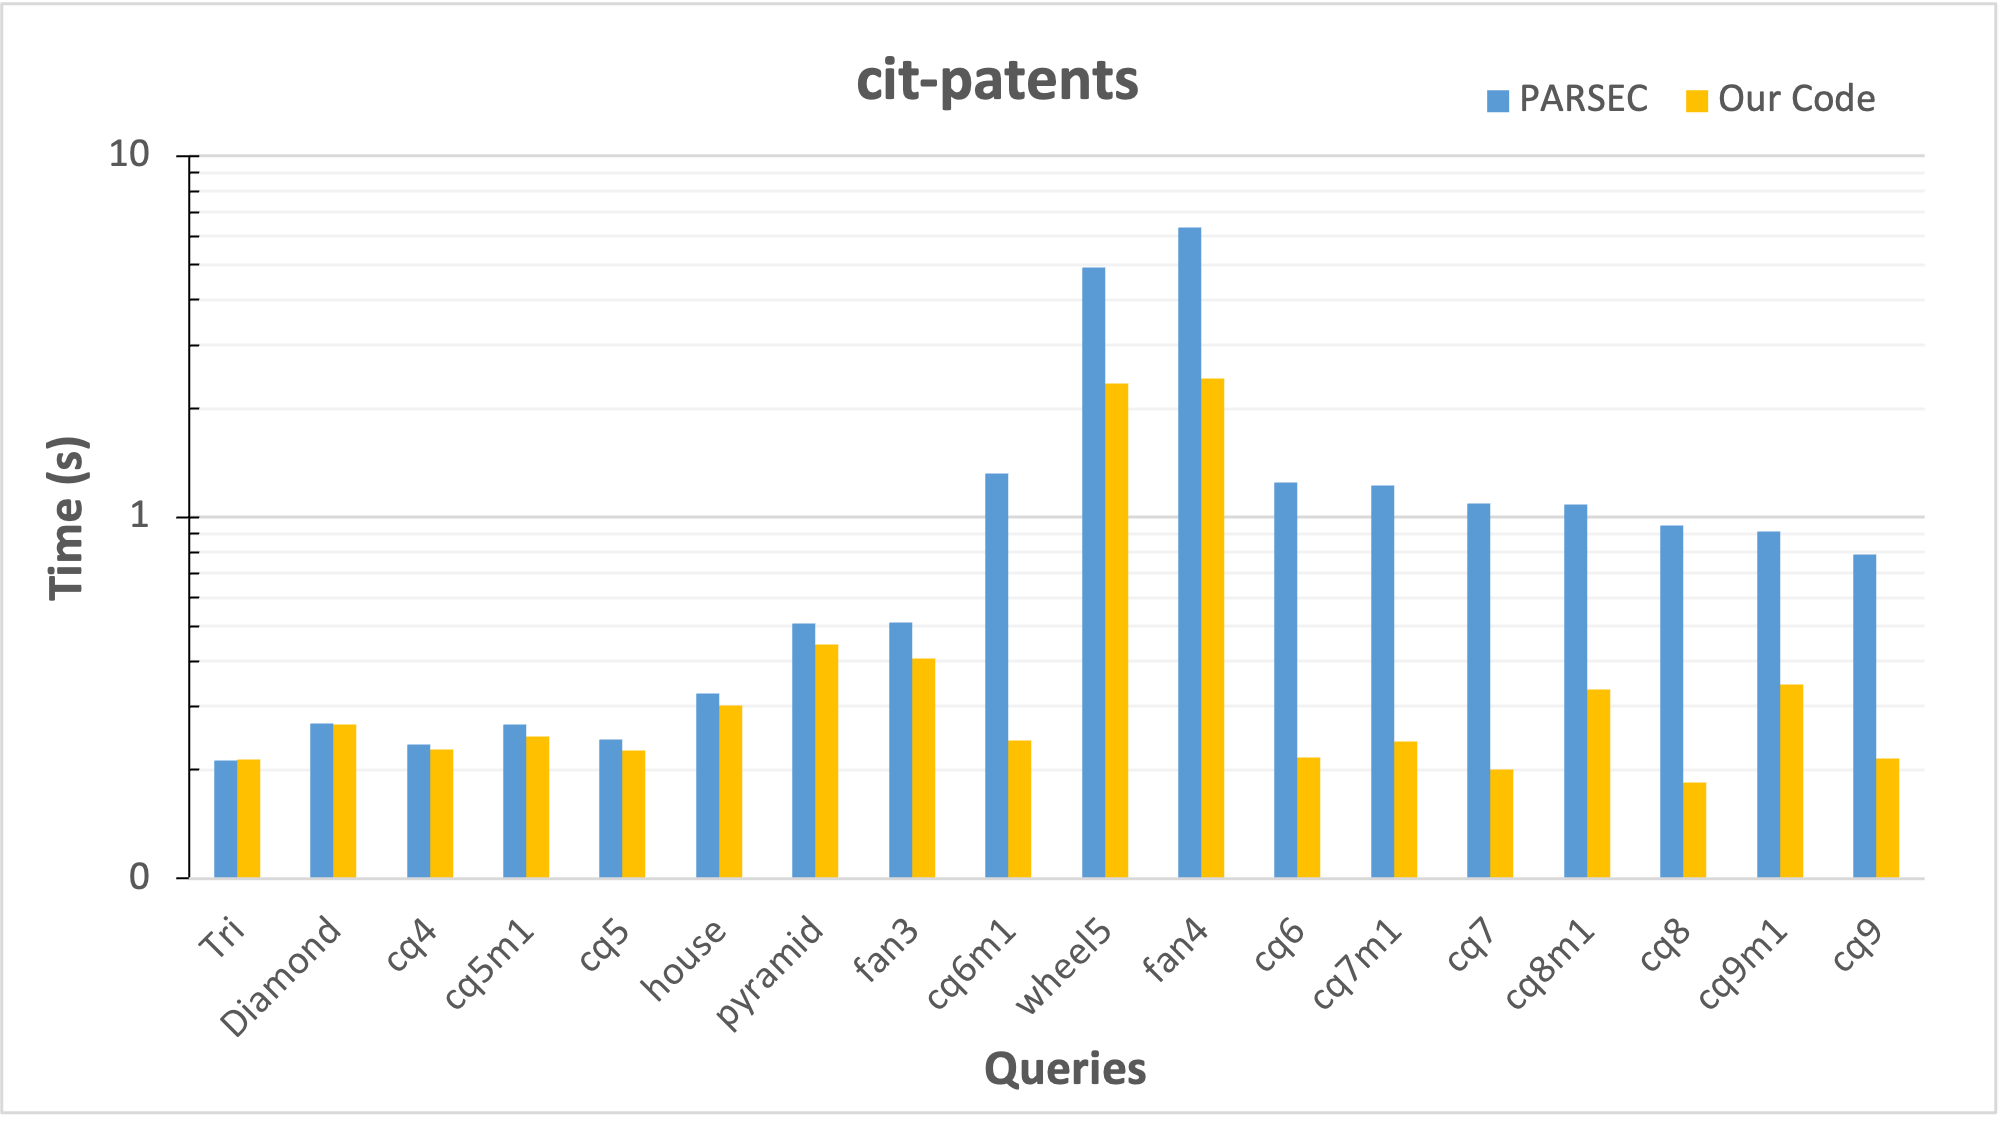
\includegraphics[width=\linewidth]{fig/Results/cit-patents_times.png}
    }
    \subfigure[Data Graph: com-orkut]{
        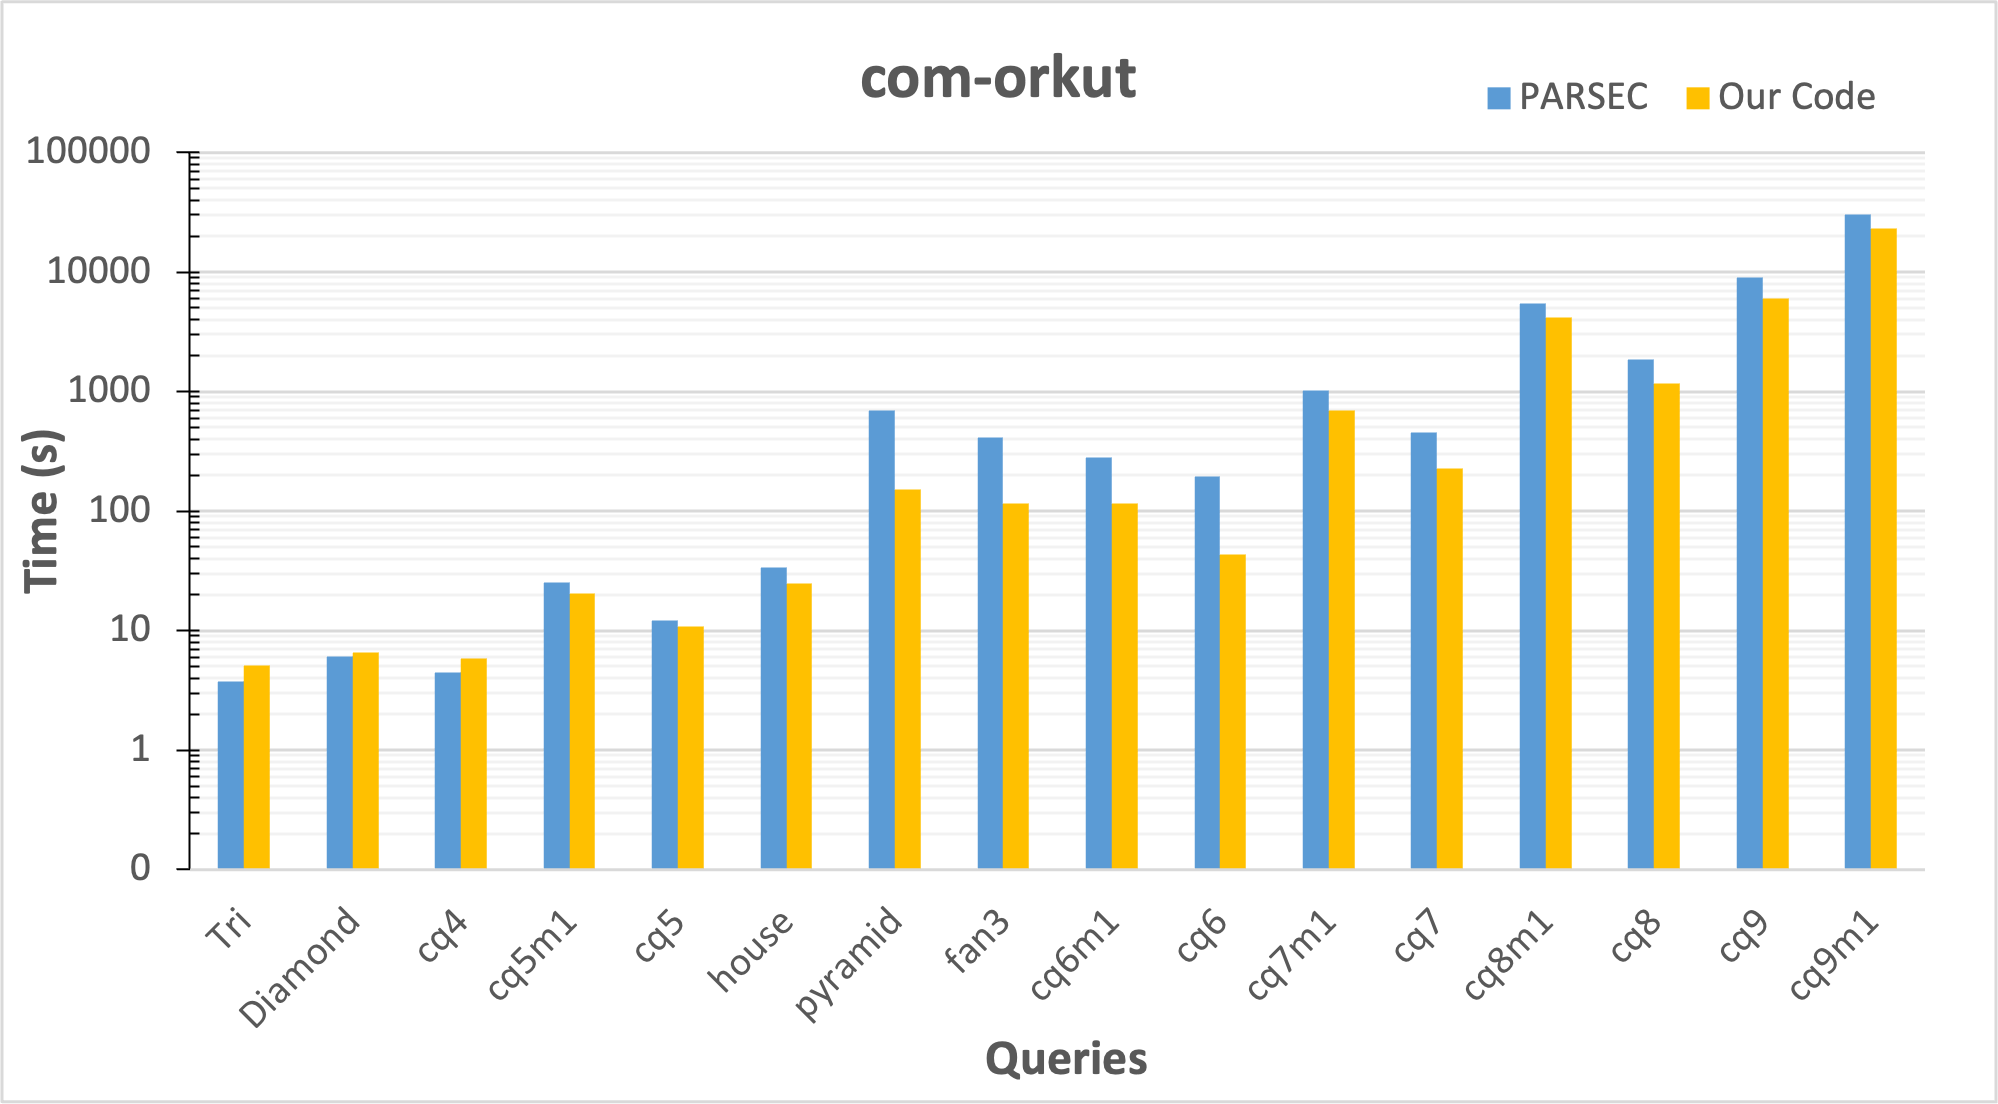
\includegraphics[width=\linewidth]{fig/Results/com-orkut_times.png}
    }
    \caption{Execution times and speedups compared to PARSEC \cite{PARSEC_VD}}
\end{figure}
\begin{figure}\ContinuedFloat
    \centering
    \setcounter{subfigure}{4}
    \subfigure[Data Graph: as-skitter]{
        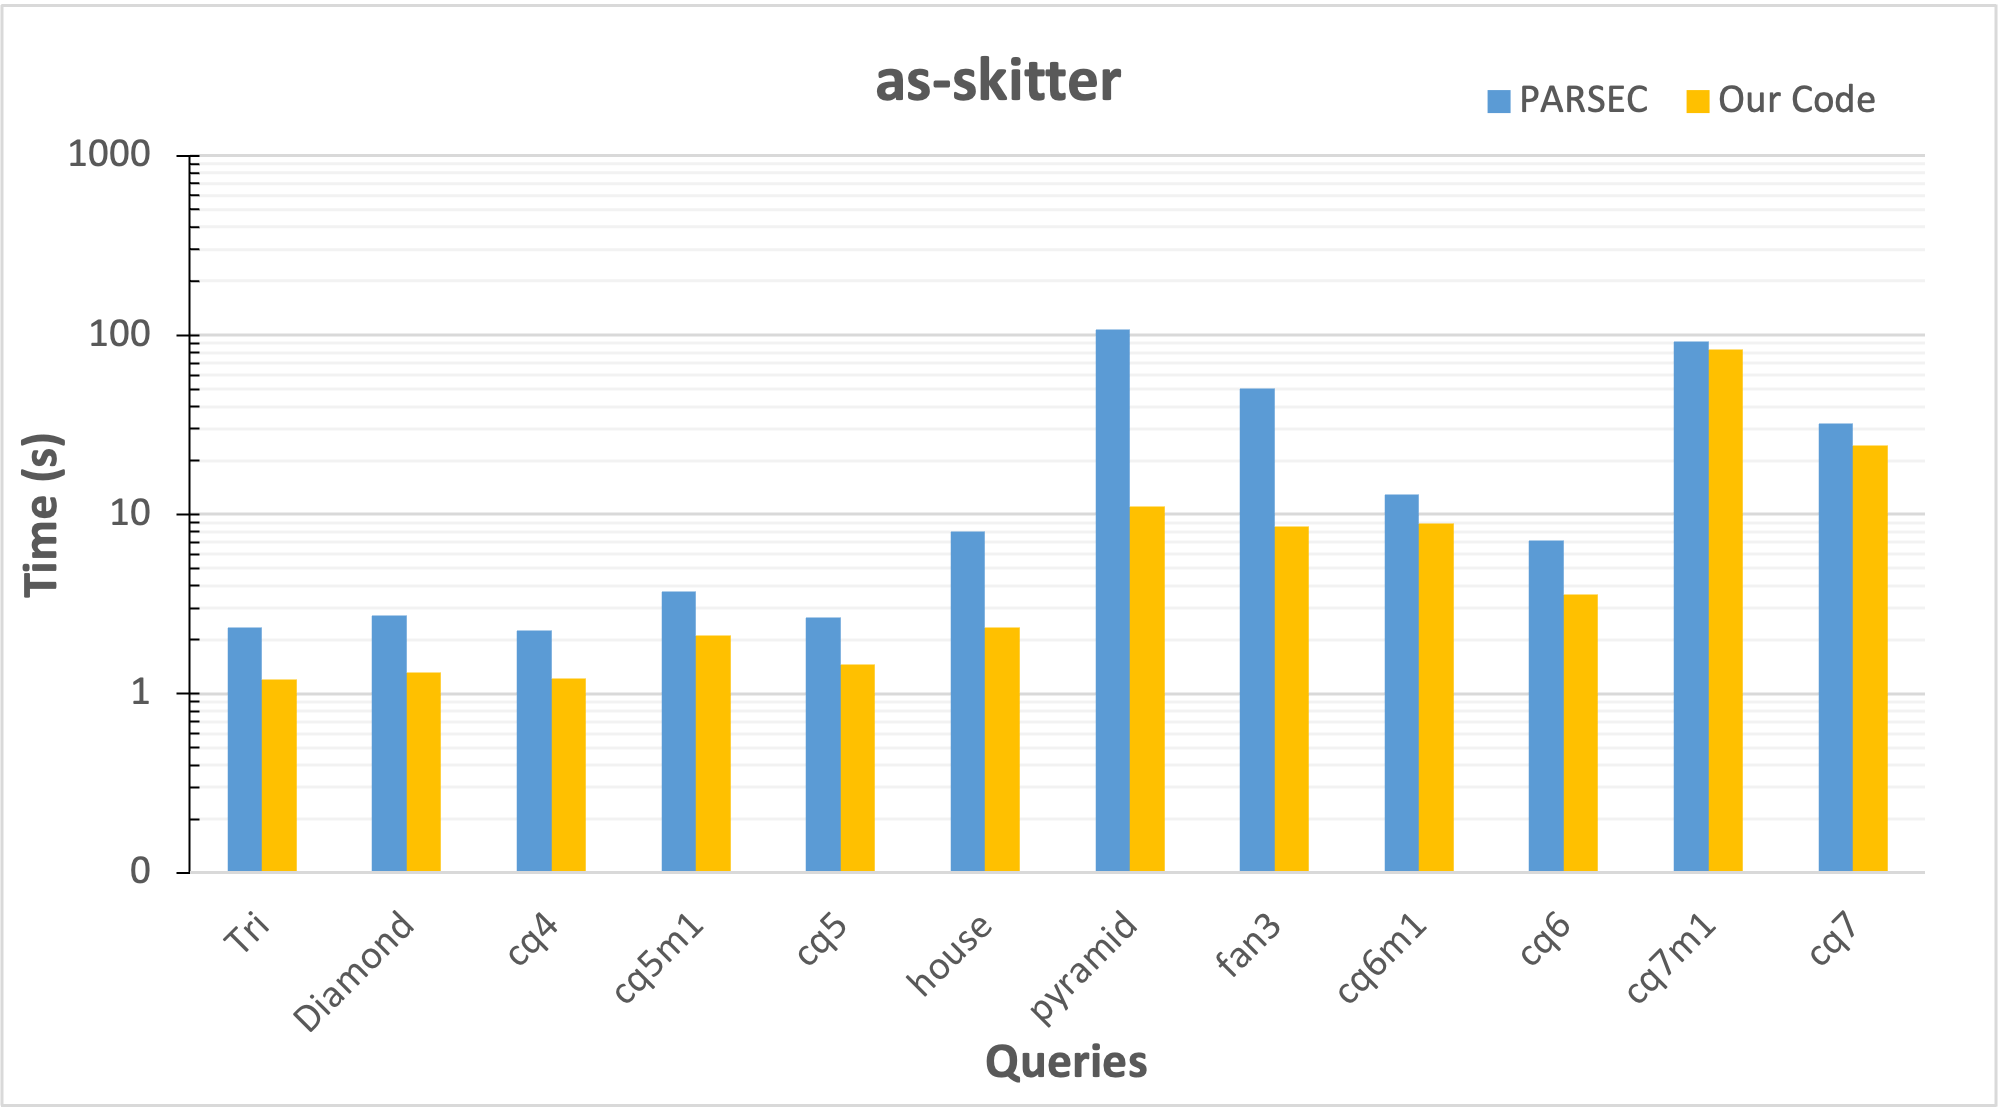
\includegraphics[width=\linewidth]{fig/Results/as-skitter_times.png}
    }
    \caption{Execution times and speedups compared to PARSEC \cite{PARSEC_VD}}
\end{figure}

% \begin{table}[]
%     \centering
%     \resizebox{\textwidth}{!}{%
%         \begin{tabular}{c|cccccccccccccccccc|c}\hline
%             \multirow{2}{*}{data graphs}                                                     & \multicolumn{18}{|c|}{} & \multirow{2}{*}{\textbf{\begin{tabular}[c]{@{}c@{}}Geo-mean\\ (across Queries)\end{tabular}}}                                                                                                                                                 \\
%                                                                                              & Tri                     & Diamond                                                                                       & cq4  & cq5m1 & cq5  & house & pyramid & fan3 & cq6m1 & fan4    & wheel5  & cq6  & cq7m1 & cq7  & cq8m1   & cq8     & cq9m1   & cq9     &      \\
%             \hline
%             \textbf{soc-pokec}                                                               & 1.49                    & 1.44                                                                                          & 1.47 & 1.41  & 1.46 & 1.41  & 1.50    & 1.50 & 4.19  & 3.41    & 3.39    & 5.68 & 3.19  & 4.43 & 2.32    & 3.55    & 1.44    & 2.32    & 2.25 \\
%             \textbf{com-youtube}                                                             & 2.11                    & 2.31                                                                                          & 2.51 & 2.62  & 3.04 & 2.27  & 14.65   & 9.38 & 3.09  & 5.82    & 5.93    & 3.65 & 3.14  & 3.96 & 2.88    & 4.06    & 2.93    & 4.06    & 3.74 \\
%             \textbf{cit-patents}                                                             & 1.00                    & 1.00                                                                                          & 1.03 & 1.08  & 1.07 & 1.08  & 1.15    & 1.26 & 5.47  & 2.62    & 2.10    & 5.76 & 5.11  & 5.45 & 3.25    & 5.15    & 2.65    & 3.67    & 2.20 \\
%             \textbf{com-orkut}                                                               & 0.73                    & 0.92                                                                                          & 0.76 & 1.23  & 1.13 & 1.36  & 4.5     & 3.59 & 2.41  & Timeout & Timeout & 4.48 & 1.47  & 2.01 & 1.32    & 1.58    & 1.32    & 1.52    & 1.61 \\
%             \textbf{as-skitter}                                                              & 1.95                    & 2.08                                                                                          & 1.85 & 1.76  & 1.83 & 3.45  & 9.75    & 5.89 & 1.44  & Timeout & Timeout & 2.01 & 1.11  & 1.32 & Timeout & Timeout & Timeout & Timeout & 2.29 \\
%             \hline
%             \textbf{\begin{tabular}[c]{@{}c@{}}Geo-mean\\ (across data graphs)\end{tabular}} & 1.35                    & 1.45                                                                                          & 1.40 & 1.54  & 1.58 & 1.75  & 4.06    & 3.27 & 3.01  & 3.73    & 3.48    & 4.04 & 2.42  & 3.03 & 2.31    & 3.29    & 1.96    & 2.69    &
%         \end{tabular}%
%     }
%     \caption{Speedups across all queries and data graphs}
%     \label{tab:speedups}
% \end{table}



Figure \ref{fig:gpu_comp} gives a runtime comparison across all graphs and queries on a logarithmic scale.
Table \ref{tab:speedups} gives individual speedups and geometric mean speedups across different templates and data graphs.
The highest speedup among all observations is $14.65\times$, while the lowest speedup is $0.73\times$.
The geometric mean speedups across different queries are separately plotted in Figure \ref{fig:query-speedups}.
Roughly, the speedups increase with increasing query size for queries in similar families.
Queries in the family \textit{fans}, and \textit{wheels} have higher speedups as compared to others.
This observation can be explained by Figure \ref{fig:load-balance-baseline} since \textit{fans} and \textit{wheels} has higher load imbalance than other queries.
Data graphs cit-patents and com-orkut perform worse than the baseline for small queries because the kernel that induces subgraph has high load imbalance.
Since the processing time for these queries is fairly small, load imbalance in the subgraph induction step is significant.

\begin{figure}
    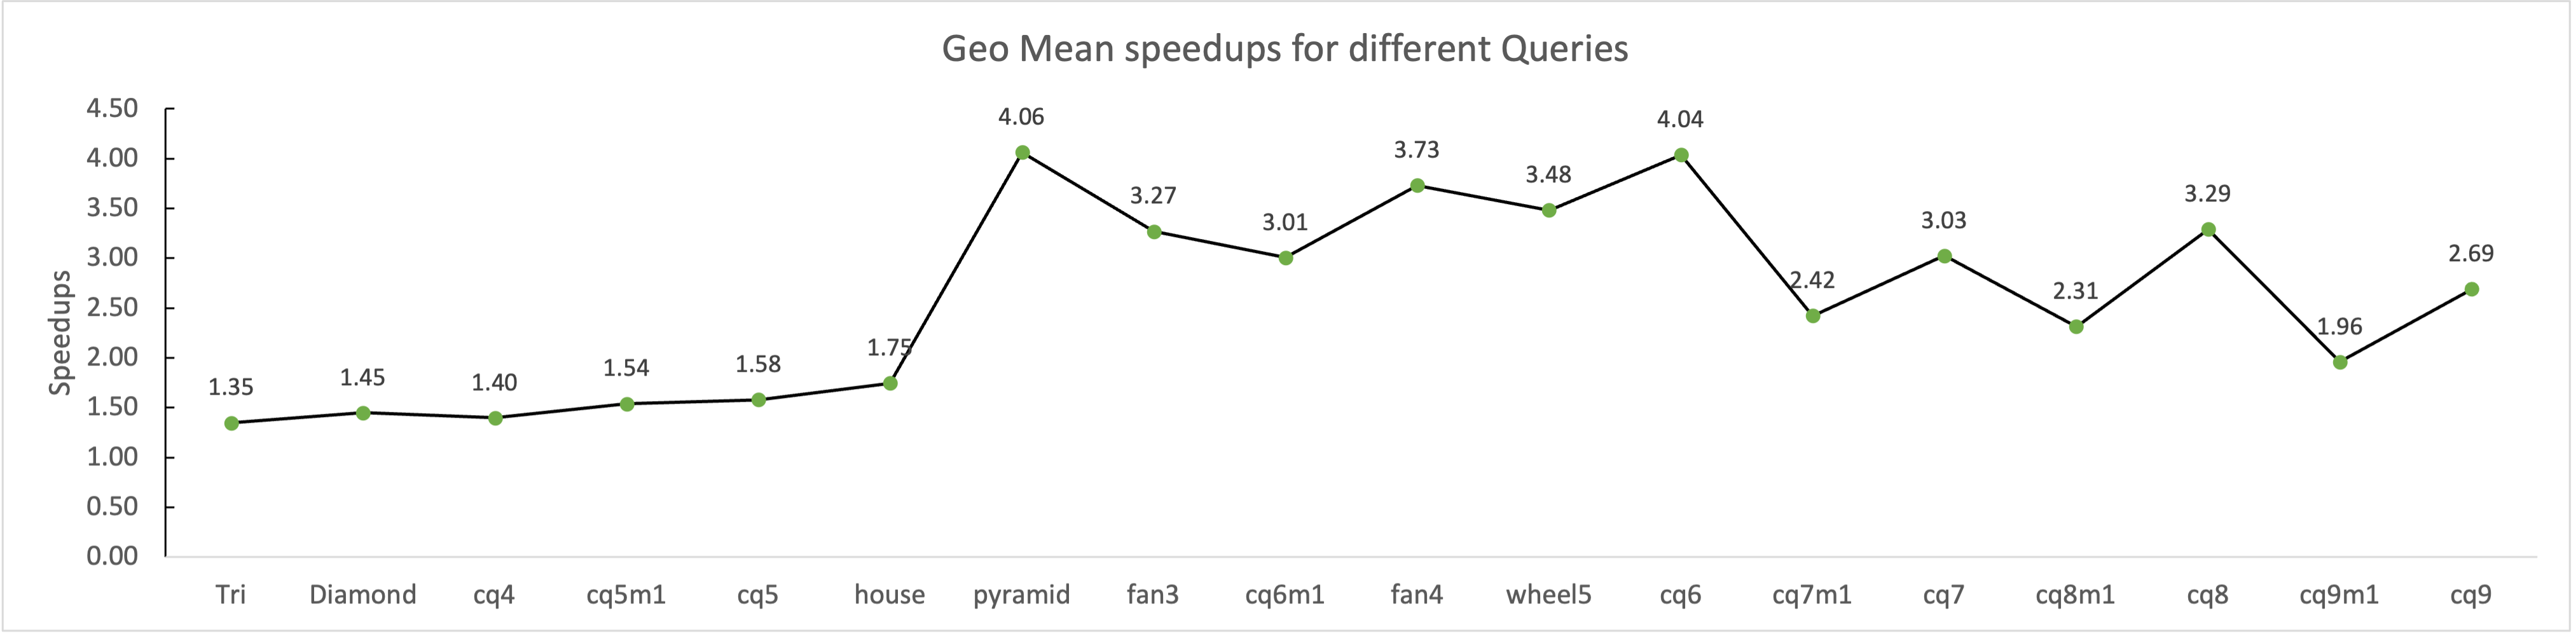
\includegraphics[width=\textwidth]{fig/Results/query-speedups.png}
    \caption{Geo Mean speedups across all data graphs}
    \label{fig:query-speedups}
\end{figure}

\chapter{Conclusions and Future Work}\label{chap:conclusions}

In this thesis, a comprehensive review of subgraph enumeration algorithms using state space search techniques was conducted.
Insights from traditional sequential algorithms and understanding of GPU architecture were used to uncover several enhancements on the state-of-the-art subgraph enumeration application, PARSEC \cite{PARSEC_VD}.
To reduce the number of intersections, the problem of detecting optimal reuse mappings was posed as an optimization problem and a closed form solution was found.
The search space of the search tree was shrunk by using a two-phase hybrid symmetry breaking strategy which uses heuristics to dynamically decide the symmetry breaking direction.
Further, an in-depth analysis of PARSEC \cite{PARSEC_VD} was performed to reveal the underlying load imbalance due to the parallelization scheme and static work division.
The load balance was improved by using a hybrid parallelization scheme that switches after a cutoff.
These different techniques help achieve modest geometric mean speedups of up to $4\times$ across different data graphs and up to $3.7\times$ across all queries. A maximum speedup of $14.6\times$ was attained.
These efforts also help develop numerous computational insights to unlock scope for further improvements.

For future work, the load balance can be improved by using dynamic strategies like work sharing between blocks.
The biggest drawback of this implementation is that it is only applicable for queries with a central node.
Different algorithms need to be developed for supporting more queries.
One idea might be to convert edges in query graphs to vertices to support queries with a central edge.
Another could be to add dummy edges to queries to create an artificial central node.

Another drawback of this implementation is that the memory requirement is in the order of the square of undirected max degree. This restricts the implementation to be truly scalable for large dense graphs. However, real world graphs generally have few vertices with very high degree, these can be dealt with using CPU where the memory is not too restrictive.
Orientation-based techniques were attempted which store induced subgraphs of the oriented graph and find rest of the candidates using binary search.
However, these implementations do not perform well with increasing query size and have even worse load balance.

After addressing the load balance problems, this implementation can be scaled to multiple GPUs by using the CPU unified memory to store the data graph and process even bigger data graphs and larger queries in reasonable time.
Graph partition packages like METIS \cite{metis} can be utilized to scale to multiple CPUs.
This will produce a truly scalable high performing subgraph enumerator unlocking new applications on much larger data graphs.



%%%%%%%%%%%%%%%%%%%%%%%%%%%%%%%%%%%%%%%%%%%%%%%%%%%%%%%%%%%%%%%%%%%%%%%%%%%%%%%
% APPENDIX
%
\appendix
\include{tex/apx}

\backmatter

%%%%%%%%%%%%%%%%%%%%%%%%%%%%%%%%%%%%%%%%%%%%%%%%%%%%%%%%%%%%%%%%%%%%%%%%%%%%%%%
% BIBLIOGRAPHY
%
\bibliographystyle{IEEE_ECE}
% Put references in BibTeX format in thesisrefs.bib.
\bibliography{thesisrefs}


%%%%%%%%%%%%%%%%%%%%%%%%%%%%%%%%%%%%%%%%%%%%%%%%%%%%%%%%%%%%%%%%%%%%%%%%%%%%%%%
% AUTHOR'S BIOGRAPHY
% As of 10/03/2011, Author's Biography or Vita no longer accepted by Grad College

\end{document}
\endinput
